\documentclass[11pt,a4paper,twoside,openany]{book}
\usepackage{import}
\subimport{../}{style}
\subimport{../}{macros}
\subimport{../}{glossary}
\graphicspath{{../img/}}
\makeglossaries
\makeindex
%TODO:
% - crossref chapters & co
% - \n\n -> \n
% - soorten quotes
% - i.e. -> i.e.,
% - e.g. -> e.g.,
% - files, urls, \ldots -> \texttt
%

\begin{document}

\pagestyle{empty}

 \begin{center}

\includegraphics*[width=8truecm]{logo_vsc}

\vspace*{1.5\baselineskip}

\Huge \strong{HPC Tutorial} \\
\LARGE Version 20180831.02

\ifwindows
\LARGE For Windows Users
\fi
\ifmac
\LARGE For macOS Users
\fi
\iflinux
\LARGE For Linux Users
\fi

\vspace*{.75\baselineskip}
\ifantwerpen
\includegraphics*[width=7truecm]{logo_ua}
\fi

\vspace*{0.75\baselineskip}


\normalsize\strong{Author:}

Geert Borstlap (UAntwerpen)

\vspace*{.5\baselineskip}

\strong{Co-authors:}

Kenneth Hoste, Toon Willems, Jens Timmerman (UGent)

Geert-Jan Bex (UHasselt and KU~Leuven)

Mag Selwa (KU~Leuven)

Stefan Becuwe, Franky Backeljauw, Bert Tijskens, Kurt Lust (UAntwerpen)

Bal\'azs Hajgat\'o (VUB)

\vspace*{.5\baselineskip}

Acknowledgement: VSCentrum.be

\vspace*{\baselineskip}

\begin{tabular}{ >{\centering\arraybackslash}m{0.25\textwidth}  >{\centering\arraybackslash}m{0.05\textwidth}  >{\centering\arraybackslash}m{0.20\textwidth}  >{\centering\arraybackslash}m{0.2\textwidth}} \\
\includegraphics*[width=0.2\textwidth, height=0.7in, keepaspectratio=true]{logo_auha} & \multicolumn{2}{ >{\centering\arraybackslash}m{.2\textwidth} }{\includegraphics*[width=0.2\textwidth, height=0.7in,, keepaspectratio=true]{logo_akuleuven}} & \includegraphics*[width=0.2\textwidth, height=0.7in,, keepaspectratio=true]{logo_auhl} \\
\multicolumn{2}{ >{\centering\arraybackslash}m{.32\textwidth} }{\includegraphics*[width=0.3\textwidth, height=0.7in, keepaspectratio=true]{logo_augent}} & \multicolumn{2}{ >{\centering\arraybackslash}m{.38\textwidth} }{\includegraphics*[width=0.3\textwidth, height=0.7in, keepaspectratio=false]{logo_uab}} \\
\end{tabular}
\end{center}


\cleardoublepage
\pagestyle{plain}
\strong{Audience:}

This HPC Tutorial is designed for \strong{researchers} at the
\strong{\university} and affiliated institutes who are in need of
computational power (computer resources) and wish to explore and use the High
Performance Computing (HPC) core facilities of the Flemish Supercomputing Centre (VSC)
to execute their computationally intensive tasks.


The audience may be completely unaware of the \hpc concepts but must have some
basic understanding of computers and computer programming.


\strong{\underbar{Contents:}}

This \strong{Beginners Part} of this tutorial gives answers to the typical
questions that a new \hpc user has. The aim is to learn how to make use of the
HPC.

\begin{tabular}{|p{\dimexpr 0.44\textwidth-2\tabcolsep}|>{\centering\arraybackslash}p{\dimexpr 0.12\textwidth-2\tabcolsep}|p{\dimexpr 0.44\textwidth-2\tabcolsep}|} \hline
\multicolumn{3}{|c|}{\strong{Beginners Part}} \\ \hline
\strong{Questions}                                                      & \strong{chapter} & \strong{title} \\ \hline
What is a \hpc exactly?\newline Can it solve my computational needs?    & \strong{\ref{ch:introduction-to-hpc}} & \nameref{ch:introduction-to-hpc} \\ \hline
How to get an account?                                                  & \strong{\ref{ch:getting-a-hpc-account}} & \nameref{ch:getting-a-hpc-account} \\ \hline
How do I connect to the \hpc and transfer my files and programs?        & \strong{\ref{ch:preparing-the-environment}} & \nameref{ch:preparing-the-environment} \\ \hline
How to start background jobs?                                           & \strong{\ref{ch:running-batch-jobs}} & \nameref{ch:running-batch-jobs} \\ \hline
How to start jobs with user interaction?                                & \strong{\ref{ch:running-interactive-jobs}} & \nameref{ch:running-interactive-jobs} \\ \hline
Where do the input and output go? Where to collect my results?          & \strong{\ref{ch:running-jobs-with-input-output-data}} & \nameref{ch:running-jobs-with-input-output-data} \\ \hline
Can I speed up my program by exploring parallel programming techniques? & \strong{\ref{ch:multi-core-jobs-parallel-computing}} & \nameref{ch:multi-core-jobs-parallel-computing} \\ \hline
Can I start many jobs at once?                                          & \strong{\ref{ch:multi-job-submission}} & \nameref{ch:multi-job-submission} \\ \hline
What are the rules and priorities of jobs?                              & \strong{\ref{ch:hpc-policies}} & \nameref{ch:hpc-policies} \\ \hline
\end{tabular}

The \strong{Advanced Part} focuses on in-depth issues. The aim is to assist the
end-users in running their own software on the \hpc.

\begin{tabular}{|p{\dimexpr 0.44\textwidth-2\tabcolsep}|>{\centering\arraybackslash}p{\dimexpr 0.12\textwidth-2\tabcolsep}|p{\dimexpr 0.44\textwidth-2\tabcolsep}|} \hline
\multicolumn{3}{|c|}{\strong{Advanced Part}} \\ \hline
\strong{Questions}                           & \strong{chapter} & \strong{title} \\ \hline
Can I compile my software on the \hpc?       & \strong{\ref{ch:compiling-and-testing-your-software-on-the-hpc}}      & \nameref{ch:compiling-and-testing-your-software-on-the-hpc} \\ \hline
What are the optimal Job Specifications?     & \strong{\ref{ch:fine-tuning-job-specifications}}      & \nameref{ch:fine-tuning-job-specifications} \\ \hline
%How do I check my programs at runtime?       & \strong{\ref{ch:monitoring-cluster-utilization}}      & \nameref{ch:monitoring-cluster-utilization} \\ \hline
%Can I stop my program and continue later on? & \strong{\ref{ch:checkpointing}}      & Checkpointing \\ \hline
Do you have more examples for me?            & \strong{\ref{ch:program-examples}}      & \nameref{ch:program-examples} \\ \hline
Any more advice?                             & \strong{\ref{ch:best-practices}}      & \nameref{ch:best-practices} \\ \hline
\end{tabular}

The \strong{Annexes} contains some useful reference guides.

\begin{tabular}{|l|c|} \hline
\multicolumn{2}{|c|}{\strong{Annex}} \\ \hline
\strong{Title}             & \strong{chapter} \\ \hline
\nameref{ch:quick-reference-guide} & \strong{\ref{ch:quick-reference-guide}} \\ \hline
\nameref{ch:torque-options}& \strong{\ref{ch:torque-options}} \\ \hline
\nameref{ch:useful-linux-commands}& \strong{\ref{ch:useful-linux-commands}} \\ \hline
\end{tabular}


\strong{\underbar{Notification:}}

In this tutorial specific commands are separated from the accompanying text:

\begin{prompt}
%\shellcmd{commands}%
\end{prompt}

These should be entered by the reader at a command line in a Terminal on the \hpcInfra. They appear in all exercises preceded by a \$ and printed in \textbf{bold}. You'll find those actions in a grey frame.

\keys{Button} are menus, buttons or drop down boxes to be pressed or selected.

``Directory'' is the notation for directories (called ``folders'' in
Windows terminology) or specific files. (e.g., ``\homedir'')

``Text'' Is the notation for text to be entered.

\begin{tip}
A ``Tip'' paragraph is used for remarks or tips.
\end{tip}

\strong{\underbar{More support:}}

Before starting the course, the example programs and configuration files used in this Tutorial must be copied to your home directory, so that you can work with your personal copy. If you have received a new VSC-account, all examples are present in an ``\examplesdir'' directory.

\begin{prompt}
%\shellcmd{cp --r \examplesdir \tilde/}%
%\shellcmd{cd}%
%\shellcmd{ls}%
\end{prompt}

They can also be downloaded from the VSC website at
\url{https://www.vscentrum.be}.
Apart from this \hpc Tutorial, the documentation on the VSC website
will serve as a reference for all the
operations.


\begin{tip}
The users are advised to get self-organised. There are
only limited resources available at the \hpc, which are best effort based.
The \hpc cannot give support for code fixing, the user applications and own
developed software remain solely the responsibility of the end-user.
\end{tip}

More documentation can be found at:

\begin{enumerate}
  \item  VSC documentation: \url{https://www.vscentrum.be/en/user-portal}
  \ifantwerpen
    \item CalcUA Core Facility web pages: \url{https://www.uantwerpen.be/hpc}
  \fi
  \ifbrussel
    \item \hpcname documentation: \url{http://cc.ulb.ac.be/hpc}
  \fi
  \ifgent
    \item \hpcname documentation: \url{http://hpc.ugent.be/userwiki}
  \fi
  \item  External documentation (TORQUE, Moab): \url{http://docs.adaptivecomputing.com}
\end{enumerate}

This tutorial is intended for users who want to connect and work on the HPC of the \strong{\university}.

This tutorial is available in a Windows, Mac or Linux version.

This tutorial is available for UAntwerpen, UGent, KU~Leuven, UHasselt and VUB users.

Request your appropriate version at \hpcinfo.

\strong{\underbar{Contact Information:}}

We welcome your feedback, comments and suggestions for improving the \hpc
Tutorial  (contact: \hpcinfo).

For all technical questions, please contact the \hpc staff:

\inputsite{contact-information}




\glsaddall
\glstoctrue
\renewcommand*{\glsclearpage}{}
\printglossaries

%\cleardoublepage
%\addcontentsline{toc}{chapter}{Index}
\printindex


\tableofcontents

\part{Beginner's Guide}

\pagestyle{vsc}

%Objective:
%
%to learn how to use the \hpc

\chapter{Introduction to HPC}
\label{ch:introduction-to-hpc}

\section{What is HPC?}
\label{sec:what-is-hpc}

``\strong{High Performance Computing}'' (HPC) is computing on a
``\emph{Supercomputer}'', a computer with at the frontline of contemporary
processing capacity -- particularly speed of calculation and available memory.

While the supercomputers in the early days (around 1970) used only a few
processors, in the 1990s machines with thousands of processors began to appear
and, by the end of the 20th century, massively parallel supercomputers with
tens of thousands of ``off-the-shelf'' processors were the norm. A large number
of dedicated processors are placed in close proximity to each other in a
computer cluster.

A \strong{computer cluster} consists of a set of loosely or tightly connected
computers that work together so that in many respects they can be viewed as a
single system.

The components of a cluster are usually connected to each other through fast
local area networks (``LAN'') with each \emph{node} (computer used as a
server) running its own instance of an operating system. Computer clusters
emerged as a result of convergence of a number of computing trends including
the availability of low cost microprocessors, high-speed networks, and software
for high performance distributed computing.

Compute clusters are usually deployed to improve performance and availability
over that of a single computer, while typically being more cost-effective
than single computers of comparable speed or availability.

Supercomputers play an important role in the field of computational science,
and are used for a wide range of computationally intensive tasks in various
fields, including quantum mechanics, weather forecasting, climate research, oil
and gas exploration, molecular modelling (computing the structures and
properties of chemical compounds, biological macromolecules, polymers, and
crystals), and physical simulations (such as simulations of the early moments
of the universe, airplane and spacecraft aerodynamics, the detonation of
nuclear weapons, and nuclear fusion).%
\footnote{Wikipedia: \url{http://en.wikipedia.org/wiki/Supercomputer}}

\section{What is the \hpcInfra?}
\label{sec:what-is-the-hpc}

The \hpc is a collection of computers with
AMD and/or Intel CPUs, running a Linux
operating system, shaped like pizza boxes and stored above and next
to each other in racks, interconnected with copper and fiber cables. Their
number crunching power is (presently) measured in hundreds of billions of
floating point operations (gigaflops) and even in teraflops.

\begin{center}
\includegraphics*[width=1.88in, height=1.26in, keepaspectratio=false]{ch1-cables1}
\includegraphics*[width=1.88in, height=1.26in, keepaspectratio=false]{ch1-cables2}
\includegraphics*[width=1.88in, height=1.26in, keepaspectratio=false]{ch1-cables3}
\end{center}

The \hpcInfra relies on parallel-processing technology to offer \university researchers an
extremely fast solution for all their data processing needs.


\ifantwerpen
The \hpc consists of:
\begin{center}
\begin{tabular}{|p{1.8in}|p{2.1in}|} \hline
\strong{In technical terms}         & \strong{\dots\  in human terms}                    \\ \hline
over 280 nodes and over 11000 cores            & \dots\  or the equivalent of 2750 quad-core PCs    \\ \hline
over 500 Terabyte of online storage     & \dots\  or the equivalent of over 60000 DVDs            \\ \hline
up to 100 Gbit InfiniBand fiber connections & \dots\  or allowing to transfer 3 DVDs per second \\ \hline
\end{tabular}
\end{center}
\fi
%TODO insert specs for other sites

The \hpc currently consists of:

\ifantwerpen
Leibniz:
  \begin{enumerate}
  \item 144 compute nodes with 2 14-core Intel E5-2680v4 CPUs (Broadwell generation, 2.4 GHz) and 128 GB RAM, 120 GB local disk
  \item 8 compute nodes with 2 14-core Intel E5-2680v4 CPUs (Broadwell generation, 2.4 GHz) and 256 GB RAM, 120 GB local disk
  \item 24 ``hopper'' compute nodes (recovered from the former Hopper cluster) with 2 ten core Intel E5-2680v2 CPUs (Ivy Bridge generation, 2.8 GHz), 256 GB memory, 500 GB local disk
  \item 2 GPGPU nodes with 2 14-core Intel E5-2680v4 CPUs (Broadwell generation, 2.4 GHz), 128 GB RAM and two NVIDIA Tesla P100 GPUs with 16 GB HBM2 memory per GPU, 120 GB local disk
  \item 1 vector computing node with 1 12-core Intel Xeon Gold 6126 (Skylake generation, 2.6 GHz), 96 GB RAM and 2 NEC SX-Aurora Vector Engines type 10B (per card 8 cores @1.4 GHz, 48 GB HBM2), 240 GB local disk
  \item 1 Xeon Phi node with 2 14-core Intel E5-2680v4 CPUs (Broadwell generation, 2.4 GHz), 128 GB RAM and Intel Xeon Phi 7220P PCIe card with 16 GB of RAM, 120 GB local disk
  \item 1 visualisation node with 2 14-core Intel E5-2680v4 CPUs (Broadwell generation, 2.4 GHz), 256 GB RAM and with a NVIDIA P5000 GPU, 120 GB local disk
  \end{enumerate}
The nodes are connected using an InfiniBand EDR network except for the ``hopper'' compute nodes that utilize FDR10 InfiniBand. 

Vaughan:
  \begin{enumerate}
  \item 104 compute nodes with 2 32-core AMD Epyc 7452 (2.35 GHz) and 256 GB RAM, 240 GB local disk
  \end{enumerate}
The nodes are connected using an InfiniBand HDR100 network.

\fi
\ifleuven
  \begin{enumerate}
     \item ThinKing (thin node cluster)
      \begin{itemize}
       \item  176 compute nodes with 2 10-core Ivy Bridge processors, 64 GB memory,
              300 GB local disk, QDR-IB network
       \item  32 compute nodes with 2 10-core Ivy Bridge processors, 128 GB memory,
              300 GB local disk, QDR-IB network
       \item  48 compute nodes with 2 12-core Ivy Bridge processors, 64 GB memory,
              300 GB local disk, QDR-IB network
      \end{itemize}
    \item Accelerator partition
      \begin{itemize}
       \item  8 nodes with 2 8-core Sandy Bridge processors, 64 GB memory,
              300 GB local disk, DDR-IB network, 2 K20 NVIDIA GPGPUs
       \item  8 nodes with 2 8-core Sandy Bridge processors, 64 GB memory,
              300 GB local disk, DDR-IB network, 2 Intel Xeon Phis
       \item  4 nodes with 2 6-core Xeon 5650 Westmere processors, 24 GB memory,
              300 GB local disk, DDR-IB network, 2 Tesla M2070 GPGPUs
       \item  5 nodes with 2 10-core Haswell Xeon E5-2650v3 processors, 64 GB memory,
              300 GB local disk, DDR-IB network, 2 Tesla K40 GPGPUs
      \end{itemize}
    \item Visualization partition
      \begin{itemize}
       \item  2 nodes with 2 10-core Haswell Xeon E5-2650v3 processors, 128 GB memory,
              300 GB local disk, DDR-IB network, 2 NVIDIA Quadro K5200 GPUs (visualization nodes)
      \end{itemize}
    \item Cerebro (shared memory SMP section)
      \begin{itemize}
        \item  64 sockets with 10-core Xeon E5-4650 processors, total 14 TB memory,
               SGI-proprietary NUMAlink6 interconnect,
               1 partition has 480 cores and 12 TB RAM and another partition has 160 cores and 2 TB RAM,
               both partitions have 10TB local scratch space
      \end{itemize}
  \end{enumerate}
\fi
\ifbrussel
  a mix of nodes with AMD and Intel CPUs and different interconnects in different sections of the cluster. The cluster also contains a number of nodes with NVIDIA GPGPUs.  For an up to date list of all clusters and their hardware, see\\*
  \url{https://vscdocumentation.readthedocs.io/en/latest/brussels/tier2_hardware.html}.
\fi
\ifgent
  a set of different compute clusters. For an up to date list of all clusters and their hardware, see\\*
  \url{https://vscdocumentation.readthedocs.io/en/latest/gent/tier2_hardware.html}.
\fi
%TODO other sites: keep up to date, or link to vsc website?

\ifantwerpen
All the nodes in the \hpc run under the ``\operatingsystem'' operating
system, which is a clone of ``\operatingsystembase'',
with \emph{cgroups} support.
\fi
\ifleuven
All the nodes in the \hpc run under the ``\operatingsystem'' operating system.
\fi
\ifbrussel
All the nodes in the \hpc run under the ``\operatingsystem'' operating
system, which is a clone of ``\operatingsystembase'',
with \emph{cpuset} support.
\fi
%TODO insert specs for other sites

\ifgent
\strong{Job management} and \strong{job scheduling} are performed by Slurm with a Torque frontend. We advise users to adhere to Torque commands mentioned in this document.
\else
Two tools perform the \strong{job management} and \strong{job scheduling}:
\begin{enumerate}
  %TODO: this gives weird rendering artifacts??
  \item  TORQUE: a resource manager (based on PBS);
  \item  Moab: job scheduler and management tools.
\end{enumerate}
\fi

\ifantwerpen
%\strong{Accounting} is handled by a third tool, i.e., GOLD.
\fi
\ifleuven
\strong{Accounting} is handled by a third tool, i.e., MAM (Moab Accounting
Manager).
\fi
%TODO check whether others use accounting

\ifantwerpen
    For maintenance and monitoring, we use:
    \begin{enumerate}
      \item  Ganglia: monitoring software;
      \item  Icinga and Nagios: alert manager.
    \end{enumerate}
\fi
\ifleuven
    For maintenance and monitoring, we use:
    \begin{enumerate}
      \item  Ganglia: monitoring software;
      \item  HP Insight Cluster Management Utility.
    \end{enumerate}
\fi
\ifbrussel
    For maintenance and monitoring, we use:
    \begin{enumerate}
      \item  Bright Cluster Manager;
      \item  Zabbix: monitoring system.
    \end{enumerate}
\fi
%TODO check tools for other sites


\section{What the HPC infrastucture is \emph{not}}
\label{sec:what-is-the-hpc-not}

The HPC infrastructure is \emph{not} a magic computer that automatically:
\begin{enumerate}
  \item  runs your PC-applications much faster for bigger problems;
  \item  develops your applications;
  \item  solves your bugs;
  \item  does your thinking;
  \item  \dots
  \item  allows you to play games even faster.
\end{enumerate}
The \hpc does not replace your desktop computer.

\section{Is the \hpc a solution for my computational needs?}
\label{sec:is-the-hpc-a-solution-for-my-computational-needs}

\subsection{Batch or interactive mode?}
\label{sec:batch-or-interactive-mode}

Typically, the strength of a supercomputer comes from its ability to run a huge
number of programs (i.e., executables) in parallel without any user interaction
in real time. This is what is called ``running in batch mode''.

It is also possible to run programs at the \hpc, which require user
interaction. (pushing buttons, entering input data, etc.).  Although
technically possible, the use of the \hpc might not always be the best and
smartest option to run those interactive programs.  Each time some user
interaction is needed, the computer will wait for user input. The available
computer resources (CPU, storage, network, etc.) might not be optimally used in
those cases. A more in-depth analysis with the \hpc staff can unveil whether
the \hpc is the desired solution to run interactive programs.
Interactive mode is typically only useful for creating quick visualisations
of your data without having to copy your data to your desktop and back.
%TODO: only visualization nodes should be used interactively

\subsection{What are cores, processors and nodes?}

In this manual, the terms core, processor and node will be frequently used,
so it's useful to understand what they are.

Modern servers, also referred to as \emph{(worker)nodes} in the context of HPC,
include one or more sockets, each housing a multi-\emph{core} \emph{processor} (next to
memory, disk(s), network cards, \ldots). A modern \emph{processor} consists of
multiple CPUs or \emph{cores} that are used to execute \emph{computations}.

\subsection{Parallel or sequential programs?}
\label{sec:parallel-or-sequential-programs}

\subsubsection{Parallel programs}


\strong{Parallel computing} is a form of computation in which many calculations
are carried out simultaneously. They are based on the principle that large
problems can often be divided into smaller ones, which are then solved
concurrently (``in parallel'').

Parallel computers can be roughly classified according to the level at which
the hardware supports parallelism, with multicore computers having multiple
processing elements within a single machine, while clusters use multiple
computers to work on the same task. Parallel computing has become the dominant
computer architecture, mainly in the form of multicore processors.

The two parallel programming paradigms most used in HPC are:

\begin{itemize}
    \item OpenMP for shared memory systems (multithreading): on multiple cores of a single node
    \item MPI for distributed memory systems (multiprocessing): on multiple nodes
\end{itemize}

\strong{Parallel programs} are more difficult to write than sequential ones,
because concurrency introduces several new classes of potential software bugs,
of which race conditions are the most common. Communication and synchronisation
between the different subtasks are typically some of the greatest obstacles to
getting good parallel program performance.

\subsubsection{Sequential programs}

Sequential software does not do calculations in parallel, i.e., it only uses
\emph{one single core of a single workernode}. \strong{It does not become
faster by just throwing more cores at it}: it can only use one core.

It is perfectly possible to also run purely \strong{sequential programs} on the
\hpc.

Running your sequential programs on the most modern and fastest computers in
the \hpc can save you a lot of time.  But it also might be possible to run
multiple instances of your program (e.g., with different input parameters) on
the \hpc, in order to solve one overall problem (e.g., to perform a parameter
sweep). This is another form of running your sequential programs in parallel.

\subsection{What programming languages can I use?}
\label{sec:what-programming-languages-can-i-use}

You can use \emph{any} programming language, \emph{any} software package and
\emph{any} library provided it has a version that runs on Linux, specifically,
on the version of Linux that is installed on the compute nodes,
\operatingsystem.

For the most common \strong{programming languages}, a compiler is available on
\operatingsystem. Supported and common programming languages on the \hpc are
C/C++, FORTRAN, Java, Perl, Python, MATLAB, R, etc.

Supported and commonly used compilers are
%TODO insert compilers for other sites
\ifantwerpen
GCC, clang, J2EE and Intel Cluster Studio.
\fi
\ifleuven
GCC, Intel and PGI.
\fi
\ifbrussel
GCC, clang, J2EE and Intel Cluster Studio.
\fi
\ifgent
GCC and Intel.
\fi

%TODO insert software for other sites

\ifantwerpen
Commonly used software packages are:
\begin{itemize}
\item{in bioinformatics: beagle, Beast, bowtie, MrBayes, SAMtools}
\item{in chemistry: ABINIT, CP2K, Gaussian, Gromacs, LAMMPS, NWChem, Quantum Espresso, Siesta, VASP}
\item{in engineering: COMSOL, OpenFOAM, Telemac}
\item{in mathematics: JAGS, MATLAB, R}
\item{for visuzalization: Gnuplot, ParaView.}
\end{itemize}

Commonly used libraries are Intel MKL, FFTW, HDF5, PETSc and Intel MPI,
OpenMPI.
\fi
\ifleuven
Commonly used software packages are:
\begin{itemize}
\item{in bioinformatics: beagle, Beast, bedtools, bowtie, BWA, Mr. Bayes, TopHat, TRIQS,}
\item{in chemistry: CP2K, Gaussian, GROMACS, Molpro, NAMD, NWChem, Siesta, Turbomole, VASP, VMD,}
\item{in engineering: Abaqus, Ansys, Comsol, OpenFOAM,}
\item{in mathematics: JAGS, MATLAB, R, SAS,}
\item{for visuzalization: Gnuplot, IDL, Paraview, Tecplot, VisIt.}
%\ldots
\end{itemize}


Commonly used libraries are: Intel MKL, FFTW, HDF5, PETSc, Intel MPI,
M(VA)PICH, OpenMPI, Qt, VTK and Mesa.
\fi
\ifbrussel
Commonly used software packages are CP2K, Gaussian, MATLAB, NWChem, R, \ldots

Commonly used Libraries are Intel MKL, FFTW, HDF5, netCDF, PETSc and Intel MPI,
OpenMPI.
\fi

Additional software can be installed ``\emph{on demand}''. Please contact the
\hpc staff to see whether the \hpc can handle your specific requirements.

\subsection{What operating systems can I use?}
\label{sec:what-operating-systems-can-i-use}

All nodes in the \hpc cluster run under \operatingsystem, which is a specific
version of \operatingsystembase. This means that all programs (executables)
should be compiled for \operatingsystem.

Users can connect from any computer in the \university network to the
\hpc, regardless of the Operating System that they are using on their personal
computer.
Users can use any of the common Operating Systems (such as Windows, macOS or
any version of Linux/Unix/BSD) and run and control their programs on the \hpc.

A user does not need to have prior knowledge about Linux; all of the required
knowledge is explained in this tutorial.

\subsection{What does a typical workflow look like?}

A typical workflow looks like:

\begin{enumerate}
    \item Connect to the login nodes with SSH (see \autoref{sec:first-time-connection-to-the-hpc})
    \item Transfer your files to the cluster (see \autoref{sec:filetransfer})
    \item Optional: compile your code and test it (for compiling, see \autoref{ch:compiling-and-testing-your-software-on-the-hpc})
    \item Create a job script and submit your job (see \autoref{ch:running-batch-jobs})
    \item Get some coffee and be patient:
    \begin{enumerate}
        \item Your job gets into the queue
        \item Your job gets executed
        \item Your job finishes
    \end{enumerate}
    \item Study the results generated by your jobs, either on the cluster or after downloading them locally.
\end{enumerate}


\subsection{What is the next step?}
\label{sec:what-is-the-next-step}

When you think that the \hpc is a useful tool to support your computational
needs, we encourage you to acquire a VSC-account (as explained in
\autoref{ch:getting-a-hpc-account}), read
\autoref{ch:connecting}, ``Setting up the environment'', and
explore chapters~\ref{ch:running-interactive-jobs}
to~\ref{ch:fine-tuning-job-specifications} which will help you to transfer and
run your programs on the \hpc cluster.

Do not hesitate to contact the \hpc staff for any help.


\chapter{Getting an HPC Account}
\label{ch:getting-a-hpc-account}

\section{Getting ready to request an account}
\label{sec:getting-ready-to-request-an-account}

All users of \association can request an account on
the \hpc, which is part of the Flemish Supercomputing Center (VSC).

The VSC, abbreviation of Flemish Supercomputer Center, is a virtual
supercomputer center. It is a partnership between the five Flemish
associations: the Association KULeuven,  Ghent University Association, Brussels
University Association, Antwerp University Association and the University
Colleges-Limburg. The VSC is funded by the Flemish Government.

The \hpc clusters use public/private key pairs for user authentication
(rather than passwords). Technically, the private key is stored on your local
computer and always stays there; the public key is stored on the \hpc.
Access to the \hpc is granted to anyone who can prove to have access to the
corresponding private key on his local computer.

\includegraphics*[width=5.75in, height=3.01in, keepaspectratio=false]{ch2-authentication-general}

Since all VSC clusters use Linux as their main operating system, you will
need to get acquainted with using the command-line interface and using the
Terminal.

% IFDEF WINDOWS
\ifwindows
  A typical Windows environment does not come with pre-installed
  software to connect and run command-line executables on a \hpc. Some tools
  needs to be installed on your Windows machine first, before we can start the
  actual work.

  \subsection{Install Putty: A free telnet/SSH client}
  \label{sec:install-putty}

  We recommend to use the PuTTY tools package, which is freely available. You
  do not need to install PuTTY, you can download the putty and PuTTYgen executable
  and directly run it. This can be usefull in situations where you do not have the
  required permissions to install software on the computer you are using.
  Alternatively, an installation package is also available.

  You can download putty from the official address:
  \url{http://www.chiark.greenend.org.uk/\~sgtatham/putty/}

  The PuTTY package consists of several components:

  \begin{enumerate}
    \item  \strong{PuTTY}: the Telnet and SSH client itself
    \item  \strong{PSCP}: an SCP client, i.e., command-line secure file copy
    \item  \strong{PSFTP}: an SFTP client, i.e., general file transfer sessions much like FTP
    \item  \strong{Plink}: a command-line interface to the PuTTY back ends
    \item  \strong{Pageant}: an SSH authentication agent for PuTTY, PSCP and Plink
    \item  \strong{PuTTYgen}: an RSA and DSA key generation utility
    \item  \strong{pterm}: a standalone terminal emulator
  \end{enumerate}

  \subsection{Generating a public/private key pair}
  \label{sec:generate-key-pair}

  Before requesting a VSC account, you need to generate a pair of \emph{ssh}
  keys. We need 2 keys, a public and a private key. You can visualize the public
  key as a lock to which only you have the key (your private key). You can send
  your lock to anyone without any problems, because only you know how to open it,
  as long as you keep your private key secure.
  To generate a public/private key pair, you can use the PuTTYgen key generator.

  Start \strong{\emph{PuTTYgen.exe}} it and follow these steps:

  \begin{enumerate}
    \item  In \keys{Parameters} (at the bottom of the window), choose
      ``SSH-2 RSA'' and set the number of bits in the key to 2048.

    \includegraphics*[width=3.49in, height=3.38in, keepaspectratio=false]{ch2-puttygen-bits}

    \item  Click on \keys{Generate}. To generate the key, you must move
      the mouse cursor over the PuTTYgen window (this generates some random
      data that PuTTYgen uses to generate the key pair). Once the key pair is
      generated, your public key is shown in the field
      \keys{Public key for pasting into OpenSSH authorized\_keys file}.
    \item  Next, it is advised to fill in the \keys{Key comment} field
      to make it easier identifiable afterwards.
    \item  Next, you should specify a passphrase in the \keys{Key passphrase}
      field and retype it in the \keys{Confirm passphrase} field.
      Remember, the passphrase protects the private key against unauthorized
      use, so it is best to choose one that is not too easy to guess but that
      you can still remember.
      Using a passphrase is not required, but we recommend you to use a good
      passphrase unless you are certain that your computers hard disk is
      encrypted with a decent password. (If you are not sure your disk is
      encrypted, it probably isn\'t.

    \includegraphics*[width=3.39in, height=3.28in, keepaspectratio=false]{ch2-puttygen-password}

    \item  Finally, save both the public and private keys in a folder on your
      personal computer (We recommend to create and put them in the folder
      ``C:\textbackslash Users\textbackslash \%USERNAME\%\textbackslash
      AppData\textbackslash Local\textbackslash PuTTY\textbackslash .ssh'')
      with the buttons \keys{Save public key} and \keys{Save private key}.
      We recommend using the name ``\strong{id\_rsa.pub}'' for the public key,
      and ``\strong{id\_rsa.ppk}'' for the private key.
  \end{enumerate}

  If you use another program to generate a key pair, please remember that they
  need to be in the OpenSSH format to access the \hpc clusters.
\fi %WINDOWS

\ifmac
  To open a Terminal window in OS X, open the Finder and choose

  \emph{$>$$>$ Applications $>$ Utilities $>$ Terminal}
\fi

\iflinux
  To open a Terminal window in Linux, open the Finder and choose

  Launch a terminal from your desktop’s application menu and you will see the bash shell.
  There are other shells, but most Linux distributions use bash by default.
\fi

\ifmacORlinux
  Before requesting an account, you need to generate a pair of ssh keys. One
  popular way to do this on OS X is using the OpenSSH client included with OS
  X, which you can then also use to log on to the clusters.

  \subsection{Test OpenSSH}
  \label{sec:test-openssh}

  Secure Shell (ssh) is a cryptographic network protocol for secure data
  communication, remote command-line login, remote command execution, and other
  secure network services between two networked computers. In short, ssh
  provides a secure connection between 2 computers via insecure channels
  (Network, Internet, telephone lines, \ldots).

  ``Secure'' means that:
  \begin{enumerate}
    \item  the User is authenticated to the System; and
    \item  the System is authenticated to the User; and
    \item  all data is encrypted during transfer.
  \end{enumerate}

  OpenSSH is a FREE implementation of the SSH connectivity protocol. OS X comes
  with its own implementation of OpenSSH, so you don't need to install any
  third-party software to use it. Just open a Terminal window and jump in!

  On all popular Linux distributions, the OpenSSH software is readily
  available, and most often installed by default. You can check whether the
  OpenSSH software is installed by opening a terminal and typing:

\begin{prompt}
%\shellcmd{ssh -V}%
OpenSSH_4.3p2, OpenSSL 0.9.8e-fips-rhel5 01 Jul 2008
\end{prompt}

  To access the clusters and transfer your files, you will use the following commands:

  \begin{enumerate}
    \item  ssh-keygen: to generate the ssh keys
    \item  ssh: to open a shell on a remote machine;
    \item  sftp: a secure equivalent of ftp;
    \item  scp: a secure equivalent of the remote copy command rcp.
  \end{enumerate}

  \subsection{Generate a public/private key pair with OpenSSH}
  \label{sec:generate-key-pair-with-openssh}

  A key pair might already be present in the default location inside your home
  directory. Therefore, we first check if a key is available with the ``list
  short'' (``ls'')  command:

\begin{prompt}
%\shellcmd{ls ~/.ssh}%
\end{prompt}


  If a key-pair is already available, you would normally get:
\begin{prompt}
authorized_keys2    id_rsa            id_rsa.pub         known_hosts
\end{prompt}

  Otherwise, the command will show:

\begin{prompt}
ls: .ssh: No such file or directory
\end{prompt}

  You can recognize a public/private key pair when a pair of files has the same
  name except for the extension ``.pub'' added to one of them. In this particular
  case, the private key is ``id\_rsa'' and public key is ``id\_rsa.pub''. You may
  have multiple keys (not necessarily in the directory ``\tilde/.ssh'') if you or
  your operating system requires this.

  You will need to generate a new key pair, when:
  \begin{enumerate}
    \item  you don't have a key pair yet,
    \item  you forgot the passphrase protecting your private key,
    \item  or your private key was compromised.
  \end{enumerate}

  For extra security, the private key itself is encrypted using a ``passphrase'',
  to prevent anyone from using your private key even when they manage to copy
  it. You have to ``unlock'' the private key by typing the passphrase.

\begin{prompt}
%\shellcmd{ssh-keygen}%
Generating public/private rsa key pair.
Enter file in which to save the key (/home/user/.ssh/id_rsa):
Enter passphrase (empty for no passphrase):
Enter same passphrase again:
Your identification has been saved in /home/user/.ssh/id_rsa.
Your public key has been saved in /home/user/.ssh/id_rsa.pub.
\end{prompt}

  This will ask you for a file name to store the private and public key, and a
  passphrase to protect your private key. It needs to be emphasized that you
  really should choose the passphrase wisely! The system will ask you for it
  every time you want to use the private key that is every time you want to
  access the cluster or transfer your files.

  \strong{Without your key pair, you won't be able to apply for a personal VSC account.}
\fi %macORlinux

\section{Applying for the account}
\label{sec:applying-for-the-account}

Open the following webpage from within the \university campus network (or using a VPN
connection) \url{https://account.vscentrum.be/}

You will be taken to a website of BELNET, where you have to select your ``Home Organization''.
For faster logins in the future you can select the 'Remeber selection' checkboxes.

\includegraphics*[width=5.73in, height=4.00in, keepaspectratio=false]{ch2-browser-authenticate}

Select ``\university'' in the dropdown box.

Click $<$Select$>$

You will now be taken to the authentification page of your institute.

\ifantwerpen
\includegraphics*[width=5.73in, height=4.00in, keepaspectratio=false]{ch2-browser-authenticate-institute}

\strong{The site is only accessible from within the \university
domain}, so the page won't load from, e.g., home. However, you can also get
external access to the \university domain using VPN. We refer to the \university ICT infocenter
for more information.

\subsection{Users of the \association}
\label{sec:users-of-association}

All users (researchers, academic staff, etc.) from the higher education
institutions associated with \university can get a VSC account via the \university. There is not
yet an automated form to request your personal VSC account.

Please e-mail the \hpc staff to get an account (see Contacts information).
You will have to provide a public \emph{ssh} key generated as described
above. Please attach your public key (i.e., the file named ``id\_rsa.pub''),
which you will normally find in your .ssh subdirectory within your HOME
Directory. (i.e., /Users/$<$username$>$/.ssh/id\_rsa.pub).


\fi % END IF ANTWERPEN

\ifgent
You will now have to log in with CAS using your UGent account, and then be requested
to share your Mail and Affiliation with KU Leuven (which actually means the VSC accountpage)
Select the 'Remember' checkbox and click 'Yes, continue'
\fi
%TODO: other institute login information explained here?

After you log in using your \university login and password,
you will be asked to upload the file that contains
your public key, i.e., the file ``id\_rsa.pub'' which you have
generated earlier.

\ifwindows
  This file should have been stored in the directory
  ``\emph{/Users/$<$Username$>$/PuTTY/.ssh/}''.
\fi
\ifmacORlinux
  This file has been stored in the directory ``\emph{\tilde/.ssh/}''.
\fi

\ifmac
\begin{tip}
  As ``.ssh'' is an invisible directory, the Finder will
  not show it by default. The easiest way to access the folder, is by pressing
  Apple-Shift--G, which will allow you to enter the name of a directory, which
  you would like to open in Finder. Here, type ``\tilde/.ssh'' and press enter.
\end{tip}
\fi

After you have uploaded your public key you will receive an email with a link to
confirm your email address. After confirming your email address the VSC staff will
review and if applicable approve your account.

\subsection{Welcome e-mail}
\label{sec:welcome-email}

Within one day, you should receive a Welcome e-mail with your VSC account details.

\begin{flattext}
Dear xxxxxxx,
Your VSC-account has been approved by an administrator.
Your vsc-username is vscxxxxx

Your account should be fully active within one hour.
To check or update your account information please visit
https://account.vscentrum.be/

For further info please visit https://vscentrum.be/neutral/documentation

Kind regards,
-- The VSC administrators
\end{flattext}

Now, you can start using the \hpc.

\section{First Time connection to the \hpc}
\label{sec:first-time-connection-to-the-hpc}

\ifwindows

  \subsection{Open a Terminal}
  \label{sec:windows-open-a-terminal}

  You've generated a public/private key pair with PuTTYgen and have an approved
  account on the VSC clusters.  The next step is to setup the connection to (one
  of) the \hpc.

  In the screenshots, we show the setup for user ``\strong{\emph{vsc20167}}''
  to the \hpc cluster via the loginnode
  ``\strong{\emph{\loginnode}}''.

  \begin{enumerate}
    \item  Start the PuTTY executable $<$\strong{\emph{putty.exe}}$>$ in your
      directory ``\strong{\emph{C:\textbackslash Program Files (x86)\textbackslash PuTTY}}'' and the
      configuration screen will pop up. As you will often use the PuTTY tool,
      we recommend adding a shortcut on your desktop.
    \item  Within the category $<$\strong{\emph{Session}}$>$, in the field
      $<$\strong{\emph{Host Name}}$>$, enter the name of the loginnode of the
      \hpc cluster (i.e., ``\strong{\emph{\loginnode}}'')
      you want to connect to.

    \includegraphics*[width=3.59in, height=3.45in, keepaspectratio=false]{ch2-putty-configuration}

    \item  In the category \menu[,]{Connection,Data}, in
      the field \keys{Auto-login username}, put in
      $<$\emph{vsc-account}$>$, which is your VSC username that you have
      received by mail after your request was approved.

  \includegraphics*[width=3.11in, height=2.99in, keepaspectratio=false]{ch2-putty-configuration2}

    \item  In the category \menu[,]{Connection,SSH,Auth}, in the
      field \keys{Private key file for authentication} click on
      \keys{Browse} and select the private key (i.e., ``id\_rsa.ppk'')
      that you generated and saved above.

  \includegraphics*[width=3.25in, height=3.13in, keepaspectratio=false]{ch2-putty-key-setup}

    \item  In the category \menu[,]{Connection,SSH,X11}, click
      the \keys{Enable X11 Forwarding} checkbox.

  \includegraphics*[width=3.54in, height=3.41in, keepaspectratio=false]{ch2-putty-x-forwarding}

    \item  Now go back to $<$Session$>$, and fill in ``\emph{\hpcname}'' in the
      \keys{Saved Sessions} field and press \keys{Save} to
      store the session information.

  \includegraphics*[width=3.30in, height=3.17in, keepaspectratio=false]{ch2-putty-saved-session}

    \item  Now pressing \keys{Open}, will open a terminal window and
      asks for you passphrase.

  \includegraphics*[width=3.94in, height=2.47in, keepaspectratio=false]{ch2-putty-enter-password}

    \item  The first time you make a connection to the loginnode, a Security
      Alert will appear and you will be asked to verify the authenticity of the
      loginnode.
      \ifgent
      Make sure the fingerprint in the Alert matches \strong{2f:0c:f7:76:87:57:f7:5d:2d:7b:d1:a1:e1:86:19:f3}
      \fi
      %TODO: fingerprints for other institution login nodes?

  \includegraphics*[width=3.91in, height=2.42in, keepaspectratio=false]{ch2-putty-verify-authenticity}

    \item  After entering your correct passphrase, you will be connected to the
      login-node of the \hpc.
    \item  To check you can now ``Print the Working Directory'' (pwd) and check
      the name of the computer, where you have logged in (hostname):

  \begin{prompt}
  %\shellcmd{pwd}%
  %\homedir%
  %\shellcmd{hostname --f}%
  %\loginhost%
  \end{prompt}

    \item  For future PuTTY sessions, just select your saved session (i.e.
      ``\emph{\hpcname}'') from the list, \keys{Load} it and press
      \keys{Open}.
  \end{enumerate}

%ENDIF windos
\fi

\ifmacORlinux
\subsection{Connect}
\label{sec:connect}

The \hpc is only accessible from within the \university campus network, but you can
get external access (e.g., from home) by using a VPN connection.

To make a connection to the \hpc cluster, the ssh command is used:

\begin{prompt}
%\shellcmd{ssh $<$vsc-account$>$@\loginnode}%
\end{prompt}

Here,

\begin{enumerate}
  \item  \emph{$<$vsc-account$>$} is your VSC username that you have received
    by mail after your request was approved (e.g., \userid),
  \item  \emph{``\loginnode''} is the name of the login
    node of the \hpc cluster you want to connect to.
\end{enumerate}

The first time you make a connection to the login node, you will be asked to
verify the authenticity of the login node, e.g.,

\begin{prompt}
%\shellcmd{ssh \userid{}@\loginnode{}}%
The authenticity of host ``%\loginnode% (<IP-adress>)'' can't be established.
RSA key fingerprint is b7:66:42:23:5c:d9:43:e8:b8:48:6f:2c:70:de:02:eb.
Are you sure you want to continue connecting (yes/no)? %\strong{\emph{yes}}%
\end{prompt}

Here, user \userid wants to make a connection to the ``\hpcname'' cluster at
\university via the login node ``\loginnode''.

\strong{Congratulations, you're on the \hpc Super-Computer now!}
Okay, I am on the supercomputer, but where am I?

So, print the current working directory:
\begin{prompt}
%\shellcmd{pwd}%
%\homedir%
\end{prompt}
\fi


Your new private home-directory is ``\homedir''.
Here you can create your own sub-directory structure, copy and prepare your
applications, compile and test them and submit your jobs on the \hpc.

\begin{prompt}
%\shellcmd{cd \tutorialdir}%
%\shellcmd{ls}%
intro-HPC/
intro-Linux/
intro-python/
intro-vi/
\end{prompt}

%TODO: make sure this data is here
This directory currently contains all training material for the use of:

\begin{enumerate}
\item  The \strong{\emph{Introduction to the \hpc}}.
\item  The \strong{\emph{Introduction to Linux}}.
\item  The \strong{\emph{Python}} programming language.
\item  The \strong{\emph{VI}} editor.
\end{enumerate}

More relevant training material to work with the \hpc can always be added
later in this directory.

You can now explore the content of this directory with the ``ls --l''
(\strong{l}ist\strong{s} \strong{l}ong) and the ``cd'' (\strong{c}hange
\strong{d}irectory) commands:

As we are interested in the use of the \strong{\emph{HPC}}, move further to
\strong{\emph{intro-HPC}} and explore the contents up to 2 levels deep:

\begin{prompt}
%\shellcmd{cd intro-HPC}%
%\shellcmd{tree -L 2}%
.
`-- examples
    %\textbar%-- Compiling-and-testing-your-software-on-the-HPC
    %\textbar%-- Fine-tuning-Job-Specifications
    %\textbar%-- Multi-core-jobs-Parallel-Computing
    %\textbar%-- Multi-job-submission
    %\textbar%-- Program-examples
    %\textbar%-- Running-batch-jobs
    %\textbar%-- Running-jobs-with-input
    %\textbar%-- Running-jobs-with-input-output-data
    %\textbar%-- example.pbs
    `-- example.sh
9 directories, 5 files
\end{prompt}

This directory contains:

\begin{enumerate}
  \item This \strong{\emph{HPC Tutorial}} (in either a Mac, Linux or Windows version).
  \item The according \strong{\emph{HPC slides}} (used during training sessions).
  \item A \strong{\emph{docs}} sub-directory, containing interesting \hpc related documents.
  \item An \strong{\emph{examples}} sub-directory, containing all the
    examples that you need in this Tutorial, as well as examples that might be
    useful for your specific applications.
\end{enumerate}

\begin{prompt}
%\shellcmd{cd examples}%
\end{prompt}

\begin{tip}
Typing ``\strong{\emph{cd ex$<$TAB$>$}}'' will generate the
``\strong{\emph{cd examples}}'' command. \strong{Command-line completion
}(also tab completion) is a common feature of the bash command line
interpreter, in which the program automatically fills in partially typed
commands.
\end{tip}

\begin{tip}
For more exhaustive tutorials about Linux usage,
please refer to the following sites:

\begin{enumerate}
  \item \url{http://www.linux.org/lessons/}
  \item \url{http://linux.about.com/od/nwb\_guide/a/gdenwb06.htm}
\end{enumerate}
\end{tip}

The first action is to copy the contents of the \hpc examples directory
to your home directory, so that you have your own personal copy and that
you can start using the examples. The ``-r'' option of the copy command
will also copy the contents of the sub-directories ``\emph{recursively}''.

\begin{prompt}
%\shellcmd{cp --r \examplesdir \tilde/}%
\end{prompt}

Go to your home directory, check your own private examples directory, \dots\  and start working.

%\shellcmd{cd}%
%\shellcmd{ls -l}%

\section{Computation Workflow on the \hpc}
\label{sec:compuation-workflow-on-the-hpc}

A typical Computation workflow will be:

\begin{enumerate}
  \item  Connect to the \hpc
  \item  Transfer your files to the \hpc
  \item  Compile your code and test it
  \item  Create a job script
  \item  Submit your job
  \item  Wait while
  \begin{enumerate}
    \item  your job gets into the queue
    \item  your job gets executed
    \item  your job finishes
  \end{enumerate}
  \item  Move your results
\end{enumerate}

We'll take you through the different tasks one by one in the following
chapters.


% Can't use \hpc in a chapter title
\chapter{Connecting to the HPC infrastructure}
\label{ch:connecting}

Before you can really start using the \hpc clusters, there are several things you need to do or know:

\begin{enumerate}
\item  You need to \textbf{log on to the cluster} using an SSH client to one of the login nodes. This will give you command-line access. The software you'll need to use on your client system depends on its operating system.
\item  Before you can do some work, you'll have to \textbf{transfer the files} that you need from your desktop computer to the cluster. At the end of a job, you might want to transfer some files back.
\item  Optionally, if you wish to use programs with a \textbf{graphical user interface}, you will need an X-server on your client system and log in to the login nodes with X-forwarding enabled.
\item  Often several versions of \textbf{software packages and libraries} are installed, so you need to select the ones you need. To manage different versions efficiently, the VSC clusters use so-called \textbf{modules}, so you will need to select and load the modules that you need.
\end{enumerate}

\section{First Time connection to the HPC infrastucture}
\label{sec:first-time-connection-to-the-hpc}

If you have any issues connecting to the \hpc after you've followed these steps,
see \autoref{sec:connecting-issues} to troubleshoot.

\ifantwerpen
 The \hpc is only accessible from within the \university network, but you can
 get external access (e.g., from home) by using a VPN connection.
\fi

\ifwindows

  \subsection{Open a Terminal}
  \label{sec:windows-open-a-terminal}

  You've generated a public/private key pair with PuTTYgen and have an approved
  account on the VSC clusters.  The next step is to setup the connection to (one
  of) the \hpc.

   In the screenshots, we show the setup for user
\ifantwerpen
``\strong{\emph{vsc20167}}''
\fi
\ifbrussel
``\strong{\emph{vsc20167}}''
\fi
\ifgent
``\strong{\emph{vsc20167}}''
\fi
\ifleuven
``\strong{\emph{vsc30468}}''
\fi
  to the \hpc cluster via the login node
  ``\strong{\emph{\loginnode}}''.

  \begin{enumerate}
    \item  Start the PuTTY executable \lstinline|putty.exe| in your
      directory \lstinline|C:\Program Files (x86)\PuTTY| and the
      configuration screen will pop up. As you will often use the PuTTY tool,
      we recommend adding a shortcut on your desktop.
    \item  Within the category <{}\strong{\emph{Session}}>{}, in the field
      <{}\strong{\emph{Host Name}}>{}, enter the name of the login node of the
      \hpc cluster (i.e., ``\strong{\emph{\loginnode}}'')
      you want to connect to.

\ifantwerpen
      \begin{center}
      \includegraphics*[width=3.59in, height=3.45in, keepaspectratio=false]{ch2-putty-configuration}
      \end{center}
\fi
\ifleuven
      \begin{center}
      \includegraphics*[width=3.59in, height=3.45in, keepaspectratio=false]{ch2-putty-configuration-leuven}
      \end{center}
\fi
\ifbrussel
      \begin{center}
      \includegraphics*[width=3.59in, height=3.45in, keepaspectratio=false]{ch2-putty-configuration}
      \end{center}
\fi
\ifgent
      \begin{center}
      \includegraphics*[width=3.59in, height=3.45in, keepaspectratio=false]{ch2-putty-configuration}
      \end{center}
\fi

    \item  In the category \menu[,]{Connection,Data}, in
      the field \keys{Auto-login username}, put in
      <{}\emph{\userid}>{}, which is your VSC username that you have
      received by e-mail after your request was approved.

\ifantwerpen
      \begin{center}
      \includegraphics*[width=3.11in, height=2.99in, keepaspectratio=false]{ch2-putty-configuration2}
      \end{center}
\fi
\ifleuven
      \begin{center}
      \includegraphics*[width=3.11in, height=2.99in, keepaspectratio=false]{ch2-putty-configuration2-leuven}
      \end{center}
\fi
\ifbrussel
      \begin{center}
      \includegraphics*[width=3.11in, height=2.99in, keepaspectratio=false]{ch2-putty-configuration2}
      \end{center}
\fi
\ifgent
      \begin{center}
      \includegraphics*[width=3.11in, height=2.99in, keepaspectratio=false]{ch2-putty-configuration2}
      \end{center}
\fi

    \item  In the category \menu[,]{Connection,SSH,Auth}, in the
      field \keys{Private key file for authentication} click on
      \keys{Browse} and select the private key (i.e., ``id\_rsa.ppk'')
      that you generated and saved above.

      \begin{center}
      \includegraphics*[width=3.25in, height=3.13in, keepaspectratio=false]{ch2-putty-key-setup}
      \end{center}

    \item  In the category \menu[,]{Connection,SSH,X11}, click
      the \keys{Enable X11 Forwarding} checkbox.

      \begin{center}
      \includegraphics*[width=3.54in, height=3.41in, keepaspectratio=false]{ch2-putty-x-forwarding}
      \end{center}

    \item  Now go back to <{}Session>{}, and fill in ``\emph{\hpcname}'' in the
      \keys{Saved Sessions} field and press \keys{Save} to
      store the session information.

\ifantwerpen
      \begin{center}
      \includegraphics*[width=3.30in, height=3.17in, keepaspectratio=false]{ch2-putty-saved-session}
      \end{center}
\fi
\ifleuven
      \begin{center}
      \includegraphics*[width=3.30in, height=3.17in, keepaspectratio=false]{ch2-putty-saved-session-leuven}
      \end{center}
\fi
\ifbrussel
      \begin{center}
      \includegraphics*[width=3.30in, height=3.17in, keepaspectratio=false]{ch2-putty-saved-session}
      \end{center}
\fi
\ifgent
      \begin{center}
      \includegraphics*[width=3.30in, height=3.17in, keepaspectratio=false]{ch2-putty-saved-session}
      \end{center}
\fi


    \item  Now pressing \keys{Open}, will open a terminal window and
      asks for you passphrase.

\ifantwerpen
      \begin{center}
      \includegraphics*[width=3.94in, height=2.47in, keepaspectratio=false]{ch2-putty-enter-password}
      \end{center}
\fi
\ifleuven
      \begin{center}
      \includegraphics*[width=3.94in, height=2.47in, keepaspectratio=false]{ch2-putty-enter-password-leuven}
      \end{center}
\fi
\ifbrussel
      \begin{center}
      \includegraphics*[width=3.94in, height=2.47in, keepaspectratio=false]{ch2-putty-enter-password}
      \end{center}
\fi
\ifgent
      \begin{center}
      \includegraphics*[width=3.94in, height=2.47in, keepaspectratio=false]{ch2-putty-enter-password}
      \end{center}
\fi

    \item If this is your first time connecting, you will be asked to verify the authenticity of
        the login node. Please see section~\ref{sec:warning-message-new-host} on how to do this.

    \item  After entering your correct passphrase, you will be connected to the
      login-node of the \hpc.
    \item  To check you can now ``Print the Working Directory'' (pwd) and check
      the name of the computer, where you have logged in (hostname):

\begin{prompt}
%\shellcmd{pwd}%
%\homedir{}%
%\shellcmd{hostname --f}%
%\loginhost{}%
\end{prompt}

    \item  For future PuTTY sessions, just select your saved session (i.e.
      ``\emph{\hpcname}'') from the list, \keys{Load} it and press
      \keys{Open}.
  \end{enumerate}

%ENDIF windows
\fi

\ifmacORlinux

  \subsection{Connect}
  \label{sec:connect}


  Open up a terminal and enter the following command to connect to the \hpc.
  \ifmac
  You can open a terminal by navigation to Applications and then Utilities in the finder and open Terminal.app, or enter Terminal in Spotlight Search.
  \fi

\begin{prompt}
%\shellcmd{ssh \userid{}@\loginnode{}}%
\end{prompt}

  Here, user \userid wants to make a connection to the ``\hpcname'' cluster at
  \university via the login node ``\loginnode'', so replace \userid with your own
  vsc id in the above command.

  The first time you make a connection to the login node, you will be asked to
  verify the authenticity of the login node. Please check section~\ref{sec:warning-message-new-host}
  on how to do this.

A possible error message you can get if you previously saved your private key
somewhere else than the default location (\lstinline|$HOME/.ssh/id_rsa|):

\begin{prompt}
%\shellcmd{Permission denied (publickey,gssapi-keyex,gssapi-with-mic).}%
\end{prompt}

In this case, use the \lstinline|-i| option for the \lstinline|ssh| command to specify the location
of your private key. For example:

\begin{prompt}
%\shellcmd{ssh -i /home/example/my\_keys/id\_rsa \userid{}@\loginnode{}}%
\end{prompt}

% ENDIF \ifmacORlinux
\fi

\strong{Congratulations, you're on the \hpc infrastructure now!}
To find out where you have landed you can print the current working directory:

\begin{prompt}
%\shellcmd{pwd}%
%\homedir{}%
\end{prompt}


% TODO The preferred location for storing files, certainly the tutorial-files, should be VSC_DATA at Gent.
Your new private home directory is ``\homedir''.
Here you can create your own subdirectory structure, copy and prepare your
applications, compile and test them and submit your jobs on the \hpc.

\begin{prompt}
%\shellcmd{cd \tutorialdir{}}%
%\shellcmd{ls }%
Intro-HPC/
\end{prompt}

This directory currently contains all training material for the \strong{\emph{Introduction to the \hpc}}.
More relevant training material to work with the \hpc can always be added
later in this directory.

You can now explore the content of this directory with the ``ls --l''
(\strong{l}ist\strong{s} \strong{l}ong) and the ``cd'' (\strong{c}hange
\strong{d}irectory) commands:

As we are interested in the use of the \strong{\emph{HPC}}, move further to
\strong{\emph{Intro-HPC}} and explore the contents up to 2 levels deep:

\begin{prompt}
%\shellcmd{cd Intro-HPC}%
%\shellcmd{tree -L 2}%
.
`-- examples
    |-- Compiling-and-testing-your-software-on-the-HPC
    |-- Fine-tuning-Job-Specifications
    |-- Multi-core-jobs-Parallel-Computing
    |-- Multi-job-submission
    |-- Program-examples
    |-- Running-batch-jobs
    |-- Running-jobs-with-input
    |-- Running-jobs-with-input-output-data
    |-- example.pbs
    `-- example.sh
9 directories, 5 files
\end{prompt}

This directory contains:

\begin{enumerate}
  \item This \strong{\emph{HPC Tutorial}} (in either a Mac, Linux or Windows version).
  %TODO: these are not here yet? \item The according \strong{\emph{HPC slides}} (used during training sessions).
  %TODO: this is not here yet? \item A \strong{\emph{docs}} subdirectory, containing interesting \hpc related documents.
  \item An \strong{\emph{examples}} subdirectory, containing all the
    examples that you need in this Tutorial, as well as examples that might be
    useful for your specific applications.
\end{enumerate}

\begin{prompt}
%\shellcmd{cd examples}%
\end{prompt}

\begin{tip}
Typing \lstinline|cd ex| followed by \keys{\tab} (the Tab-key) will generate the
\lstinline|cd examples| command. \strong{Command-line completion
}(also tab completion) is a common feature of the bash command line
interpreter, in which the program automatically fills in partially typed
commands.
\end{tip}

\begin{tip}
For more exhaustive tutorials about Linux usage, see Appendix \ref{ch:useful-linux-commands}
\end{tip}

The first action is to copy the contents of the \hpc examples directory
to your home directory, so that you have your own personal copy and that
you can start using the examples. The ``-r'' option of the copy command
will also copy the contents of the sub-directories ``\emph{recursively}''.

\begin{prompt}
%\shellcmd{cp --r \examplesdir{} \tilde{}/}%
\end{prompt}

\ifgent
You will now make a doc directory in your home dir and copy the latest version of this document to this directory. We will use this later in this tutorial.

\begin{prompt}
%\shellcmd{mkdir \tilde{}/docs}%
%\shellcmd{cp --r \tutorialdir{}/\jobname{} \tilde{}/}%
\end{prompt}

Go to your home directory, check your own private examples directory, \dots\
and start working.

\begin{prompt}
%\shellcmd{cd}%
%\shellcmd{ls -l}%
\end{prompt}

Upon connecting you will see a login message containing your last login
time stamp and a basic overview of the current cluster utilisation.

\begin{prompt}
Last login: Mon Sep  3 14:00:00 2018 from helios.ugent.be
STEVIN HPC-UGent infrastructure status on Mon, 03 Sep 2018 14:30:00

   cluster - full - free -  part - total - running - queued
             nodes  nodes   free   nodes    jobs      jobs
-------------------------------------------------------------------
  delcatty     72      0     52     127      N/A       N/A
    golett    168      2     16     200      N/A       N/A
    phanpy     15      0      1      16      N/A       N/A
    swalot      0      0      0     128      N/A       N/A
    skitty     69      2      0      73      N/A       N/A
   victini     83      1      3      96      N/A       N/A

For a full view of the current loads and queues see:
 http://hpc.ugent.be/clusterstate/
Updates on maintenance and unscheduled downtime can be found on
 https://www.vscentrum.be/en/user-portal/system-status

\end{prompt}
\fi %ENDIF \ifgent
%
\ifbrussel
Upon connecting you will see a login message containing your last login
time stamp, some useful environment variable definitions and the message of the
day (MOTD).

\begin{prompt}
Last login: Thu Nov  6 16:05:21 2014 from example.vub.ac.be

Initialising your working environment...
System variables to use in your scripts/programs:
  Temporary directory:   \$TMPDIR as /tmp/vsc40485
  Temporary work directory:    \$WORKDIR as /work/vsc40485
  Home directory:              \$HOME as /user/home/gent/vsc404/vsc40485
Message of the day:

  --------------------------------------------------------------------
  Welcome to the Hydra cluster.

  The old work directory access has been closed.


  The Hydra Team
  --------------------------------------------------------------------
       \   ,__,
        \  (oo)____
           (__)    )\
              ||--||

\end{prompt}
\fi %ENDIF \ifbrussel

\ifleuven
Upon connecting you will see a login message containing your last login
time stamp and some useful links.

\begin{prompt}
Last login: Mon Jan 12 18:52:20 2015 from example.kuleuven.be
**********************************************
*                                            *
* Please check the following site for        *
* status messages concerning KU Leuven       *
* services (incl. HPC):                      *
*                                            *
*   http://status.kuleuven.be/               *
*                                            *
* For VSC user documentation:                *
*                                            *
*  https://www.vscentrum.be/en/user-portal   *
*                                            *
*                                            *
**********************************************
\end{prompt}
\fi  % ENDIF \ifleuven

\ifantwerpen
Upon connection, you will get a welcome message containing your last login
timestamp and some pointers to information about the system. On Hopper, the system
will also show your disk quota.

\begin{prompt}
Last login: Mon Feb  2 17:58:13 2015 from mylaptop.uantwerpen.be

---------------------------------------------------------------

Welcome to HOPPER!

Useful links:
  https://www.vscentrum.be/en/user-portal (including system status)
  https://www.vscentrum.be/infrastructure/hardware/hardware-ua
  https://www.uantwerpen.be/hpc

Questions or problems? Do not hesitate and contact us:
  hpc@uantwerpen.be

Happy computing!

---------------------------------------------------------------

Your quota is:

                   Block Limits
   Filesystem       used      quota      limit    grace
   user             740M         3G       3.3G     none
   data           3.153G        25G      27.5G     none
   scratch        12.38M        25G      27.5G     none
   small          20.09M        25G      27.5G     none

                   File Limits
   Filesystem      files      quota      limit    grace
   user            14471      20000      25000     none
   data             5183     100000     150000     none
   scratch            59     100000     150000     none
   small            1389     100000     110000     none

---------------------------------------------------------------

\end{prompt}
\fi  %ENDIF \ifantwerpen

You can exit the connection at anytime by entering:

\begin{prompt}
%\shellcmd{exit}%
logout
Connection to %\loginnode{}% closed.
\end{prompt}

\begin{tip}[Setting your Language right]

You may encounter a warning message similar to the following one during connecting:

\begin{prompt}
perl: warning: Setting locale failed.
perl: warning: Please check that your locale settings:
LANGUAGE = (unset),
LC_ALL = (unset),
LC_CTYPE = "UTF-8",
LANG = (unset)
    are supported and installed on your system.
perl: warning: Falling back to the standard locale ("C").
\end{prompt}

or any other error message complaining about the locale.

This means that the correct ``locale'' has not yet been properly specified on
your local machine. Try:

\begin{prompt}
%\shellcmd{locale}%
LANG=
LC_COLLATE="C"
LC_CTYPE="UTF-8"
LC_MESSAGES="C"
LC_MONETARY="C"
LC_NUMERIC="C"
LC_TIME="C"
LC_ALL=
\end{prompt}
\end{tip}

A \strong{locale} is a set of parameters that defines the user's language,
country and any special variant preferences that the user wants to see in their
user interface. Usually a locale identifier consists of at least a language
identifier and a region identifier.

%% TODO: how to fix this on windows/putty? generally this is not an issue I believe
\ifmacORlinux
Open the  ~/.bashrc on your local machine with your
favourite editor and add the following lines:

\begin{prompt}
%\shellcmd{nano ~/.bashrc}%
%\dots{}%
export LANGUAGE="en_US.UTF-8"
export LC_ALL="en_US.UTF-8"
export LC_CTYPE="en_US.UTF-8"
export LANG="en_US.UTF-8"
%\dots{}%
\end{prompt}

\begin{tip}[vi]
To start entering text in vi: move to the place you want to start entering text
with the arrow keys and type ``i'' to switch to insert mode.  You can easily
exit vi by entering: ``<esc>:wq''
To exit vi without saving your changes, enter ``<esc>:q!''
\end{tip}

or alternatively (if you are not comfortable with the Linux editors), again on your local machine:

\begin{prompt}
%\shellcmd{echo "export LANGUAGE=\textbackslash{"}en\_US.UTF-8\textbackslash{"}" >{}>{} ~/.profile}%
%\shellcmd{echo "export LC\_ALL=\textbackslash{"}en\_US.UTF-8\textbackslash{"}" >{}>{} ~/.profile}%
%\shellcmd{echo "export LC\_CTYPE=\textbackslash{"}en\_US.UTF-8\textbackslash{"}" >{}>{} ~/.profile}%
%\shellcmd{echo "export LANG=\textbackslash{"}en\_US.UTF-8\textbackslash{"}" >{}>{} ~/.profile}%
\end{prompt}

You can now log out, open a new terminal/shell on your local machine and reconnect to the \hpc, and you should not get these
warnings anymore.

\fi
\section{Transfer Files to/from the \hpc}
\label{sec:filetransfer}
\hypertarget{sec:filetransfer}{}


Before you can do some work, you'll have to \strong{transfer the files}
you need from your desktop or department to the cluster. At the end of a job,
you might want to transfer some files back.

\ifmacORlinux
The preferred way to transfer files is by using an scp or sftp via the secure
OpenSSH protocol.  \OS  ships with an implementation of
OpenSSH, so you don't need to install any third-party software to use it. Just
open a terminal window and jump in!
\fi

\ifwindows
  \subsection{WinSCP}

  To transfer files to and from the cluster, we recommend the use of WinSCP,
  which is a graphical ftp-style program (but than one that uses the ssh way of
  communicating with the cluster rather then the less secure ftp) that is also
  freely available. WinSCP can be downloaded both as an installation package
  and as a standalone portable executable from \url{http://www.winscp.net}

  To transfer your files using WinSCP,

  \begin{enumerate}
  \item  Open the program
\ifantwerpen
  \item  Fill in the necessary fields under \keys{Session}
\fi
\ifgent
  \item  Fill in the necessary fields under \keys{Session}
\fi
\ifbrussel
  \item  Fill in the necessary fields under \keys{Session}
\fi
\ifleuven
  \item  Fill in the necessary fields under \keys{New Site}
\fi
  \begin{enumerate}
  \item  Press \keys{New}.
  \item  Enter ``\emph{\loginnode}'' in the \keys{Host name} field.
  \item  Put your ``\emph{vsc-account}'' in \keys{User name} field.
  \item  Select \keys{SCP} as the \keys{file} protocol.
  \item  Note that the password field remains empty.
  \item  Click advanced.
  \item  Click Authentication (under SSH).
  \item  Select your private key in the field \keys{Private key file}.
  \end{enumerate}
  \end{enumerate}

  \begin{center}
\ifantwerpen
  \includegraphics*[width=3.42in, height=3.04in, keepaspectratio=false]{img0214}
\fi
\ifbrussel
  \includegraphics*[width=3.42in, height=3.04in, keepaspectratio=false]{img0214}
\fi
\ifgent
  \includegraphics*[width=3.42in]{img0214-gent}
\fi
\ifleuven
  \includegraphics*[width=3.42in, height=3.04in, keepaspectratio=false]{img0214-leuven}
\fi
  \includegraphics*[width=3.42in]{img0214b}
  \end{center}

  \begin{enumerate}
  \item  By pressing on the \keys{Save} button, you can save the session
\ifantwerpen
       under \keys{Stored sessions}
\fi
\ifgent
       under \keys{Stored sessions}
\fi
\ifbrussel
       under \keys{Stored sessions}
\fi
for future access.
  \item  Finally, when clicking on \keys{Login}, you will be asked for your key passphrase.
  \end{enumerate}

  \begin{center}
\ifantwerpen
  \includegraphics*[width=3.14in, height=2.47in, keepaspectratio=false]{img0215}
\fi
\ifbrussel
  \includegraphics*[width=3.14in, height=2.47in, keepaspectratio=false]{img0215}
\fi
\ifgent
  \includegraphics*[width=3.14in, height=2.47in, keepaspectratio=false]{img0215}
\fi
\ifleuven
  \includegraphics*[width=3.14in, height=2.47in, keepaspectratio=false]{img0215-leuven}
\fi
  \end{center}
  \firsttimeconnection

  \begin{center}
\ifantwerpen
  \includegraphics*[width=5.74in, height=2.81in, keepaspectratio=false]{img0216}
\fi
\ifbrussel
  \includegraphics*[width=5.74in, height=2.81in, keepaspectratio=false]{img0216}
\fi
\ifgent
  \includegraphics*[width=5.74in, height=2.81in, keepaspectratio=false]{img0216}
\fi
\ifleuven
  \includegraphics*[width=5.74in, height=2.81in, keepaspectratio=false]{img0216-leuven}
\fi
  \end{center}

  Now, try out whether you can transfer an arbitrary file from your local
  machine to the HPC and back.

\fi

\ifmacORlinux
  \subsection{Using scp}

  \strong{Secure copy} or \strong{SCP} is a tool (command) for securely
  transferring files between a local host (= your computer) and a remote host
  (the \hpc). It is based on the Secure Shell (SSH) protocol.  The \strong{scp}
  command is the equivalent of the \strong{cp}  (i.e., \strong{c}o\strong{p}y)
  command, but can copy files to or from remote machines.

  It's easier to copy files directly to \lstinline|$VSC_DATA| and \lstinline|$VSC_SCRATCH|
  if you have symlinks to them in your home directory. See
  \href{\LinuxManualURL#sec:symlink-for-data}{the chapter titled ``Uploading/downloading/editing files'', section ``Symlinks for data/scratch'' in the intro to Linux}
  for how to do this.


  Open an additional terminal window and check that you're working on your local
  machine.

\begin{prompt}
%\shellcmd{hostname}%
<local-machine-name>
\end{prompt}

  If you're still using the terminal that is connected to the \hpc, close the
  connection by typing ``exit'' in the terminal window.
  %Alternatively, open a new
  %terminal window using the shortcut \keys{command}\keys{N}.

  For example, we will copy the (local) file ``\emph{localfile.txt}'' to your
  home directory on the \hpc cluster. We first generate a small dummy
  ``\emph{localfile.txt}'', which contains the word ``Hello''.  Use your own
  VSC account, which is something like ``\emph{\userid}''. Don't
  forget the colon (\lstinline|:|) at the end: if you forget it, it will just create a file
  named \texttt{\userid{}@\loginnode{}} on your local filesystem. You can even
  specify where to save the file on the remote filesystem by putting a path after the colon.

\begin{prompt}
%\shellcmd{echo "Hello" >{} localfile.txt}%
%\shellcmd{ls -l}%
%\dots{}%
-rw-r--r-- 1 user  staff   6 Sep 18 09:37 localfile.txt
%\shellcmd{scp localfile.txt \userid{}@\loginnode{}:}%
localfile.txt    100%\%%   6     0.0KB/s   00:00
\end{prompt}

  Connect to the \hpc via another terminal, print the working directory (to make
  sure you're in the home directory) and check whether the file has arrived:

\begin{prompt}
%\shellcmd{pwd}%
%\homedir{}%
%\shellcmd{ls -l}%
total 1536
drwxrwxr-x  2 %\userid{}% 131072 Sep 11 16:24 bin/
drwxrwxr-x  2 %\userid{}% 131072 Sep 17 11:47 docs/
drwxrwxr-x 10 %\userid{}% 131072 Sep 17 11:48 examples/
-rw-r--r--  1 %\userid{}%      6 Sep 18 09:44 localfile.txt
%\shellcmd{cat localfile.txt}%
Hello
\end{prompt}

  The \strong{scp} command can also be used to copy files from the cluster to your local machine.
  Let us copy the remote file ``\jobname.pdf'' from your ``docs''
  subdirectory on the cluster to your local computer.

  First, we will confirm that the file is indeed in the ``docs'' subdirectory.
  On the terminal on the \hpc, enter:

\begin{prompt}
%\shellcmd{cd ~/docs}%
%\shellcmd{ls -l}%
total 1536
-rw-r--r-- 1 %\userid{}% Sep 11 09:53 %\jobname{}%.pdf
\end{prompt}

  Now we will copy the file to the local machine. On the terminal on your own local computer, enter:

\begin{prompt}
%\shellcmd{scp \userid{}@\loginnode{}:./docs/\jobname{}.pdf .}%
%\jobname{}.pdf% 100%\%%  725KB 724.6KB/s   00:01
%\shellcmd{ls -l}%
total  899
-rw-r--r--   1 user  staff  741995 Sep 18 09:53 %\jobname{}%.pdf
-rw-r--r--   1 user  staff       6 Sep 18 09:37 localfile.txt
\end{prompt}

The file has been copied from the HPC to your local computer.

It's also possible to copy entire directories (and their contents) with the \lstinline|-r| flag.
For example, if we want to copy the local directory \lstinline|dataset| to \lstinline|$VSC_SCRATCH|,
we can use the following command (assuming you've created the \lstinline|scratch| symlink):

\begin{prompt}
%\shellcmd{scp -r dataset \userid{}@\loginnode{}:scratch}%
\end{prompt}

If you don't use the \lstinline|-r| option to copy a directory, you will run into the following error:

\begin{prompt}
%\shellcmd{scp dataset \userid{}@\loginnode{}:scratch}%
dataset: not a regular file
\end{prompt}



  \subsection{Using sftp}

  The \strong{SSH File Transfer Protocol} (also \strong{Secure File Transfer
  Protocol}, or \strong{SFTP}) is a network protocol that provides file access,
  file transfer and file management functionalities over any reliable data
  stream. It was designed as an extension of the Secure Shell protocol (SSH)
  version 2.0. This protocol assumes that it is run over a secure channel, such
  as SSH, that the server has already authenticated the client, and that the
  identity of the client user is available to the protocol.

  The sftp is an equivalent of the ftp command, with the difference that it uses
  the secure ssh protocol to connect to the clusters.

  One easy way of starting a sftp session is

\begin{prompt}
%\shellcmd{sftp \userid{}@\loginnode{}}%
\end{prompt}

  Typical and popular commands inside an sftp session are:

  \begin{tabular}{|p{\dimexpr 0.3\textwidth-2\tabcolsep}|p{\dimexpr 0.7\textwidth-2\tabcolsep}|} \hline
  \strong{cd \tilde/examples/fibo} & Move to the examples/fibo subdirectory on the \hpc (i.e., the remote machine)\\  \hline
  \strong{ls}                      & Get a list of the files in the current directory on the \hpc. \\ \hline
  \strong{get fibo.py}             & Copy the file ``fibo.py'' from the \hpc \\ \hline
  \strong{get tutorial/HPC.pdf}    & Copy the file ``HPC.pdf'' from the \hpc, which is in the ``tutorial'' subdirectory. \\ \hline
  \strong{lcd test}                & Move to the ``test'' subdirectory on your local machine. \\ \hline
  \strong{lcd ..}                  & Move up one level in the local directory. \\ \hline
  \strong{lls}                     & Get local directory listing \\ \hline
  \strong{put test.py}             & Copy the local file test.py to the \hpc. \\ \hline
  \strong{put test1.py test2.py}  & Copy the local file test1.py to the \hpc and rename it to test2.py. \\ \hline
  \strong{bye}                     & Quit the sftp session \\ \hline
  \strong{mget *.cc}               & Copy all the remote files with extension ``.cc'' to the local directory.  \\ \hline
  \strong{mput *.h}                & Copy all the local files with extension ``.h'' to the \hpc. \\ \hline
  \end{tabular}

\fi
\iflinux
  \subsection{Using a GUI}
  % don't suggest filezilla, it installs adware by default.

  If you prefer a GUI to transfer files back and forth to the \hpc, you can use your file browser.
  Open your file browser  and press

  \iflinux
    \keys{Ctrl} + \keys{l}
  \fi

  \ifmac
    \keys{cmd} + \keys{k}
  \fi

  This should open up a address bar where you can enter a URL. Alternatively, look for the 'connect to server' option in your file browsers menu.

  Enter: \emph{sftp://\userid{}@\loginnode/} and press enter.

  You should now be able to browse files on the \hpc in your file browser.
\fi

\ifmac
  \subsection{Using a GUI (Cyberduck)}

  Cyberduck is a graphical alternative to the \lstinline|scp| command. It can be installed
  from \url{https://cyberduck.io}.

  This is the one-time setup you will need to do before connecting:

  \begin{enumerate}
      \item After starting Cyberduck, the Bookmark tab will show up. To add a new
        bookmark, click on the ``+'' sign on the bottom left of the window. A new window will open.
      \item In the ``Server'' field, type in \texttt{\loginnode}. In the ``Username'' field,
        type in your VSC account id (this looks like \texttt{\userid}).
      \item Click on ``ore Options'', select ``Use Public Key Authentication'' and point
        it to your private key (the filename will be shown underneath).
      \item Finally, type in a name for the bookmark in the ``Nickname'' field and
        close the window by pressing on the red circle in the top left corner of the window.
  \end{enumerate}

  To open the scp connection, click on the ``Bookmarks'' icon (which resembles an
  open book) and double-click on the bookmark you just created.

\fi

\subsection{Fast file transfer for large datasets}

See \href{\LinuxManualURL#sec:rsync}{the section on \texttt{rsync} in chapter 5 of the Linux intro manual}.


\chapter{Running batch jobs}
\label{ch:running-batch-jobs}

In order to have access to the compute nodes of a cluster, you have to use
the job system. The system software that handles your batch jobs consists of
two pieces: the queue- and resource manager \strong{TORQUE} and the scheduler
\strong{Moab}. Together, TORQUE and Moab provide a suite of commands for
submitting jobs, altering some of the properties of waiting jobs (such as
reordering or deleting them), monitoring their progress and killing ones that
are having problems or are no longer needed. Only the most commonly used
commands are mentioned here.

\begin{center}
\includegraphics*[width=5.78in, height=3.94in, keepaspectratio=false]{ch4-pbs-overview}
\end{center}

When you connect to the \hpc, you have access to (one of) the \strong{login
nodes} of the cluster. There you can prepare the work you want to get done on
the cluster by, e.g., installing or compiling programs, setting up data sets,
etc. The computations however, should not be performed on this login node. The
actual work is done on the cluster's \strong{compute nodes}. Each compute node
contains a number of CPU \strong{cores}. The compute nodes are managed by the
job scheduling software (Moab) and a Resource Manager (TORQUE), which decides
when and on which compute nodes the jobs can run. It is usually not necessary
%% TODO: where?
%(and in some cases not permitted)
to log on to the
compute nodes directly
\ifbrussel
and is only allowed on the nodes where you have a job running
\fi
\ifgent
and is only allowed on the nodes where you have a job running
\fi
. Users can (and should) monitor their jobs
periodically as they run, but do not have to remain connected to the \hpc the entire
time.

The documentation in this ``Running batch jobs'' section includes a description
of the general features of job scripts, how to submit them for execution and
how to monitor their progress.

\section{Modules}
\label{sec:modules}

Software installation and maintenance on a \hpc cluster such as the VSC
clusters poses a number of challenges not encountered on a workstation or a
departmental cluster. We therefore need a system on the \hpc, which is able
to easily activate or deactivate the software packages that you require for
your program execution.

\subsection{Environment Variables}

The program environment on the \hpc is controlled by pre-defined settings,
which are stored in environment (or shell) variables. For more information about environment variables, see
\href{\LinuxManualURL#sec:environment-variables}{the chapter ``Getting started'', section ``Variables'' in the intro to Linux}.

All the software packages that are installed on the \hpc cluster require
different settings. These packages include compilers, interpreters,
mathematical software such as MATLAB and SAS, as well as other applications and
libraries.

\subsection{The module command}

In order to administer the active software and their environment variables,
the module system has been developed, which:

\begin{enumerate}
\item  Activates or deactivates \emph{software packages} and their dependencies.
\item  Allows setting and unsetting of \emph{environment variables}, including
    adding and deleting entries from list-like environment variables.
\item  Does this in a \emph{shell-independent} fashion (necessary information
    is stored in the accompanying module file).
\item  Takes care of \emph{versioning aspects}: For many libraries, multiple
    versions are installed and maintained. The module system also takes care of
    the versioning of software packages. For instance, it does not allow multiple
    versions to be loaded at same time.
\item  Takes care of \emph{dependencies}: Another issue arises when one considers
    library versions and the dependencies they require. Some software requires an
    older version of a particular library to run correctly (or at all). Hence a
    variety of version numbers is available for important libraries. Modules
    typically load the required dependencies automatically.
\end{enumerate}

This is all managed with the \lstinline|module| command, which is explained in the next sections.

\ifusinglmod
There is also a shorter \lstinline|ml| command that does exactly the same as the \lstinline|module|
command and is easier to type. Whenever you see a \lstinline|module| command, you can replace
\lstinline|module| with \lstinline|ml|.
\fi


\subsection{Available modules}

A large number of software packages are installed on the \hpc clusters. A
list of all currently available software can be obtained by typing:

\begin{prompt}
%\shellcmd{module available}%
\end{prompt}

It's also possible to execute \lstinline|module av| or \lstinline|module avail|,
these are shorter to type and will do the same thing.

This will give some output such as:

\inputsite{available-modules}

This gives a full list of software packages that can be loaded.

\strong{The casing of module names is important}: lowercase and uppercase letters
matter in module names.

\subsection{Organisation of modules in toolchains}

The amount of modules on the VSC systems can be overwhelming, and it is not
always immediately clear which modules can be loaded safely together if you
need to combine multiple programs in a single job to get your work done.

Therefore the VSC has defined so-called \strong{toolchains}.
A toolchain contains a C/C++ and Fortran compiler, a MPI library and some basic
math libraries for (dense matrix) linear algebra and FFT. Two toolchains are
defined on most VSC systems. One, the \lstinline|intel| toolchain, consists of the Intel
compilers, MPI library and math libraries. The other one, the \lstinline|foss| toolchain,
consists of Open Source components: the GNU compilers, OpenMPI, OpenBLAS and
the standard LAPACK and ScaLAPACK libraries for the linear algebra operations
and the FFTW library for FFT. The toolchains are refreshed twice a year,
which is reflected in their name.

E.g., \texttt{foss/\the\year{}a} is the first version of the \lstinline|foss| toolchain in \the\year.

The toolchains are then used to compile a lot of the software installed on
the VSC clusters. You can recognise those packages easily as they all contain the
name of the toolchain after the version number in their name (e.g. \lstinline|Python/2.7.12-intel-2016b|).
Only packages compiled with the same toolchain name and version can work together without conflicts.

\subsection{Loading and unloading modules}
\label{subsec:activating-and-deactivating-modules}

\subsubsection{module load}

To ``activate'' a software package, you load the corresponding module file
using the \lstinline|module load| command:

\begin{prompt}
%\shellcmd{module load \emph{example}}%
\end{prompt}

This will load the most recent version of \emph{example}.

For some packages, multiple versions are installed; the load
command will automatically choose the default version (if it was set by the
system administrators) or the most recent version otherwise (i.e., the
lexicographical last after the \lstinline|/|).

\strong{However, you should specify a particular version to avoid
surprises when newer versions are installed}:

\begin{prompt}
%\shellcmd{module load \emph{secondexample/2.7-intel-2016b}}%
\end{prompt}

\ifusinglmod
The \lstinline|ml| command is a shorthand for \lstinline|module load|:
\lstinline|ml example/1.2.3| is equivalent to \lstinline|module load example/1.2.3|.
\fi

Modules need not be loaded one by one; the two \lstinline|module load| commands can be
combined as follows:

\begin{prompt}
%\shellcmd{module load \emph{example/1.2.3} \emph{secondexample/2.7-intel-2016b}}%
\end{prompt}

This will load the two modules as well as their dependencies (unless there are conflicts between both modules).

\subsubsection{module list}

Obviously, you need to be able to keep track of the modules that are currently
loaded. Assuming you have run the \lstinline|module load| commands stated above,
you will get the following:

\begin{prompt}
%\shellcmd{module list}%
Currently Loaded Modulefiles:
1) example/1.2.3                                          6) imkl/11.3.3.210-iimpi-2016b
2) GCCcore/5.4.0                                          7) intel/2016b
3) icc/2016.3.210-GCC-5.4.0-2.26                          8) examplelib/1.2-intel-2016b
4) ifort/2016.3.210-GCC-5.4.0-2.26                        9) secondexample/2.7-intel-2016b
5) impi/5.1.3.181-iccifort-2016.3.210-GCC-5.4.0-2.26

\end{prompt}

\ifusinglmod
You can also just use the \lstinline|ml| command without arguments to list loaded modules.
\fi

It is important to note at this point that other modules (e.g., \lstinline|intel/2016b|)
are also listed, although the user did not explicitly load them. This is
because \lstinline|secondexample/2.7-intel-2016b| depends on it (as indicated in its name),
and the system administrator specified that the \lstinline|intel/2016b| module should
be loaded whenever \emph{this} \lstinline|secondexample| module is loaded. There are advantages and
disadvantages to this, so be aware of automatically loaded modules whenever
things go wrong: they may have something to do with it!

\subsubsection{module unload}

To unload a module, one can use the \lstinline|module unload| command. It works
consistently with the \lstinline|load| command, and reverses the latter's effect. However,
the dependencies of the package are NOT automatically unloaded; you will have to
unload the packages one by one. When the \lstinline|secondexample| module is unloaded,
only the following modules remain:

\begin{prompt}
%\shellcmd{module unload \emph{secondexample}}%
%\shellcmd{module list}%
Currently Loaded Modulefiles:
Currently Loaded Modulefiles:
1) example/1.2.3                                          5) impi/5.1.3.181-iccifort-2016.3.210-GCC-5.4.0-2.26
2) GCCcore/5.4.0                                          6) imkl/11.3.3.210-iimpi-2016b
3) icc/2016.3.210-GCC-5.4.0-2.26                          7) intel/2016b
4) ifort/2016.3.210-GCC-5.4.0-2.26                        8) examplelib/1.2-intel-2016b
\end{prompt}

\ifusinglmod
To unload the \lstinline|secondexample| module, you can also use \lstinline|ml -secondexample|.
\fi

Notice that the version was not specified: there can only be one version of a module
loaded at a time, so unloading modules by name is not ambiguous.
However, checking the list of currently loaded modules is always a good idea,
since unloading a module that is currently not loaded will \emph{not} result in an error.


\subsection{Purging all modules}
\label{subsec:purging-modules}

In order to unload all modules at once, and hence be sure to start in a clean
state, you can use:

\begin{prompt}
%\shellcmd{module purge}%
\end{prompt}

\ifgent
This is always safe: the \lstinline|cluster| module (the module that specifies which cluster
jobs will get submitted to) will not be unloaded (because it's a so-called ``sticky'' module).
\else
However, on some VSC clusters you may be left with a very empty list of available
modules after executing \lstinline|module purge|. On those systems, \lstinline|module av| will show you a list of
modules containing the name of a cluster or a particular feature of a section of
the cluster, and loading the appropriate module will restore the module list
applicable to that particular system.
\fi

\subsection{Using explicit version numbers}
\label{subsec:explicit-version-numbers}

Once a module has been installed on the cluster, the executables or
libraries it comprises are never modified. This policy ensures that the user's
programs will run consistently, at least if the user specifies a specific
version. \strong{Failing to specify a version may result in unexpected behaviour}.

Consider the following example: the user decides to use the \lstinline|example| module
and at that point in time, just a single version 1.2.3 is installed on the cluster.
The user loads the module using:

\begin{prompt}
%\shellcmd{module load \emph{example}}%
\end{prompt}

rather than

\begin{prompt}
%\shellcmd{module load \emph{example/1.2.3}}%
\end{prompt}

Everything works fine, up to the point where a new version of \lstinline|example| is installed, 4.5.6.
From then on, the user's \lstinline|load| command will load the latter version, rather than
the intended one, which may lead to unexpected problems.
\ifgent % The troubleshooting section is wrapped in an ifgent, we don't want undefined references when compiling for antwerpen,...
See for example \autoref{sec:module-conflicts}.
\fi

Consider the following \lstinline|example| modules:

\begin{prompt}
%\shellcmd{module avail example/}%
example/1.2.3
example/4.5.6
\end{prompt}

Let's now generate a version conflict with the \lstinline|example| module, and see what happens.

\ifusinglmod
\begin{prompt}
%\shellcmd{module av example/}%
example/1.2.3              example/4.5.6
%\shellcmd{module load example/1.2.3 example/4.5.6}%
Lmod has detected the following error:  A different version of the 'example'
module is already loaded (see output of 'ml').
%\shellcmd{module swap example/4.5.6}%
\end{prompt}
\else
\begin{prompt}
%\shellcmd{module av example/}%
example/1.2.3              example/4.5.6
%\shellcmd{module load example/1.2.3 example/4.5.6}%
example/4.5.6(12):ERROR:150: Module 'example/4.5.6' conflicts with the currently loaded module(s) 'example/1.2.3'
example/4.5.6(12):ERROR:102: Tcl command execution failed: conflict example
%\shellcmd{module swap example/4.5.6}%
\end{prompt}
\fi

Note: A \lstinline|module swap| command combines the appropriate \lstinline|module unload|
and \lstinline|module load| commands.

\ifusinglmod
\subsection{Search for modules}

With the \lstinline|module spider| command, you can search for modules:

\begin{prompt}
%\shellcmd{module spider example}%
--------------------------------------------------------------------------------
  example:
--------------------------------------------------------------------------------
    Description:
      This is just an example

     Versions:
        example/1.2.3
        example/4.5.6
--------------------------------------------------------------------------------
  For detailed information about a specific "example" module (including how to
  load the modules) use the module's full name.
  For example:

     module spider example/1.2.3
--------------------------------------------------------------------------------
\end{prompt}

It's also possible to get detailed information about a specific module:

\begin{prompt}
%\shellcmd{module spider example/1.2.3}%
------------------------------------------------------------------------------------------
  example: example/1.2.3
------------------------------------------------------------------------------------------
    Description:
      This is just an example
%\ifgent%
    You will need to load all module(s) on any one of the lines below before the "example/1.2.3" module is available to load.

      cluster/delcatty
      cluster/golett
      cluster/phanpy
      cluster/swalot
%\else%
    This module can be loaded directly: module load example/1.2.3
%\fi%
    Help:

      Description
      ===========
      This is just an example


      More information
      ================
       - Homepage: https://example.com

\end{prompt}

\fi
\subsection{Get detailed info}

To get a list of all possible commands, type:

\begin{prompt}
%\shellcmd{module help}%
\end{prompt}

Or to get more information about one specific module package:

\begin{prompt}
%\shellcmd{module help example/1.2.3}%
----------- Module Specific Help for 'example/1.2.3' ---------------------------
  This is just an example - Homepage: https://example.com/
\end{prompt}

\ifusinglmod
\subsection{Save and load collections of modules}
If you have a set of modules that you need to load often,
you can save these in a \emph{collection}. This will enable you to load all the
modules you need with a single command.

In each \lstinline|module| command shown below, you can replace \lstinline|module| with
\lstinline|ml|.

First, load all modules you want to include in the collections:

\begin{prompt}
%\shellcmd{module load \emph{example/1.2.3} \emph{secondexample/2.7-intel-2016b}}%
\end{prompt}

Now store it in a collection using \lstinline|module save|. In this example, the collection
is named \lstinline|my-collection|.

\begin{prompt}
%\shellcmd{module save \emph{my-collection}}%
\end{prompt}

Later, for example in a jobscript or a new session, you can load all these modules with
\lstinline|module restore|:

\begin{prompt}
%\shellcmd{module restore \emph{my-collection}}%
\end{prompt}

You can get a list of all your saved collections with the \lstinline|module savelist|
command:

\begin{prompt}
%\shellcmd{module savelistr}%
Named collection list (For LMOD_SYSTEM_NAME = "CO7-sandybridge"):
  1) my-collection
\end{prompt}

To get a list of all modules a collection will load, you can use the \lstinline|module describe|
command:
\begin{prompt}
%\shellcmd{module describe \emph{my-collection}}%
1) example/1.2.3                                          6) imkl/11.3.3.210-iimpi-2016b
2) GCCcore/5.4.0                                          7) intel/2016b
3) icc/2016.3.210-GCC-5.4.0-2.26                          8) examplelib/1.2-intel-2016b
4) ifort/2016.3.210-GCC-5.4.0-2.26                        9) secondexample/2.7-intel-2016b
5) impi/5.1.3.181-iccifort-2016.3.210-GCC-5.4.0-2.26
\end{prompt}
\fi

To remove a collection, remove the corresponding file in \lstinline|$HOME/.lmod.d|:

\begin{prompt}
%\shellcmd{rm \$HOME/.lmod.d/my-collection}%
\end{prompt}

\subsection{Getting module details}

To see how a module would change the environment, you can use the \lstinline|module show| command:

\ifusinglmod

\begin{prompt}
%\shellcmd{module show Python/2.7.12-intel-2016b}%
whatis("Description: Python is a programming language that lets you work more quickly and integrate your systems  more effectively. - Homepage: http://python.org/ ")
conflict("Python")
load("intel/2016b")
load("bzip2/1.0.6-intel-2016b")
...
prepend_path(...)
setenv("EBEXTSLISTPYTHON","setuptools-23.1.0,pip-8.1.2,nose-1.3.7,numpy-1.11.1,scipy-0.17.1,ytz-2016.4", ...)
\end{prompt}


It's also possible to use the \lstinline|ml show| command instead: they are equivalent.

Here you can see that the \lstinline|Python/2.7.12-intel-2016b| comes with a whole
bunch of extensions: \lstinline|numpy|, \lstinline|scipy|, \ldots

You can also see the modules the \lstinline|Python/2.7.12-intel-2016b| module loads:
\lstinline|intel/2016b|, \lstinline|bzip2/1.0.6-intel-2016b|, \ldots

\else
\begin{prompt}
%\shellcmd{module show Python/3.2.5-foss-2014a}%
module-whatis	 Description: Python is a programming language that lets you work more quickly and integrate your systems more effectively. - Homepage: http://python.org/
conflict	 Python
module		 load foss/2014a
module		 load bzip2/1.0.6-foss-2014a
...
prepend-path ...
...
setenv		 EBVERSIONPYTHON 3.2.5
setenv		 EBEXTSLISTPYTHON distribute-0.6.26,pip-1.1,nose-1.1.2,numpy-1.6.1,scipy-0.10.1

\end{prompt}

Here you can see that the \lstinline|Python/3.2.5-foss-2014a| comes with a whole
bunch of extensions: \lstinline|numpy|, \lstinline|scipy|, \ldots

You can also see the modules the \lstinline|Python/3.2.5-foss-2014a| module loads:
\lstinline|foss/2014a|, \lstinline|bzip2/1.0.6-foss-2014a|, \ldots
\fi
If you're not sure what all of this means: don't worry, you don't have to know;
just load the module and try to use the software.


\section{Defining and submitting your job}
\hypertarget{sec:defining-and-submitting-job}{}

Usually, you will want to have your program running in batch mode, as opposed
to interactively as you may be accustomed to. The point is that the program
must be able to start and run without user intervention, i.e., without you
having to enter any information or to press any buttons during program
execution. All the necessary input or required options have to be specified on
the command line, or needs to be put in input or configuration files.

As an example, we will run a perl script, which you will find in the examples
subdirectory on the \hpc. When you received an account to the \hpc a
subdirectory with examples was automatically generated for you.

Remember that you have copied the contents of the HPC examples directory to
your home directory, so that you have your \strong{own personal} copy (editable
and over-writable) and that you can start using the examples. If you haven't
done so already, run these commands now:

\begin{prompt}
%\shellcmd{cd}%
%\shellcmd{cp --r \examplesdir{} \tilde{}/}%
\end{prompt}

First go to the directory with the first examples by entering the command:

\begin{prompt}
%\shellcmd{cd ~/\exampledir{}}%
\end{prompt}

Each time you want to execute a program on the \hpc you'll need 2 things:

\begin{description}
  \item[The executable] The program to execute from the end-user, together with its peripheral input files, databases and/or command options.
  \item[A batch job script], which will define the computer resource requirements of the program, the required additional software packages and which will start the actual executable.  The \hpc needs to know:
    \begin{enumerate}
      \item  the type of compute nodes;
      \item  the number of CPUs;
      \item  the amount of memory;
      \item  the expected duration of the execution time (wall time: Time as measured by a clock on the wall);
      \item  the name of the files which will contain the output (i.e., stdout) and error (i.e., stderr) messages;
      \item  what executable to start, and its arguments.
    \end{enumerate}
\end{description}

Later on, the \hpc user shall have to define (or to adapt) his/her own
job scripts. For now, all required job scripts for the
exercises are provided for you in the examples subdirectories.

List and check the contents with:

\begin{prompt}
%\shellcmd{ls -l}%
total 512
-rw-r--r-- 1 %\userid{}% 193 Sep 11 10:34 fibo.pbs
-rw-r--r-- 1 %\userid{}% 609 Sep 11 10:25 fibo.pl
\end{prompt}

In this directory you find a Perl script (named ``fibo.pl'') and a job script
(named ``fibo.pbs'').

\begin{enumerate}
\item  The Perl script calculates the first 30 Fibonacci numbers.
\item  The job script is actually a standard Unix/Linux shell script that
  contains a few extra comments at the beginning that specify directives to
  PBS.  These comments all begin with \strong{\#PBS}.
\end{enumerate}

We will first execute the program locally (i.e., on your current login-node),
so that you can see what the program does.

On the command line, you would run this using:

\begin{prompt}
%\shellcmd{./fibo.pl}%
[0] -> 0
[1] -> 1
[2] -> 1
[3] -> 2
[4] -> 3
[5] -> 5
[6] -> 8
[7] -> 13
[8] -> 21
[9] -> 34
[10] -> 55
[11] -> 89
[12] -> 144
[13] -> 233
[14] -> 377
[15] -> 610
[16] -> 987
[17] -> 1597
[18] -> 2584
[19] -> 4181
[20] -> 6765
[21] -> 10946
[22] -> 17711
[23] -> 28657
[24] -> 46368
[25] -> 75025
[26] -> 121393
[27] -> 196418
[28] -> 317811
[29] -> 514229
\end{prompt}

\underbar{Remark}: Recall that you have now executed the Perl script locally on
one of the login-nodes of the \hpc cluster.  Of course, this is not our final
intention; we want to run the script on any of the compute nodes. Also, it is
not considered as good practice, if you ``abuse'' the login-nodes for testing
your scripts and executables. It will be explained later on how you can
reserve your own compute-node (by opening an interactive session) to test
your software. But for the sake of acquiring a good understanding of what is
happening, you are pardoned for this example since these jobs require very little
computing power.

The job script contains a description of the job by specifying the command that
need to be executed on the compute node:

\examplecode{bash}{fibo.pbs}

So, jobs are submitted as scripts (bash, Perl, Python, etc.), which specify the
parameters related to the jobs such as expected runtime (walltime), e-mail
notification, etc. These parameters can also be specified on the command line.

This job script that can now be submitted to the cluster's job system for
execution, using the qsub (Queue SUBmit) command:

\begin{prompt}
%\shellcmd{qsub fibo.pbs}%
%\jobid{}%
\end{prompt}

The qsub command returns a job identifier on the HPC cluster. The important
part is the number (e.g., ``\jobnumber''); this is a unique identifier for the job
and can be used to monitor and manage your job.

Your job is now waiting in the queue for a free workernode to start on.

Go and drink some coffee \dots\ but not too long. If you get impatient you can
start reading the next section for more information on how to monitor jobs in the queue.

After your job was started, and ended, check the contents of the directory:

\begin{prompt}
%\shellcmd{ls -l}%
total 768
-rw-r--r-- 1 %\userid{} \userid{}%   44 Feb 28 13:33 fibo.pbs
-rw------- 1 %\userid{} \userid{}%    0 Feb 28 13:33 fibo.pbs.e%\jobnumber{}%
-rw------- 1 %\userid{} \userid{}% 1010 Feb 28 13:33 fibo.pbs.o%\jobnumber{}%
-rwxrwxr-x 1 %\userid{} \userid{}%  302 Feb 28 13:32 fibo.pl
\end{prompt}

Explore the contents of the 2 new files:

\begin{prompt}
%\shellcmd{more fibo.pbs.o\jobnumber{}}%
%\shellcmd{more fibo.pbs.e\jobnumber{}}%
\end{prompt}

These files are used to store the standard output and error that would
otherwise be shown in the terminal window. By default, they have the same name
as that of the PBS script, i.e., ``fibo.pbs'' as base name, followed by the
extension ``.o'' (output) and ``.e'' (error), respectively, and the job number
('\jobnumber' for this example). The error file will be empty, at least if all went
well. If not, it may contain valuable information to determine and remedy the
problem that prevented a successful run. The standard output file will contain
the results of your calculation (here, the output of the perl script)

\ifgent
\subsection{When will my job start?}
\label{subsec:priority}
In practice it's impossible to predict when your job(s) will start,
since most currently running jobs will finish before their requested walltime
expires, and new jobs by may be submitted by other users that are assigned a higher
priority than your job(s).

The \hpcInfra clusters use a fair-share sheduling policy (see \autoref{ch:hpc-policies}). There is no guarantee on when a
job will start, since it depends on a number of factors. One of these factors is
the priority of the job, which is determined by
\begin{itemize}
    \item historical use: the aim is to balance usage over users, so
        infrequent (in terms of total compute time used) users get a highter priority

    \item requested resources (amount of cores, walltime, memory, ...)

    \item time waiting in queue: queued jobs get a higher priority over time

    \item user limits: this avoids having a single user use the entire cluster.
        This means that each user can only use a part of the cluster.

\end{itemize}
Some other factors are how busy the cluster is, how many workernodes are active,
the resources (e.g. number of cores, memory) provided by each workernode, \ldots

It might be beneficial to request less resources (e.g. not requesting all cores
in a workernode), since the scheduler often finds a ``gap'' to fit the job into
more easily.

\fi

\ifgent

\subsection{Specifying the cluster on which to run}
\label{subsec:specifying-the-cluster-on-which-to-run}

To use other clusters, you can swap the \lstinline|cluster| module.
This is a special module that change what modules are available for you,
and what cluster your jobs will be queued in.

By default you are working on \defaultcluster. To switch to, e.g., \othercluster you need
to redefine the environment so you get access to all modules installed on
the \othercluster cluster, and to be able to submit jobs to the \othercluster scheduler
so your jobs will start on \othercluster instead of the default \defaultcluster cluster.

\begin{prompt}
%\shellcmd{module swap cluster/\othercluster{}}%
\end{prompt}

Note: the \othercluster modules may not work directly on the login nodes, because the
login nodes do not have the same architecture as the \othercluster cluster, they
have the same architecture as the \defaultcluster cluster however, so this is why
by default software works on the login nodes. See \autoref{sec:running-software-incompatible-with-host}
for why this is and how to fix this.

To list the available cluster modules, you can use the \lstinline|module avail cluster/| command:
\begin{prompt}
%\shellcmd{module avail cluster/}%
------------------------------------------------------------------------------------ /etc/modulefiles/vsc ------------------------------------------------------------------------------------
   cluster/delcatty (S,L)    cluster/golett (S)    cluster/phanpy (S)    cluster/skitty (S)    cluster/swalot (S)    cluster/victini (S)

  Where:
   S:  Module is Sticky, requires --force to unload or purge
   L:  Module is loaded

If you need software that is not listed, request it via https://www.ugent.be/hpc/en/support/software-installation-request
\end{prompt}

As indicated in the output above, each \lstinline|cluster| module is a so-called sticky
module, i.e. it will not be unloaded when \lstinline|module purge| (see \autoref{subsec:purging-modules}) is used.

The output of the various commands interacting with jobs (\lstinline|qsub|, \lstinline|stat|, \ldots)
all depend on which \lstinline|cluster| module is loaded.
\fi


\section{Monitoring and managing your job(s)}
\label{sec:monitoring-and-managing-your-jobs}

Using the job ID that \lstinline|qsub| returned, there are various ways to monitor
the status of your job. In the following commands, replace \lstinline|12345|
with the job ID \lstinline|qsub| returned.



\begin{prompt}
%\shellcmd{qstat 12345}%
\end{prompt}

\ifgent
%don't display this because it does not work at Gent
\else
\ifbrussel
\else
  To show an estimated start time for your job (note that this may be very inaccurate,
  the margin of error on this figure can be bigger then 100\% due to a sample in a
  population of 1.)
  This command is not available on all systems.

\begin{prompt}
%\shellcmd{showstart 12345}%
\end{prompt}

  This is only a very rough estimate. Jobs may launch sooner than estimated if
  other jobs end faster than estimated, but may also be delayed if other
  higher-priority jobs enter the system.

  To show the status, but also the resources required by the job, with error
  messages that may prevent your job from starting:

\begin{prompt}
%\shellcmd{checkjob 12345}%
\end{prompt}
\fi
\fi

To show on which compute nodes your job is running, at least, when it is
running:

\begin{prompt}
%\shellcmd{qstat -n 12345}%
\end{prompt}

To remove a job from the queue so that it will not run, or to stop a job that
is already running.

\begin{prompt}
%\shellcmd{qdel 12345}%
\end{prompt}

When you have submitted several jobs (or you just forgot about the job ID), you
can retrieve the status of all your jobs that are submitted and are not yet
finished using:

% Manually indented, please keep this as is
\begin{prompt}
%\shellcmd{qstat}%
%\pbsserver{}%:
Job ID      Name    User      Time Use S Queue
----------- ------- --------- -------- - -----
%\jobnumber{}%.%\dots{}% mpi     %\userid{}% 0        Q short
\end{prompt}

Here:
\begin{description}
  \item[Job ID] the job's unique identifier
  \item[Name] the name of the job
  \item[User] the user that owns the job
  \item[Time Use] the elapsed walltime for the job
  \item[Queue] the queue the job is in
\end{description}

The state S can be any of  the following:

\begin{tabular}{|p{0.4in}|p{3.6in}|} \hline
\strong{State} & \strong{Meaning}                                             \\ \hline
\strong{Q} & The job is \strong{queued} and is waiting to start.              \\ \hline
\strong{R} & The job is currently \strong{running}.                           \\ \hline
\strong{E} & The job is currently \strong{exiting} after having run.          \\ \hline
\strong{C} & The job is \strong{completed} after having run.                  \\ \hline
\strong{H} & The job has a user or system \strong{hold} on it and will not be
  eligible to run until the hold is removed.                                  \\ \hline
\end{tabular}

User hold means that the user can remove the hold. System hold means that the system
or an administrator has put the job on hold, very likely because something is wrong with it.
Check with your helpdesk to see why this is the case.
\section{Examining the queue}

As we learned above, Moab is the software application that actually decides
when to run your job and what resources your job will run on.
\ifgent
  % Does not work in Ghent: showq is disabled as it shows information about
  % other users.
  For security reasons, it is not possible to see what other users are doing on
  the clusters. As such, the PBS \strong{qstat} command only gives information
  about your own jobs that are queued or running, ordered by \strong{JobID}.

  However, you can get some idea of the load on the clusters by specifying
  the \strong{-q} option to the \strong{qstat} command:

\begin{prompt}
%\shellcmd{qstat -q}%
server: master15.delcatty.gent.vsc

Queue            Memory CPU Time Walltime Node  Run Que Lm  State
---------------- ------ -------- -------- ----  --- --- --  -----
short              --      --    11:59:59   --    2  24 --   E R
default            --      --       --      --    0   0 --   E R
debug              --      --    00:59:59   --    1   0 --   E R
long               --      --    72:00:00   --  124 453 --   E R
                                               ----- -----
                                                 127   477
\end{prompt}

  In this example, 477 jobs are queued in the various queues whereas 127 jobs
  are effectively running.

\else
\ifbrussel
  For security reasons, it is not possible to see what other users are doing on
  the clusters. As such, the PBS \strong{qstat} command only gives information
  about your own jobs that are queued or running, ordered by \strong{JobID}.

  However, you can get some idea of the load on the clusters by specifying
  the \strong{-q} option to the \strong{qstat} command:

\begin{prompt}
%\shellcmd{qstat -q}%
server: master01.usr.hydra.brussel.vsc

Queue            Memory CPU Time Walltime Node  Run Que Lm  State
---------------- ------ -------- -------- ----  --- --- --  -----
ghostx10           --      --    120:00:0     5   0   0 --   D S
single_core       250gb    --    120:00:0     1 256   7 --   E R
ghostx8            --      --    120:00:0     9   0   0 --   E R
intel              --      --       --      --    0   0 --   D S
mpi                --      --    120:00:0   --    3   5 --   E R
smp               250gb    --    120:00:0     1 239  17 --   E R
ghostx6            --      --    120:00:0     2   0   0 --   E R
ghostx1            --      --    120:00:0     5   0   0 --   E R
ghostx11           --      --    120:00:0   --    3   2 --   E R
submission         --      --       --      --    0  24 --   E R
login              --      --    120:00:0   --    0   0 --   D S
gpu                --      --    120:00:0   --    0   0 --   E R
himem              --      --    120:00:0     1   0   0 --   E R
                                               ----- -----
                                                 501    55
\end{prompt}

  In this example, 55 jobs are queued in the various queues whereas 501 jobs
  are effectively running.

\else
  You can look at
  the queue by using the PBS \strong{qstat} command or the Moab
  \strong{showq} command. By default, \strong{qstat} will display the queue
  ordered by \strong{JobID}, whereas \strong{showq} will display jobs grouped by
  their state (``running'', ``idle'', or ``hold'') then ordered by priority.
  Therefore, \strong{showq} is often more useful.
  Note however that at some VSC-sites, these commands show only your jobs or may
  be even disabled to not reveal what other users are doing.

  The \strong{showq} command displays information about active (``running''),
  eligible (``idle''), blocked (``hold''), and/or recently completed jobs. To get
  a summary:

\begin{prompt}
%\shellcmd{showq -s}%
active jobs: 163
eligible jobs: 133
blocked jobs: 243
Total jobs:  539
\end{prompt}

\fi
\fi

\ifantwerpen
And to get the full detail of all the jobs, which are in the system:

\begin{prompt}
%\shellcmd{showq}%
active jobs------------------------
JOBID     USERNAME  STATE PROCS REMAINING          STARTTIME
428024    vsc20167  Running   8   2:57:32  Mon Sep  2 14:55:05
%\dots{}%
153 active jobs 1307 of 3360 processors in use by local jobs (38.90%\%%)
153 of 168 nodes active      (91.07%\%%)

eligible jobs----------------------
JOBID     USERNAME  STATE PROCS   WCLIMIT            QUEUETIME
442604    vsc20167   Idle  48  7:00:00:00  Sun Sep 22 16:39:13
442605    vsc20167   Idle  48  7:00:00:00  Sun Sep 22 16:46:22
%\dots{}%

135 eligible jobs

blocked jobs-----------------------
JOBID   USERNAME     STATE PROCS WCLIMIT            QUEUETIME
441237  vsc20167      Idle   8 3:00:00:00 Thu Sep 19 15:53:10
442536  vsc20167  UserHold  40 3:00:00:00 Sun Sep 22 00:14:22
%\dots{}%
252 blocked jobs
Total jobs:  540
\end{prompt}
\fi

\ifgent
  %% Again, don't show because showq does not work
\else
\ifbrussel
\else
  There are 3 categories, the \strong{active}, \strong{eligible} and \strong{blocked} jobs.

  \begin{description}
    \item[Active jobs] are jobs that are running or starting and that consume computer resources. The amount of time remaining (w.r.t.\ walltime, sorted to earliest completion time) and the start time are displayed. This will give you an idea about the foreseen completion time. These jobs could be in a number of states:

    \begin{description}
      \item[Started] attempting to start, performing pre-start tasks
      \item[Running] currently executing the user application
      \item[Suspended] has been suspended by scheduler or admin (still in place
        on the allocated resources, not executing)
      \item[Cancelling] has been cancelled, in process of cleaning up
    \end{description}

    \item[Eligible jobs] are jobs that are waiting in the queues and are
      considered eligible for both scheduling and backfilling.  They are all in
      the idle job state and do not violate any fairness policies or do not have
      any job holds in place. The requested walltime is displayed, and the list
      is ordered by job priority.
    \item[Blocked jobs] are jobs that are ineligible to be run or queued.  These
      jobs could be in a number of states for the following reasons:

    \begin{description}
      \item[Idle] when the job violates a fairness policy
      \item[Userhold] or systemhold when it is user or administrative hold
      \item[Batchhold] when the requested resources are not available or the resource manager has repeatedly failed to start the job
      \item[Deferred] when a temporary hold when the job has been unable to start after a specified number of attempts
      \item[Notqueued] when scheduling daemon is unavailable
    \end{description}
  \end{description}
\fi
\fi

\section{Specifying job requirements}

Without giving more information about your job upon submitting it with
\strong{qsub}, default values will be assumed that are almost never appropriate
for real jobs.

It is important to estimate the resources you need to successfully run your
program, such as the amount of time the job will require, the amount of memory
it needs, the number of CPUs it will run on, etc. This may take some work, but
it is necessary to ensure your jobs will run properly.

\subsection{Generic resource requirements}
\label{subsec:generic-resource-requirements}

The \strong{qsub} command takes several options to specify the requirements, of which we
list the most commonly used ones below. \\

\begin{prompt}
%\shellcmd{qsub -l walltime=2:30:00}%
\end{prompt}

For the simplest cases, only the amount of maximum estimated execution time
(called ``walltime'') is really important. Here, the job requests
2 hours, 30 minutes. As soon as the job exceeds the requested walltime,
it will be ``killed'' (terminated) by the job scheduler.  There is no
harm if you \emph{slightly} overestimate the maximum execution time.
If you omit this option, the queue manager will not complain but use a
default value (one hour on most clusters).

\begin{prompt}
%\shellcmd{qsub -l mem=4gb}%
\end{prompt}

The job requests 4 GB of RAM memory. As soon as the job tries to use more memory,
it will be ``killed'' (terminated) by the job scheduler.  There is no
harm if you \emph{slightly} overestimate the requested memory. \\
 \\

\begin{prompt}
%\shellcmd{qsub -l nodes=5:ppn=2}%
\end{prompt}

The job requests 5 compute nodes with two cores on each node (ppn stands for
``processors per node'', where "processors" here actually means "CPU cores"). \\

\begin{prompt}
%\shellcmd{qsub -l nodes=1:westmere}%
\end{prompt}

The job requests just one node, but it should have an Intel Westmere processor.
A list with site-specific properties can be found in the next section or in the
User Portal
(``Available hardware''-section)\footnote{URL: \url{https://www.vscentrum.be/infrastructure/hardware}}
of the VSC website.

These options can either be specified on the command line, e.g.

\begin{prompt}
%\shellcmd{qsub -l nodes=1:ppn=1,mem=2gb fibo.pbs}%
\end{prompt}

or in the job script itself using the \#PBS-directive, so ``fibo.pbs'' could be modified to:

\begin{code}{bash}
#!/bin/bash -l
#PBS -l nodes=1:ppn=1
#PBS -l mem=2gb
cd $PBS_O_WORKDIR
./fibo.pl
\end{code}

Note that the resources requested on the command line will override those
specified in the PBS file.

\subsection{Available job categories (TORQUE queues)}

In order to guarantee a fair share access to the computer resources to all
users, only a limited number of jobs with certain walltimes are possible per
user.

We therefore classify the submitted jobs in categories (confusingly also called
queues), depending on the their walltime specification.  A user is allowed to
run up to a certain maximum number of jobs in each of these walltime
categories.

The currently defined walltime categories for the \hpc
are:

\inputsite{queue-table}

% I suggest to strike this comment. We will only instill anticipation in our users
%\underbar{Remark:} As the infrastructure of the \hpc is constantly expanding
%and evolving, it can be anticipated that also the limits of the categories can
%be changed over time.

\iffalse
% TODO : already adapt this text according to the new common user experience rules, and make it general....
When a user submits a job with a walltime of 6 days, the queue manager will
put the job in the walltime category 3 days--7 days.  The user can submit up to 400 jobs with
this high walltimes (queueable = 400) on hopper, but only 50 of those jobs will be eligible
for execution (runnable=50) at the same time.  A detailed description of the
fair-share mechanisms will follow in \autoref{ch:hpc-policies}. For longer running jobs,
\emph{checkpointing}
%(See \autoref{ch:checkpointing}), https://github.com/hpcugent/vsc_user_docs/issues/205
is necessary.
\fi

\iffalse
Apart from specifying the \emph{walltime}, you can also explicitly define the
queue you're submitting your job to.

To specify the queue, add:

\begin{prompt}
-q queuename
\end{prompt}
to the qsub command line, or
\begin{code}{bash}
#PBS -q queuename
\end{code}

to the job script, where \emph{queuename} is one of the possible queues shown
above.

A maximum \emph{walltime} is associated with each queue.

The queue category logic is:

\begin{tabular}{|p{0.9in}|p{2.0in}|p{2.0in}|} \hline
                                     & \strong{No walltime specified}                                          & \strong{Walltime specified} \\ \hline
\strong{No queue \newline specified} & The job is submitted in the qshort queue with a walltime of 1 hour.     & The job is submitted in the proper queue in accordance with the given walltime. \\ \hline
\strong{Queue \newline specified}    & The job is submitted in your specified
  queue with q walltime of 1 hour. & The job is submitted in the specified
  queue with the specified walltime. If the specified \textit{walltime} is
  larger than the maximal \textit{walltime} of the requested queue, the job
  cannot be submitted. \\ \hline
\end{tabular}

\underbar{Remark:} It is highly recommended to specify a walltime at all times
in all your job scripts. Only for some short test-runs, a walltime
specification could be omitted.

When a user tries to submit more jobs in a certain walltime category than the
maximum number of queable jobs, the submission will fail. The scheduler will
also enforce that no more than the maximum of runnable jobs per category are
being executed at the same time.

To get basic information about the queues, the command \strong{qstat -q} is used:

\inputsite{qstat-q-output}

The number of jobs currently running in the queue is shown in the Run column,
whereas the number of jobs waiting to get started is shown in the Queue column.
The maximum walltime that is accepted by the queue is shown in the Walltime
column.

To obtain more detailed information on the queues the following command can be
used:

\begin{prompt}
%\shellcmd{qstat -f -Q <queuename>}%
\end{prompt}

This will list additional restrictions such as the maximum walltime of the jobs
and the maximum number of jobs that a user can have in that queue.
\fi

\subsection{Node-specific properties}

The following table contains some node-specific properties that can be used to
make sure the job will run on nodes with a specific CPU or interconnect. Note
that these properties may vary over the different VSC sites.

%TODO insert specs for other sites
\ifantwerpen
\begin{tabular}{|p{0.7in}|p{5.3in}|} \hline
\strong{Property} & \strong{Explanation}                                                        \\ \hline
ivybridge         & only use Intel processors from the Ivy Bridge family (26xx-v2, hopper-only) \\ \hline
broadwell         & only use Intel processors from the Broadwell family (26xx-v4, leibniz-only) \\ \hline
mem256            & only use nodes with 256GB of RAM (hopper and leibniz) \\ \hline
\end{tabular}

Since both hopper and leibniz are homogeneous with respect to processor architecture, the CPU architecture properties
are not really needed and only defined for compatibility with other VSC clusters.
\fi
\ifbrussel
\begin{tabular}{|p{0.7in}|p{5.3in}|} \hline
\strong{Property} & \strong{Explanation}                                        \\ \hline
shanghai          & only use AMD Shanghai processors (AMD 2378) \\ \hline
magnycours        & only use AMD Magnucours processors (AMD 6134) \\ \hline
interlagos        & only use AMD Interlagos processors (AMD 6272) \\ \hline
barcelona         & only use AMD Shanghai and Magnycours processors \\ \hline
amd               & only use AMD processors \\ \hline
ivybridge         & only use Intel Ivy Bridge processors (E5-2680-v2) \\ \hline
intel             & only use Intel processors \\ \hline
gpgpu             & only use nodes with General Purpose GPUs (GPGPUs) \\ \hline
k20x              & only use nodes with NVIDIA Tesla K20x GPGPUs \\ \hline
xeonphi           & only use nodes with Xeon Phi co-processors \\ \hline
phi5110p          & only use nodes with Xeon Phi 5110P co-processors \\ \hline
\end{tabular}
\fi

To get a list of all properties defined for all nodes, enter

\begin{prompt}
%\shellcmd{pbsnodes}%
\end{prompt}

This list will also contain properties referring to, e.g., network components,
rack number, etc.

\section{Job output and error files}

At some point your job finishes, so you may no longer see the job ID in the
list of jobs when you run \emph{qstat} (since it will only be listed for a few
minutes after completion with state ``C''). After your job finishes, you should
see the standard output and error of your job in two files, located by default
in the directory where you issued the \emph{qsub} command.


When you navigate to that directory and list its contents, you should see them:

\begin{prompt}
%\shellcmd{ls -l}%
total 1024
-rw-r--r-- 1 %\userid{}%  609 Sep 11 10:54 fibo.pl
-rw-r--r-- 1 %\userid{}%   68 Sep 11 10:53 fibo.pbs
-rw------- 1 %\userid{}%   52 Sep 11 11:03 fibo.pbs.e%\jobnumber{}%
-rw------- 1 %\userid{}% 1307 Sep 11 11:03 fibo.pbs.o%\jobnumber{}%
\end{prompt}

In our case, our job has created both output (`fibo.pbs.\strong{o}\jobnumber') and
error files (`fibo.pbs.\strong{e}\jobnumber') containing info written to
\emph{stdout} and \emph{stderr} respectively.

Inspect the generated output and error files:

\begin{prompt}
%\shellcmd{cat fibo.pbs.o\jobnumber{}}%
%\dots{}%
%\shellcmd{cat fibo.pbs.e\jobnumber{}}%
%\dots{}%
\end{prompt}

\section{E-mail notifications}

\ifgent
  %do not display this, since at least in Gent it doesn't behave that way
\else
  \subsection{Upon job failure}

  Whenever a job fails, an e-mail will be sent to the e-mail address that's
  connected to your VSC account. This is the e-mail address that is linked
  to the university account, which was used during the registration process.

  You can force a job to fail by specifying an unrealistic wall-time for the
  previous example.  Lets give the ``\emph{fibo.pbs}'' job just one second to
  complete:

\begin{prompt}
%\shellcmd{qsub -l walltime=0:00:01 fibo.pbs}%
\end{prompt}

  Now, lets hope that the \hpc did not manage to run the job within one second,
  and you will get an e-mail informing you about this error.

  \begin{flattext}
  PBS Job Id: %\jobid%
  Job Name:   fibo.pbs
  Exec host:  %\computenode%/0
  Aborted by PBS Server
  Job exceeded some resource limit (walltime, mem, etc.). Job was aborted.
  See Administrator for help
  \end{flattext}
\fi

\subsection{Generate your own e-mail notifications}

You can instruct the \hpc to send an e-mail to your e-mail address whenever a
job \strong{b}egins, \strong{e}nds and/or \strong{a}borts, by adding the
following lines to the job script \lstinline|fibo.pbs|:

\begin{code}{bash}
#PBS -m b
#PBS -m e
#PBS -m a
\end{code}
or
\begin{code}{bash}
#PBS -m abe
\end{code}

These options can also be specified on the command line.  Try it and see what
happens:

\begin{prompt}
%\shellcmd{qsub -m abe fibo.pbs}%
\end{prompt}

The system will use the e-mail address that is connected to your VSC account.
You can also specify an alternate e-mail address with the \lstinline|-M| option:

\begin{prompt}
%\shellcmd{qsub -m b -M john.smith@example.com fibo.pbs}%
\end{prompt}

will send an e-mail to john.smith@example.com when the job begins.


\chapter{Running interactive jobs}

\section{Introduction}

Interactive jobs are jobs, which give you an interactive session on one of the
compute nodes. Importantly, accessing the compute nodes this way means that the
job control system guarantees the resources that you have asked for.

Interactive PBS jobs are similar to non-interactive PBS jobs in that they are
submitted to PBS via the command \strong{qsub}. Where an interactive job
differs is that it does not require a job script, the required PBS directives
can be specified on the command line.

The syntax for \emph{qsub} for submitting an interactive PBS job is:
\begin{prompt}
%\shellcmd{qsub -I \ldots pbs directives \ldots}%
\end{prompt}

\section{Interactive jobs, without X support}

\emph{\underbar{Tip}: Find the code in
``\tilde/examples/Chapter05\_Interactive''}

First of all, in order to know on which computer you're working, enter:
\begin{prompt}
%\shellcmd{hostname -f}%
%\loginnode%
\end{prompt}

This means that you're now working on the login-node ``\emph{\loginnode}'' of
the \hpc cluster.

The most basic way to start an interactive job is the following:
\begin{prompt}
%\shellcmd{qsub -I}%
qsub: waiting for job %\jobid% to start
qsub: job %\jobid% ready
\end{prompt}

There are two things of note here.

\begin{enumerate}
  \item  The ``\emph{qsub''} command (with the interactive -I
      flag) waits until a node is assigned to your interactive session,
      connects to the compute node and shows you the terminal prompt on that
      node.
  \item  You'll see that your directory structure of your home directory has
      remained the same. Your home directory is actually located on a shared
      storage system.
\end{enumerate}

In order to know on which compute-node you're working, enter again:
\begin{prompt}
%\shellcmd{hostname -f}%
%\computenode%
\end{prompt}

Note that we are now working on the compute-node called ``\emph{\computenode}''.
This is the compute node, which was assigned to us by the scheduler after
issuing the ``\emph{qsub -I}'' command.

\ifantwerpen
This computer name looks strange, but bears some logic in it.  It provides the
system administrators with information where to find the computer in the
computer room.

The computer ``r1e3cn18'' stands for:

\begin{enumerate}
\item  ``r1'' is rack \#1.
\item  ``e3'' is enclosure \#3.
\item  ``cn18'' is compute node \#18.
\end{enumerate}

With this naming convention, the system administrator can easily find the
physical computers when they need to execute some maintenance activities.
\fi

Now, go to the directory of our second interactive example and run the program
``primes.py''. This program will ask you for an upper limit ($>$ 1) and will
print all the primes between 1 and your upper limit:

\begin{prompt}
%\shellcmd{cd \tilde/examples/Chapter05\_Interactive}%
%\shellcmd{./primes.py}%
This program calculates all primes between 1 and your upper limit.
Enter your upper limit (>1): %\strong{50}%
Start Time:  2013-09-11 15:49:06
[Prime#1] = 1
[Prime#2] = 2
[Prime#3] = 3
[Prime#4] = 5
[Prime#5] = 7
[Prime#6] = 11
[Prime#7] = 13
[Prime#8] = 17
[Prime#9] = 19
[Prime#10] = 23
[Prime#11] = 29
[Prime#12] = 31
[Prime#13] = 37
[Prime#14] = 41
[Prime#15] = 43
[Prime#16] = 47
End Time:  2013-09-11 15:49:06
Duration:  0 seconds.
\end{prompt}

You can exit the Interactive session with:
\begin{prompt}
%\shellcmd{exit}%
\end{prompt}

Note that you can now use this allocated node for 1 hour.  After this hour you
will be automatically disconnected. You can change this ``usage time'' by
explicitly specifying a ``walltime'' , i.e. the time that you want to work on
this node.  (Think of walltime as the time elapsed when watching the clock on
the wall.

You can work for 3 hours by:
\begin{prompt}
%\shellcmd{qsub -I -l walltime=03:00:00}%
\end{prompt}

If the walltime of the job is exceeded, the (Interactive) job will be killed
and your connection to the compute node will be closed. So do make sure to
provide adequate walltime and that you save your data before your (wall)time is
up (exceeded)!  When you do not specify a walltime, you get a default walltime
of 1 hour.

\section{Interactive jobs, with X support}

\subsection{Software Installation}

To display graphical applications from a Linux computer (such as the VSC
clusters) on your machine, you need to install an X Window server.

The X Window system (commonly known as \strong{X11}, based on its current major
version being 11, or shortened to simply \strong{X}, and sometimes informally
\strong{X-Windows}) is the system-level software infrastructure for the
windowing GUI on Linux, BSD and other UNIX-like operating systems. It was
designed to handle both local displays, as well as displays sent across a
network. More formally, it is a computer software system and network protocol
that provides a basis for graphical user interfaces (GUIs) and rich input
device capability for networked computers.

%IFMAC
\ifmac
Download the latest version of the XQuartz package on:
http://xquartz.macosforge.org/landing/
and install the XQuartz.pkg package.

\includegraphics*[width=5.79in, height=4.12in, keepaspectratio=false]{img0512}

The installer will take you through the installation procedure, just continue
clicking $<$continue$>$ on the various screens that will pop-up until your
installation was succesfull.

\includegraphics*[width=5.81in, height=4.31in, keepaspectratio=false]{img0513}
\fi
%ENDIFMAC

%IFWINDOWS
\ifwindows
\paragraph{ Install XMing}

The first task is to install the Xming software.

\begin{enumerate}
  \item  Download the Xming installer from the following
    address: \url{http://www.straightrunning.com/XmingNotes/}. Either download Xming
    from the \strong{Public Domain Releases} (free) or from the \strong{Website
    Releases} (after a donation) on the website.
  \item  Run the Xming setup program on your Windows desktop.
  \item  Keep the proposed default folders for the Xming installation.
  \item  When selecting the components that need to be installed, make sure to
    select `\emph{XLaunch wizard}' and `\emph{Normal PuTTY Link SSH client}'.
\end{enumerate}

\includegraphics*[width=4.27in, height=3.32in, keepaspectratio=false]{img0500}

\begin{enumerate}
\item  We suggest to create a Desktop icon for Xming and XLaunch.
\item  And $<$\textit{Install}$>$.
\end{enumerate}

And now we can run Xming:

\begin{enumerate}
\item  \includegraphics*[width=0.32in, height=0.32in, keepaspectratio=false]{img0501}  Select XLaunch from the Start Menu or by double-clicking the Desktop icon.
\item  Select $<$\textit{Multiple Windows}$>$. This will open each application in a separate window.
\end{enumerate}

\includegraphics*[width=4.60in, height=3.57in, keepaspectratio=false]{img0502}

\begin{enumerate}
\item  Select $<$\textit{Start no client}$>$ to make XLaunch wait for other programs (such as PuTTY).\includegraphics*[width=4.01in, height=3.11in, keepaspectratio=false]{img0503}
\end{enumerate}

\begin{enumerate}
\item  Select $<$\textit{Clipboard}$>$ to share the clipboard.
\end{enumerate}

\includegraphics*[width=3.90in, height=3.03in, keepaspectratio=false]{img0503}

\begin{enumerate}
\item  Finally $<$\textit{Save configuration}$>$ into a file. You can keep the default filename and save it in your Xming installation directory.
\end{enumerate}

\includegraphics*[width=3.90in, height=3.03in, keepaspectratio=false]{img0504}

\begin{enumerate}
\item  Now Xming is running in the background \ldots and you can launch a graphical application in your PuTTY terminal.
\item  Open a PuTTY terminal and connect  to the HPC.
\item  In order to test the X-server, run ``\emph{xclock}''. ``\emph{xclock}'' is the standard GUI clock for the X Window System.
\end{enumerate}

\begin{prompt}
%\shellcmd{xclock}%
\end{prompt}

You should see the XWindow clock application appearing on your Windows machine.
The ``\emph{xclock}'' application runs on the login-node of the \hpc, but is
displayed on your Windows machine.

\includegraphics*[width=1.44in, height=1.62in, keepaspectratio=false]{img0505}

\paragraph{SSH Tunnel}

In order to work in client/server mode, it is often required to establish an
SSH tunnel between your Windows desktop machine and the compute node your job
is running on.  PuTTY must have been installed on your computer, and you should
be able to connect via SSH to the HPC cluster's login node.

Because of one or more firewalls between your desktop and the HPC clusters, it
is generally impossible to communicate directly with a process on the cluster
from your desktop except when the network managers have given you explicit
permission (which for security reasons is not often done). One way to work
around this limitation is SSH tunneling.

There are several cases where this is useful:

\begin{enumerate}
\item  Running X applications on the cluster: The X program cannot directly
  communicate with the X server on your local system. In this case, the
  tunneling is easy to set up as PuTTY will do it for you if you select the
  right options on the X11 settings page as explained on the page about
  text-mode access using PuTTY.
\item  Running a server application on the cluster that a client on the desktop
  connects to. One example of this scenario is ParaView in remote visualization
  mode, with the interactive client on the desktop and the data processing and
  image rendering on the cluster. This scenario is explained on this page.
\item  Running clients on the cluster and a server on your desktop. In this
  case, the source port is a port on the cluster and the destination port is on
  the desktop.
\end{enumerate}

Procedure: A tunnel from a local client to a specific computer node on the cluster

\begin{enumerate}
  \item  Log in on the login node via PuTTY.
  \item  Start the server job, note the compute node's name the job is running on (e.g., 'r1i3n5'), as well as the port the server is listening on (e.g., '44444').
  \item  Set up the tunnel:

  \begin{enumerate}
    \item  In the ``\emph{Category}'' pane, expand $<$\emph{Connection}$>$$<$\emph{SSH}$>$, and select $<$\emph{Tunnels}$>$ as show below:
  \end{enumerate}
\end{enumerate}

\includegraphics*[width=4.85in, height=4.67in, keepaspectratio=false]{img0506}

\begin{enumerate}
  \item  In the ``\emph{Source port}'' field, enter the local port to use (e.g., \emph{11111}).
  \item  In the ``\emph{Destination}'' field, enter \emph{$<$hostname$>$:$<$server-port$>$} (e.g., r1i3n5:44444 as in the example above).
  \item  Click the $<$\emph{Add}$>$ button.
  \item  Click the $<$\emph{Open}$>$ button
\end{enumerate}

The tunnel is now ready to use.
% ENDIF WINDOWS
\fi

\subsection{Connect with X-forwarding}

In order to get the graphical output of your application (which is running on a
compute node on the \hpc) transferred to your personal screen, you will need
to re-connect to the \hpc with X-forwarding enabled, which is done with the
``-X'' option.

First exit and re-connect to the \hpc with X-forwarding enabled:

\begin{prompt}
%\shellcmd{exit}%
%\shellcmd{ssh --X $<$vsc-account$>$@\loginnode}%
%\shellcmd{hostname -f}%
%\loginnode%
\end{prompt}

We first check whether our GUI's on the login node are decently forwarded to
your screen on your local machine. An easy way to test it is by running a small
X-application on the login node. Type:

\begin{prompt}
%\shellcmd{xclock}%
\end{prompt}

And you should see a clock appearing on your screen.

\includegraphics*[width=2.47in, height=2.78in, keepaspectratio=false]{img0507}

You can close your clock and connect further to a compute node with again your
X-forwarding enabled:

\begin{prompt}
%\shellcmd{qsub -I -X}%
qsub: waiting for job %\jobid% to start
qsub: job %\jobid% ready
%\shellcmd{hostname -f}%
%\computenode%
%\shellcmd{xclock}%
\end{prompt}

and you should see your clock again.

\subsection{Run simple example}

We have developed a little interactive program that shows the communication in
2 directions. It will send information to your local screen, but also asks you
to click a button.

Now run the message program:
\begin{prompt}
%\shellcmd{./message}%
\end{prompt}

You should see the following message appearing.

\includegraphics*[width=3.51in, height=1.47in, keepaspectratio=false]{img0508}

Click any button and see what happens.

\ifantwerpen
% The cow will have to wait
\begin{prompt}
  -----------------------

  $<$ Enjoy the day! Mooh $>$

  -----------------------

           \textbackslash    \^{}\_\_\^{}

           \textbackslash   (oo)\textbackslash \_\_\_\_\_\_\_

              (\_\_)\textbackslash        )\textbackslash /\textbackslash

                   \textbar \textbar ----w \textbar

                   \textbar \textbar      \textbar \textbar

\end{prompt}
\fi

\subsection{Run your interactive application}

In this last example, we will show you that you can just work on this compute
node, just as if you were working locally on your desktop.  We will run the
Fibonacci example of the previous Chapter again, but now in full Interactive
mode. Remember that it was written in MATLAB, so we first load the MATLAB
modules.

\begin{prompt}
%\shellcmd{module load MATLAB}%
\end{prompt}

And start the MATLAB interactive environment:

\begin{prompt}
%\shellcmd{matlab}%
\end{prompt}

And start the fibo2.m program in the command window:
\begin{prompt}
fx >> %\textbf{run fibo2.m}%
\end{prompt}

\includegraphics*[width=5.84in, height=4.11in, keepaspectratio=false]{img0509}

And see the displayed calculations, \dots

\includegraphics*[width=5.84in, height=4.11in, keepaspectratio=false]{img0510}

as well as the nice ``plot'' appearing:

\includegraphics*[width=5.76in, height=2.94in, keepaspectratio=false]{img0511}

You can work in this MATLAB GUI, and finally terminate the application by
entering ``\strong{exit}'' in the command window again.

\begin{prompt}
fx >> %\textbf{exit}%
\end{prompt}


\chapter{Running jobs with input/output data}
\label{ch:running-jobs-with-input-output-data}

You have now learned how to start a batch job and how to start an interactive
session.  The next question is how to deal with input and output files, where
your standard output and error messages will go to and where that you can
collect your results.

\section{The current directory and output and error files}

\subsection{Default file names}

First go to the directory:

\begin{prompt}
%\shellcmd{cd ~/\exampledir{}}%
\end{prompt}

List and check the contents with:

\begin{prompt}
%\shellcmd{ls -l}%
total 2304
-rwxrwxr-x 1 %\userid{}%  682 Sep 13 11:34 file1.py
-rw-rw-r-- 1 %\userid{}%  212 Sep 13 11:54 file1a.pbs
-rw-rw-r-- 1 %\userid{}%  994 Sep 13 11:53 file1b.pbs
-rw-rw-r-- 1 %\userid{}%  994 Sep 13 11:53 file1c.pbs
-rw-r--r-- 1 %\userid{}% 1393 Sep 13 10:41 file2.pbs
-rwxrwxr-x 1 %\userid{}% 2393 Sep 13 10:40 file2.py
-rw-r--r-- 1 %\userid{}% 1393 Sep 13 10:41 file3.pbs
-rwxrwxr-x 1 %\userid{}% 2393 Sep 13 10:40 file3.py
\end{prompt}

Now, let us inspect the contents of the first executable (which is just a
Python script with execute permission).

\examplecode{Python}{file1.py}

The code of the Python script, is self explanatory:
\begin{enumerate}
\item  In step 1, we write something to the file \texttt{hello.txt} in the current directory.
\item  In step 2, we write some text to stdout.
\item  In step 3, we write to stderr.
\end{enumerate}

Check the contents of the first job script:

\examplecode{bash}{file1a.pbs}

You'll see that there are NO specific PBS directives for the placement of the output files. All output files are
just written to the standard paths.

Submit it:

\begin{prompt}
%\shellcmd{qsub file1a.pbs}%
\end{prompt}

After the job has finished, inspect the local directory again, i.e., the
directory where you executed the \emph{qsub} command:

\begin{prompt}
%\shellcmd{ls -l}%
total 3072
-rw-rw-r-- 1 %\userid{}%   90 Sep 13 13:13 Hello.txt
-rwxrwxr-x 1 %\userid{}%  693 Sep 13 13:03 file1.py*
-rw-rw-r-- 1 %\userid{}%  229 Sep 13 13:01 file1a.pbs
-rw------- 1 %\userid{}%   91 Sep 13 13:13 file1a.pbs.e%\jobnumber{}%
-rw------- 1 %\userid{}%  105 Sep 13 13:13 file1a.pbs.o%\jobnumber{}%
-rw-rw-r-- 1 %\userid{}%  143 Sep 13 13:07 file1b.pbs
-rw-rw-r-- 1 %\userid{}%  177 Sep 13 13:06 file1c.pbs
-rw-r--r-- 1 %\userid{}% 1393 Sep 13 10:41 file2.pbs
-rwxrwxr-x 1 %\userid{}% 2393 Sep 13 10:40 file2.py*
-rw-r--r-- 1 %\userid{}% 1393 Sep 13 10:41 file3.pbs
-rwxrwxr-x 1 %\userid{}% 2393 Sep 13 10:40 file3.py*
\end{prompt}

Some observations:
\begin{enumerate}
\item The file \texttt{Hello.txt} was created in the current directory.
\item The file \texttt{file1a.pbs.o\jobnumber} contains all the text that was written to the standard output stream (``stdout'').
\item The file \texttt{file1a.pbs.e\jobnumber} contains all the text that was written to the standard error stream (``stderr'').
\end{enumerate}

Inspect their contents \dots\ and remove the files

\begin{prompt}
%\shellcmd{cat Hello.txt}%
%\shellcmd{cat file1a.pbs.o\jobnumber{}}%
%\shellcmd{cat file1a.pbs.e\jobnumber{}}%
%\shellcmd{rm Hello.txt file1a.pbs.o\jobnumber{} file1a.pbs.e\jobnumber{}}%
\end{prompt}

\begin{tip}
Type \lstinline|cat H| and press the Tab button (looks like \keys{\tab}), and it will
\strong{expand} into \lstinline|cat Hello.txt|.
\end{tip}

\subsection{Filenames using the name of the job}

Check the contents of the job script and execute it.

\examplecode{bash}{file1b.pbs}

\begin{prompt}
%\shellcmd{qsub file1b.pbs}%
\end{prompt}

Inspect the contents again \dots\ and remove the generated files:

\begin{prompt}
%\shellcmd{ls}%
Hello.txt  file1a.pbs  file1c.pbs  file2.pbs  file3.pbs  my_serial_job.e%\jobnumber{}%
file1.py*  file1b.pbs  file2.py*   file3.py*  my_serial_job.o%\jobnumber{}%
%\shellcmd{rm Hello.txt my\_serial\_job.*}%
\end{prompt}

Here, the option ``\texttt{-N}'' was used to explicitly assign a name to the job.  This
overwrote the JOBNAME variable, and resulted in a different name for the
\emph{stdout} and \emph{stderr} files. This name is also shown in the
second column of the ``\texttt{qstat}'' command. If no name is provided, it defaults to
the name of the job script.

\subsection{User-defined file names}

You can also specify the name of \emph{stdout} and \emph{stderr} files
explicitly by adding two lines in the job script, as in our third example:

\examplecode{bash}{file1c.pbs}

\begin{prompt}
%\shellcmd{qsub file1c.pbs}%
%\shellcmd{ls}%
\end{prompt}

\section{Where to store your data on the \hpc}
\hypertarget{where-to-store-data}{}

The \hpc cluster offers their users several locations to store their data. Most
of the data will reside on the shared storage system, but all compute nodes
also have their own (small) local disk.

\subsection{Pre-defined user directories}
\label{subsec:predefined-user-directories}

Three different pre-defined user directories are available, where each
directory has been created for different purposes. The best place to store your
data depends on the purpose, but also the size and type of usage of the data.

The following locations are available:

\begin{tabular}{|p{\dimexpr 0.35\textwidth-2\tabcolsep}|p{\dimexpr 0.65\textwidth-2\tabcolsep}|} \hline
\strong{Variable} & \strong{Description} \\ \hline\hline
\multicolumn{2}{|l|}{\hspace*{2cm}\emph{Long-term storage} slow filesystem, intended for smaller files} \\ \hline
\$VSC\_HOME            & For your configuration files and other small files, see \S\ref{subsec:home-directory}. \newline
                         The default directory is \texttt{/user/\sitename/xxx/\userid{}}.
                         The same file system is accessible from all sites, i.e., you'll see the same contents in \$VSC\_HOME on all sites. \\ \hline
\$VSC\_DATA            & A bigger ``workspace'', for \strong{datasets}, results, logfiles, etc. see \S\ref{subsec:data-directory}. \newline
                         The default directory is \texttt{/data/\sitename/xxx/\userid{}}.
                         The same file system is accessible from all sites. \\ \hline\hline
\multicolumn{2}{|l|}{\hspace*{2cm}\emph{Fast temporary storage}} \\ \hline
\$VSC\_SCRATCH\_NODE   & For \strong{temporary} or transient data on the local compute node, where fast access is important; see \S\ref{subsec:scratch-directory}. \newline
                         This space is available per node. The default directory is \lstinline|/tmp|.
                         On different nodes, you'll see different content. \\ \hline
\$VSC\_SCRATCH         & For \strong{temporary} or transient data that has to be accessible from all nodes of a cluster (including the login nodes) \newline
                         The default directory is \texttt{/scratch/\sitename/xxx/\userid{}}.
                         This directory is cluster- or site-specific: On different sites, and sometimes on different clusters on the same site, you'll get a different directory with different content. \\ \hline
\$VSC\_SCRATCH\_SITE   & Currently the same as \$VSC\_SCRATCH, but could be used for a scratch space
                         shared across all clusters at a site in the future. See \S\ref{subsec:scratch-directory}. \\ \hline
\$VSC\_SCRATCH\_GLOBAL & Currently the same as \$VSC\_SCRATCH, but could be used for a scratch space
                         shared across all clusters of the VSC in the future. See \S\ref{subsec:scratch-directory}. \\ \hline
\ifgent
\$VSC\_SCRATCH\_CLUSTER & The scratch filesystem closest to this cluster.\\ \hline
\$VSC\_SCRATCH\_PHANPY  & A separate (smaller) shared scratch filesystem, powered by SSDs. This scratch filesystem is intended for very I/O-intensive workloads.\\ \hline
\fi
\end{tabular}

% Integrated this text in the tables above as it could be misunderstood that
% you'd see the same content on all sites/clusters/nodes.
%These pre-defined directories are mounted on each compute node, so it does not
%matter where your job will actually be executed; all your data is always
%accessible via these directories.

Since these directories are not necessarily mounted on the same locations over
all sites, you should always (try to) use the environment variables that have
been created.

We elaborate more on the specific function of these locations in the following
sections.

\ifgent
Note: \lstinline|$VSC_SCRATCH_KYUKON| and \lstinline|$VSC_SCRATCH| are the same directories
(``kyukon'' is the name of the storage cluster where the default shared scratch filesystem is hosted).

For documentation about VO directories, see \autoref{subsec:vo-directories}.
\fi

\subsection{Your home directory (\$VSC\_HOME)\label{subsec:home-directory}}

Your home directory is where you arrive by default when you login to the
cluster. Your shell refers to it as ``\tilde'' (tilde), and its absolute path is also
stored in the environment variable \$VSC\_HOME. Your home directory is shared across
all clusters of the VSC.

The data stored here should be relatively small (e.g., no files or directories
larger than a few megabytes), and preferably should only contain configuration
files.
Note that various kinds of configuration files are also stored
here, e.g., by MATLAB, Eclipse, \ldots

The operating system also creates a few files and folders here to manage your
account. Examples are:

\begin{tabular}{|p{\dimexpr 0.2\textwidth-2\tabcolsep}|p{\dimexpr 0.8\textwidth-2\tabcolsep}|} \hline
\textbf{File or Directory} & \textbf{Description} \\ \hline
.ssh/                      & This directory contains some files necessary for you to login to the cluster and to submit jobs on the cluster. Do not remove them, and do not alter anything if you don't know what you are doing! \\ \hline
.bash\_profile             & When you login (type username and password) remotely via ssh, .bash\_profile is executed to configure your shell before the initial command prompt. \\ \hline
% It's a bad idea to advise users to do 'module load' commands in .bashrc, since this will inevitably result in module conflicts. Removed it.
.bashrc                    & This script is executed every time you start a session on the cluster: when you login to the cluster and when a job starts. \\ \hline
.bash\_history             & This file contains the commands you typed at your shell prompt, in case you need them again. \\ \hline
\end{tabular}

\ifgent
% we don't auto create these files in gent
\else
Furthermore, we have initially created some files/directories there (tutorial,
docs,  examples, examples.pbs) that accompany  this manual and allow you to
easily execute the provided examples.
\fi

\subsection{Your data directory (\$VSC\_DATA)\label{subsec:data-directory}}

In this directory you can store all other data that you need for longer terms
(such as the results of previous jobs, \ldots). It is a good place for, e.g.,
storing big files like genome data.

The environment variable pointing to this directory is \$VSC\_DATA.
This volume is shared across all
clusters of the VSC. There are however no guarantees about the
speed you will achieve on this volume. For guaranteed fast performance and very heavy I/O,
you should use the scratch space instead.
\ifgent
If you are running out of quota on your \$VSC\_DATA filesystem you can
request a VO. See \autoref{sec:virtual-organisations} on how to do this.
\fi

\subsection{Your scratch space (\$VSC\_SCRATCH)\label{subsec:scratch-directory}}

To enable quick writing from your job, a few extra file systems are available
on the compute nodes. These extra file systems are called scratch folders, and can
be used for storage of temporary and/or transient data (temporary results,
anything you just need during your job, or your batch of jobs).

You should remove any data from these systems after your processing them has
finished. There are no guarantees about the time your data will be stored on
this system, and we plan to clean these automatically on a regular base. The
maximum allowed age of files on these scratch file systems depends on the type
of scratch, and can be anywhere between a day and a few weeks. We don't
guarantee that these policies remain forever, and may change them if this seems
necessary for the healthy operation of the cluster.

Each type of scratch has its own use:

\begin{description}
\item[Node scratch (\$VSC\_SCRATCH\_NODE).]
Every node has its own scratch space, which is completely separated from the other nodes.
On some clusters, it will be on a local disk in the node, while on other
clusters it will be emulated through another file server. In many cases,
it will be significantly slower than the cluster scratch as it typically
consists of just a single disk.
Some \strong{drawbacks} are that the storage
can only be accessed on that particular node and that the capacity is often very limited (e.g., 100 GB).
The performance will depend a lot on the particular implementation in the cluster. In many cases,
it will be significantly slower than the cluster scratch as it typically
consists of just a single disk. However, if that disk is local to the node
(as on most clusters), the performance will not depend on what others are
doing on the cluster.
\item[Cluster scratch (\$VSC\_SCRATCH).]
To allow a job running on multiple nodes (or multiple jobs running on
separate nodes) to share data as files, every node of the cluster
(including the login nodes) has access to this shared scratch directory.
Just like the home and data directories, every user has its own scratch
directory. Because this scratch is also available from the login nodes, you
could manually copy results to your data directory after your job has
ended. Also, this type of scratch is usually implemented by running tens or
hundreds of disks in parallel on a powerful file server with fast connection
to all the cluster nodes and therefore is often the fastest file system
available on a cluster. \\
You may not get the same file system on different clusters, i.e., you
may see different content on different clusters at the same institute.
\ifantwerpen
  At the time of writing, the cluster scratch space is shared between both clusters
  at the \university. This may change again in the future when storage gets
  updated.
\fi
\item[Site scratch (\$VSC\_SCRATCH\_SITE).]
At the time of writing, the site scratch is just the same
volume as the cluster scratch, and thus contains the same data.
In the future it may point to a different scratch file system
that is available across all clusters at a particular site, which is in
fact the case for the cluster scratch on some sites.
\item[Global scratch (\$VSC\_SCRATCH\_GLOBAL).]
At the time of writing, the global scratch is just the same
volume as the cluster scratch, and thus contains the same data.
In the future it may point to a scratch file system
that is available across all clusters of the VSC, but at the moment
of writing there are no plans to provide this.
\end{description}

\ifgent
\subsection{Your UGent home drive and shares \label{subsec:ugent-shares}}

On the login nodes, it is possible to access your UGent home drive and shares.
To allow this you need a ticket. This requires that you first authenticate yourself with your UGent username and password by running:

\begin{prompt}
%\shellcmd{kinit yourugentusername@UGENT.BE}%
Password for yourugentusername@UGENT.BE:
\end{prompt}

Now you should be able to access your files running

\begin{prompt}
%\shellcmd{ls /UGent/yourugentusername}%
home  shares  www
\end{prompt}

Please note the shares will only be mounted when you access this folder.
You should specify your complete username - tab completion will not work.


If you want to use the UGent shares longer than 24 hours,
you should ask a ticket for up to a week by running

\begin{prompt}
%\shellcmd{kinit yourugentusername@UGENT.BE -r 7d}%
\end{prompt}

You can verify your authentication ticket and expiry dates yourself by running klist

\begin{prompt}
%\shellcmd{klist}%
...
Valid starting     Expires            Service principal
14/07/20 15:19:13  15/07/20 01:19:13  krbtgt/UGENT.BE@UGENT.BE
	renew until 21/07/20 15:19:13

\end{prompt}

Your ticket is valid for 10 hours, but you can renew it before it expires.

To renew your tickets, simply run

\begin{prompt}
%\shellcmd{kinit -R}%
\end{prompt}

If you want your ticket to be renewed automatically up to the maximum expiry date, you can run

\begin{prompt}
%\shellcmd{krenew -b -K 60}%
\end{prompt}

Each hour the process will check if your ticket should be renewed.


\fi


\subsection{Pre-defined quotas}
\label{subsec:predfined-quotas}
\hypertarget{predefined-quotas}{}

\strong{Quota} is enabled on these directories, which means that the amount of
data you can store there is limited. This holds for both the total size of all
files as well as the total number of files that can be stored. The system works
with a soft quota and a hard quota. You can temporarily exceed the soft quota,
but you can never exceed the hard quota. The user will get warnings as soon as
he exceeds the soft quota.


\ifgent
To see your a list of your current quota, visit the VSC accountpage: \url{https://account.vscentrum.be}.
VO moderators can see a list of VO quota usage per member of their VO via \url{https://account.vscentrum.be/django/vo/}.
\fi

\ifantwerpen
The amount of data (called ``\emph{Block Limits}'') that is currently in use
by the user (``\emph{KB}''), the soft limits (``\emph{quota}'') and the
hard limits (``\emph{limit''}) for all 3 file-systems are always displayed
when a user connects to the \hpc.

 With regards to the \emph{file limits}, the number of files in use
 (``\emph{files}''), its soft limit (``\emph{quota}'') and its hard limit
 (``\emph{limit}'') for the 3 file-systems are also displayed.

\begin{prompt}
----------------------------------------------------------
Your quota is:

                   Block Limits
   Filesystem         KB      quota      limit    grace
   home           177920    3145728    3461120     none
   data         17707776   26214400   28835840     none
   scratch        371520   26214400   28835840     none

                File Limits
   Filesystem      files      quota      limit    grace
   home              671      20000      25000     none
   data           103079     100000     150000  expired
   scratch          2214     100000     150000     none

----------------------------------------------------------
\end{prompt}

Make sure to regularly check these numbers at log-in!
\fi

\ifleuven
You can use \lstinline|quota -s| to see your quota for \lstinline|$VSC_HOME| and \lstinline|$VSC_DATA|.
To see your quota for \lstinline|$VSC_SCRATCH|, you can use \lstinline|mmlsquota vol_ddn2:leuven_scratch --block-size auto|.
\fi

\ifbrussel
You can use the \lstinline|myquota| command to see your current usage on \lstinline|$VSC_HOME| and \lstinline|$VSC_SCRATCH|.
\fi

The rules are:
\begin{enumerate}
\item  You will only receive a warning when you have reached the soft limit of either quota.
\item  You \emph{will} start losing data and get I/O errors when you reach the hard limit. In this
  case, data loss will occur  since nothing can be written anymore (this holds
  both for new files as well as for existing files), until you free up
  some space by removing some files. Also note that you \emph{will not} be
  warned when data loss occurs, so keep an eye open for the general quota
  warnings!
\item  The same holds for running jobs that need to write files: when you reach
  your hard quota, jobs will crash.
\end{enumerate}

We do realise that quota are often observed as a nuisance by users, especially if you're running low on it.
However, it is an essential feature of a shared infrastructure. Quota ensure that a single user cannot
accidentally take a cluster down (and break other user's jobs) by filling up the available disk space.
And they help to guarantee a fair use of all available resources for all users. Quota also help to ensure
that each folder is used for its intended purpose.

\section{Writing Output files}

\begin{tip}
Find the code of the exercises in ``\texttt{\tilde/\exampledir}''
\end{tip}

In the next exercise, you will generate a file in the \$VSC\_SCRATCH directory.
In order to generate some CPU- and disk-I/O load, we will

\begin{enumerate}
\item  take a random integer between 1 and 2000 and calculate all primes up to that limit;
\item  repeat this action 30.000 times;
\item  write the output to the ``\texttt{primes\_1.txt}'' output file in the \$VSC\_SCRATCH-directory.
\end{enumerate}

Check the Python and the PBS file, and submit the job: Remember that this is
already a more serious (disk-I/O and computational intensive) job, which takes
approximately 3 minutes on the \hpc.

\begin{prompt}
%\shellcmd{cat file2.py}%
%\shellcmd{cat file2.pbs}%
%\shellcmd{qsub file2.pbs}%
%\shellcmd{qstat}%
%\shellcmd{ls -l}%
%\shellcmd{echo \$VSC\_SCRATCH}%
%\shellcmd{ls -l \$VSC\_SCRATCH}%
%\shellcmd{more \$VSC\_SCRATCH/primes\_1.txt}%
\end{prompt}

\section{Reading Input files}

\begin{tip}
Find the code of the exercise ``\texttt{file3.py}'' in

% Line break because the line is too long.
``\texttt{\tilde/\exampledir}''.
\end{tip}

In this exercise, you will
\begin{enumerate}
\item  Generate the file ``\texttt{primes\_1.txt}'' again as in the previous exercise;
\item  open the this file;
\item  read it line by line;
\item  calculate the average of primes in the line;
\item  count the number of primes found per line;
\item  write it to the ``\texttt{primes\_2.txt}'' output file in the \$VSC\_SCRATCH-directory.
\end{enumerate}

Check the Python and the PBS file, and submit the job:

\begin{prompt}
%\shellcmd{cat file3.py}%
%\shellcmd{cat file3.pbs}%
%\shellcmd{qsub file3.pbs}%
%\shellcmd{qstat}%
%\shellcmd{ls -l}%
%\shellcmd{more \$VSC\_SCRATCH/primes\_2.txt}%
%\dots{}%
\end{prompt}

\section{How much disk space do I get?}
\label{sect:how-much-disk-space-do-i-get}

\subsection{Quota}

The available disk space on the \hpc is limited. The actual disk capacity,
shared by all users, can be found on the ``Available hardware'' page on the
website.
(\url{https://vscdocumentation.readthedocs.io/en/latest/hardware.html})
As explained in \autoref{subsec:predfined-quotas}, this implies
that there are also limits to:
\begin{itemize}
\item  the amount of disk space; and
\item  the number of files
\end{itemize}

that can be made available to each individual \hpc user.

The quota of disk space and number of files for each \hpc user is:

\ifantwerpen
\begin{tabular}{|p{0.7in}|r|r|} \hline
\strong{Volume} & \strong{Max.\ disk space} & \strong{Max.\ \# Files} \\ \hline
HOME            & 3 GB                      & 20000                  \\ \hline
DATA            & 25 GB                     & 100000                 \\ \hline
SCRATCH         & 25 GB                     & 100000                 \\ \hline
\end{tabular}
\fi %ENDIF \ifantwerpen
\ifgent
\begin{tabular}{|p{0.7in}|r|r|} \hline
\strong{Volume} & \strong{Max.\ disk space} & \strong{Max.\ \# Files} \\ \hline
HOME            & 3 GB                      & 20000                   \\ \hline
DATA            & 25 GB                     & 100000                  \\ \hline
SCRATCH         & 25 GB                     & 100000                  \\ \hline
\end{tabular}
\fi %ENDIF \ifgent

\begin{tip}
The first action to take when you have exceeded your quota is
to clean up your directories. You could start by removing intermediate,
temporary or log files.  Keeping your environment clean will never do any harm.
\end{tip}

\begin{tip}
\ifgent
If you obtained your VSC account via \university, you can get
(significantly) more storage quota in the DATA and SCRATCH volumes
by joining a Virtual Organisation (VO),
see \autoref{sec:virtual-organisations} for more information.
In case of questions, contact \hpcinfo.
\else
Users can request for additional quota, which can be granted in
duly justified cases. Please contact the \hpcTeam staff.
\fi
\end{tip}

\subsection{Check your quota}

%% Kurt Lust: I've hidden the first part of this chapter as mmlsquota is only
%% for GPFS file systems (and not for , e.g., the NetApp in Leuven for home and data)
%% and as on several clusters, the explicit path is needed.
% In general it may be useful to see how much space (in KB) and how many files that you are using on any file system.  This information is also shown each time that you log in to the \hpc

% \begin{prompt}
% %\shellcmd{mmlsquota}%
%                          Block Limits
% Filesystem   type     KB     quota     limit  in_doubt  grace
% data          USR  82944  26214400  28835840         0   none
% home          USR  34560   3145728   3461120         0   none
% scratch       USR  29472  26214400  28835840     19456   none

% |      File Limits
% Filesystem  files   quota   limit in_doubt  grace  Remarks
% Data           27  100000  150000        0   none
% Home          117   20000   25000        0   none
% Scratch        11  100000  150000       20   none
% \end{prompt}

\ifgent
You can consult your current storage quota usage
on the \hpcInfra shared filesystems via the VSC accountpage,
see the "Usage" section at \url{https://account.vscentrum.be} .

VO moderators can inspect storage quota for all VO members via\\
\url{https://account.vscentrum.be/django/vo/}.

To check your storage usage on the local scratch filesystems on VSC sites other than \university,
you can use the ``\texttt{show\_quota}'' command (when logged into the login nodes of that VSC site).

\else  % not ifgent

The ``\texttt{show\_quota}'' command has been developed to show you the
status of your quota in a readable format:

\begin{prompt}
%\shellcmd{show\_quota}%
VSC_DATA:    used 81MB (0%\%%)  quota 25600MB
VSC_HOME:    used 33MB (1%\%%)  quota 3072MB
VSC_SCRATCH:   used 28MB (0%\%%)  quota 25600MB
VSC_SCRATCH_GLOBAL: used 28MB (0%\%%)  quota 25600MB
VSC_SCRATCH_SITE:   used 28MB (0%\%%)  quota 25600MB
\end{prompt}

or on the UAntwerp clusters

\begin{prompt}
%\shellcmd{module load scripts}%
%\shellcmd{show\_quota.py}%
VSC_DATA:    used 81MB (0%\%%)  quota 25600MB
VSC_HOME:    used 33MB (1%\%%)  quota 3072MB
VSC_SCRATCH:   used 28MB (0%\%%)  quota 25600MB
VSC_SCRATCH_GLOBAL: used 28MB (0%\%%)  quota 25600MB
VSC_SCRATCH_SITE:   used 28MB (0%\%%)  quota 25600MB
\end{prompt}


With this command, you can follow up the consumption of your total disk quota
easily, as it is expressed in percentages. Depending of on which cluster you are
running the script, it may not be able to show the quota on all your folders.
E.g., when running on the tier-1 system Muk, the script will not be able to show
the quota on \$VSC\_HOME or \$VSC\_DATA if your account is a KU~Leuven, UAntwerpen or VUB account.

\fi  % ifgent

Once your quota is (nearly) exhausted, you will want to know which directories
are responsible for the consumption of your disk space. You can check the size
of all subdirectories in the current directory with the ``\texttt{du}'' (\strong{Disk
Usage}) command:

\begin{prompt}
%\shellcmd{du}%
256 ./ex01-matlab/log
1536 ./ex01-matlab
768 ./ex04-python
512 ./ex02-python
768 ./ex03-python
5632
\end{prompt}

This shows you first the aggregated size of all subdirectories, and finally the
total size of the current directory ``.'' (this includes files stored in the
current directory).

If you also want this size to be ``human readable'' (and not always the total
number of kilobytes), you add the parameter ``-h'':

\begin{prompt}
%\shellcmd{du -h}%
256K ./ex01-matlab/log
1.5M ./ex01-matlab
768K ./ex04-python
512K ./ex02-python
768K ./ex03-python
5.5M .
\end{prompt}

If the number of lower level subdirectories starts to grow too big, you may not
want to see the information at that depth; you could just ask for a summary of
the current directory:

\begin{prompt}
%\shellcmd{du -s}%
5632 .
%\shellcmd{du -s -h}%
5.5M .
\end{prompt}

If you want to see the size of any file or top-level subdirectory in the
current directory, you could use the following command:

\begin{prompt}
%\shellcmd{du -s -h *}%
1.5M ex01-matlab
512K ex02-python
768K ex03-python
768K ex04-python
256K example.sh
1.5M intro-HPC.pdf
\end{prompt}


Finally, if you don't want to know the size of the data in your current
directory, but in some other directory (e.g., your data directory), you just
pass this directory as a parameter. The command below will show the disk use
in your home directory, even if you are currently in a different directory:

\begin{prompt}
%\shellcmd{du -h \$VSC\_HOME/*}%
22M %\homedir{}/dataset01%
36M %\homedir{}/dataset02%
22M %\homedir{}/dataset03%
3.5M %\homedir{}/primes.txt%
\end{prompt}

\ifgent
  % We don't have tree installed
\else
  We also want to mention the \texttt{tree} command, as it also provides an easy
  manner to see which files consumed your available quotas. \emph{Tree} is a
  recursive directory-listing program that produces a depth indented listing of
  files.

  Try:

\begin{prompt}
%\shellcmd{tree -s -d}%
\end{prompt}

However, we urge you to only use the \texttt{du} and \texttt{tree} commands when you
really need them as they can put a heavy strain on the file system and thus
slow down file operations on the cluster for all other users.
\fi

\section{Groups}
\label{sec:vcs-groups}

Groups are a way to manage who can access what data. A user can belong to multiple
groups at a time. \strong{Groups can be created and managed without any interaction from
the system administrators}.

Please note that changes are not instantaneous: it may take about an hour for the changes to propagate
throughout the entire HPC infrastructure.

To change the group of a directory and it's underlying directories and files, you can use:

\begin{prompt}
%\shellcmd{chgrp -R groupname directory}%
\end{prompt}

\subsection{Joining an existing group}
\label{subsec:joining-existing-group}

\begin{enumerate}
    \item Get the group name you want to belong to.
    \item Go to \url{https://account.vscentrum.be/django/group/new} and fill in the
        section named ``Join group''. You will be asked to fill in the group name and a message for
        the moderator of the group, where you identify yourself. This should look something
        like \autoref{fig:group-join}.
    \item After clicking the submit button, a message will be sent to the moderator
        of the group, who will either approve or deny the request. You will be a member of the
        group shortly after the group moderator approves your request.
\end{enumerate}

\begin{figure}[!htbp]
  \caption{Joining a group.}
  \centering
    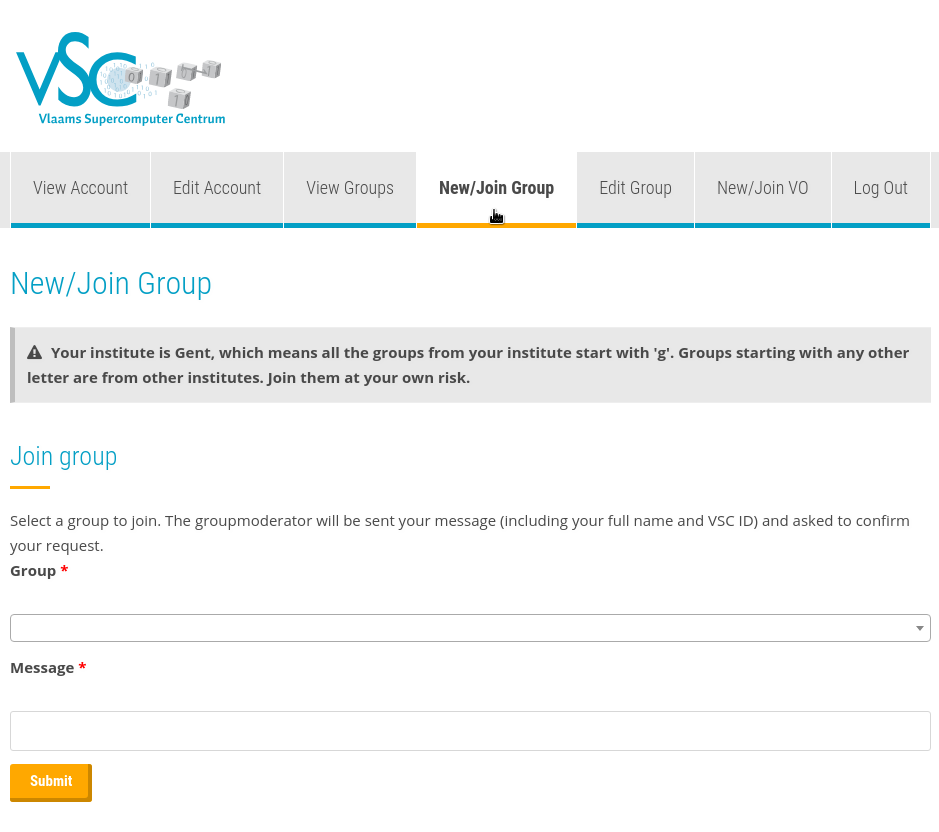
\includegraphics[width=\textwidth]{ch6-group-join}
\end{figure}\label{fig:group-join}

\subsection{Creating a new group}

\begin{enumerate}
    \item Go to \url{https://account.vscentrum.be/django/group/new} and scroll down
        to the section ``Request new group''. This should look something like
        \autoref{fig:group-new}.
    \item Fill out the group name. This cannot contain spaces.
    \item Put a description of your group in the ``Info'' field.
    \item You will now be a member and moderator of your newly created group.
\end{enumerate}

\begin{figure}[!htbp]
  \caption{Creating a new group.}
  \centering
    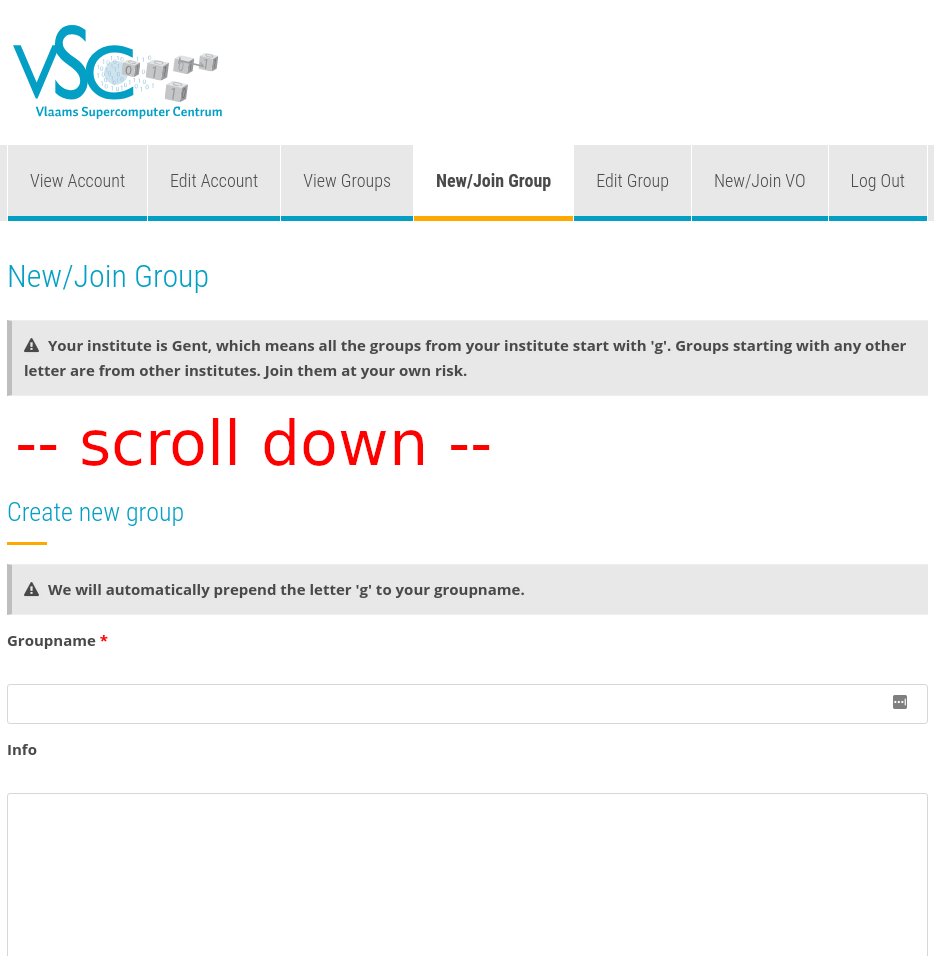
\includegraphics[width=\textwidth]{ch6-group-new}
\end{figure}\label{fig:group-new}

\subsection{Managing a group}

Group moderators can go to \url{https://account.vscentrum.be/django/group/edit} to
manage their group (see \autoref{fig:group-edit}). Moderators can invite and remove members. They can also promote
other members to moderator and remove other moderators.

\begin{figure}[!htbp]
  \caption{Creating a new group.}
  \centering
    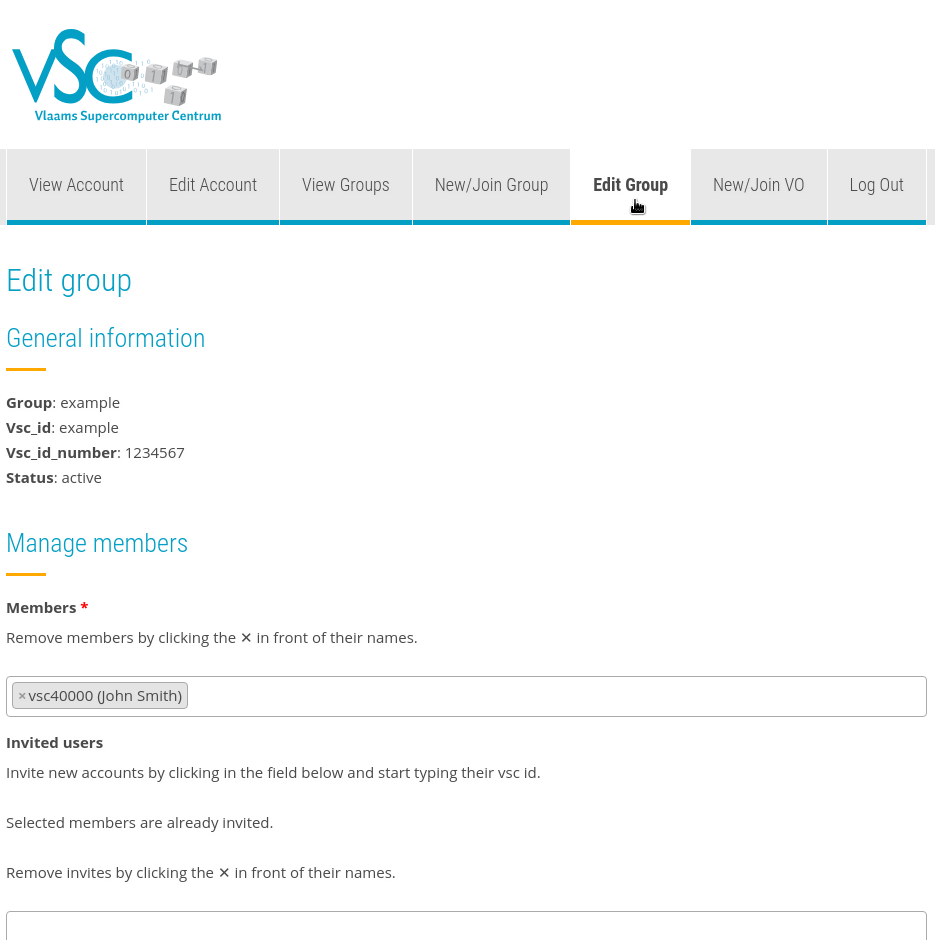
\includegraphics[width=\textwidth]{ch6-group-edit}
\end{figure}\label{fig:group-edit}

\subsection{Inspecting groups}

You can get details about the current state of groups on the HPC infrastructure
with the following command (\lstinline|example| is the name of the group we want to inspect):

\begin{prompt}
%\shellcmd{getent group example}%
example:*:1234567:vsc40001,vsc40002,vsc40003
\end{prompt}

We can see that the VSC id number is 1234567 and that there are three members in
the group: \lstinline|vsc40001|, \lstinline|vsc40002| and \lstinline|vsc40003|.

% virtual organisations are only used in Ghent (for now)
\ifgent
\section{Virtual Organisations}
\label{sec:virtual-organisations}
\hypertarget{sec:virtual-organisation}{}

A Virtual Organisation (VO) is a special type of group. You can only be a member
of one single VO at a time (or not be in a VO at all).
Being in a VO allows for larger storage quota to be obtained
(but these requests should be well-motivated).

\subsection{Joining an existing VO}

\begin{enumerate}
    \item Get the VO id of the research group you belong to (this id is formed by
        the letters \lstinline|gvo|, followed by 5 digits).
    \item Go to \url{https://account.vscentrum.be/django/vo/join} and fill in the
        section named ``Join VO''. You will be asked to fill in the VO id and a message for
        the moderator of the VO, where you identify yourself. This should look something
        like \autoref{fig:VO-join}.
    \item After clicking the submit button, a message will be sent to the moderator
    of the VO, who will either approve or deny the request.
\end{enumerate}



\begin{figure}[!htbp]
  \caption{Joining a VO.}
  \centering
    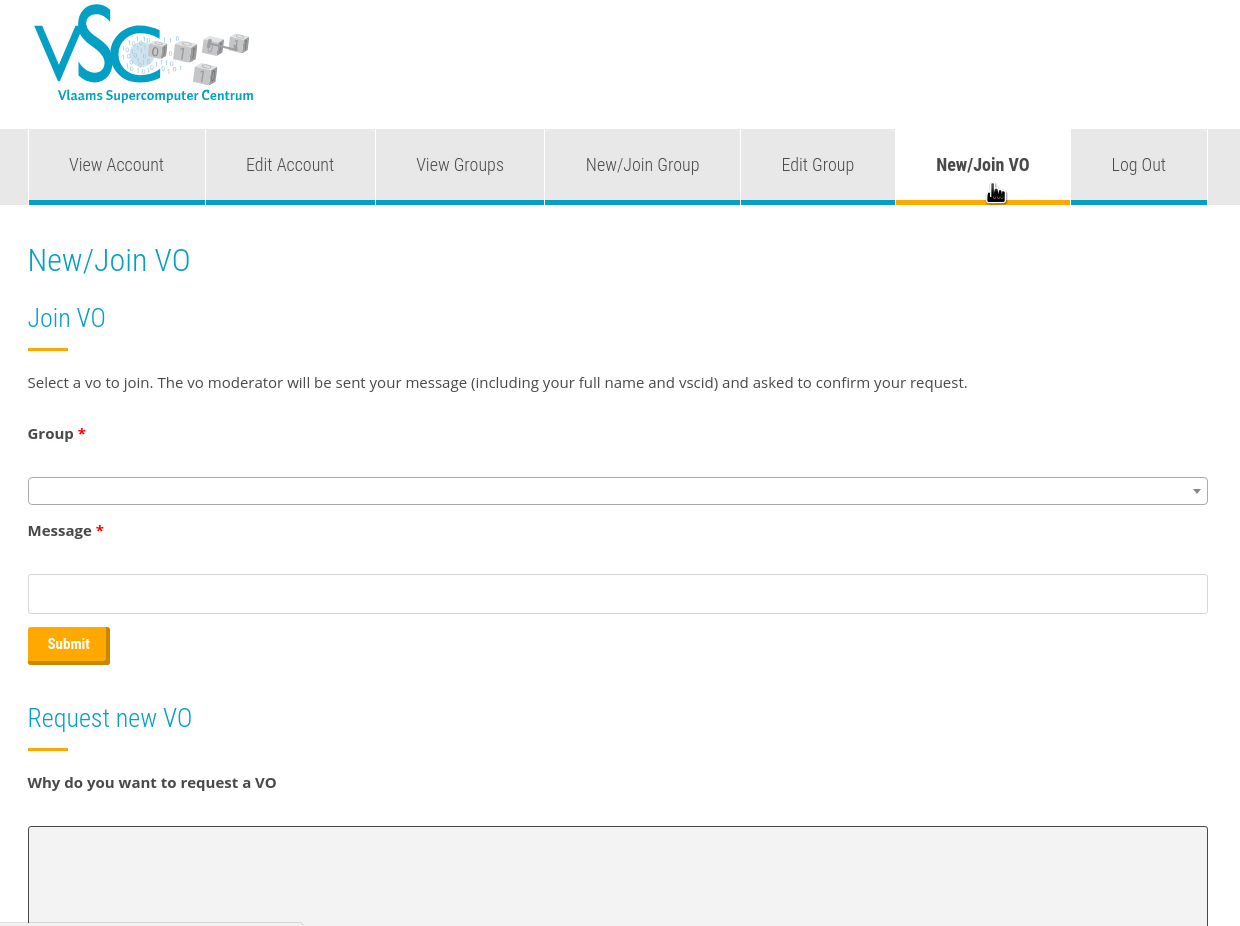
\includegraphics[width=\textwidth]{ch6-VO-join}
\end{figure}\label{fig:VO-join}

\subsection{Creating a new VO}

\begin{enumerate}
    \item Go to \url{https://account.vscentrum.be/django/vo/new} and scroll down
        to the section ``Request new VO''. This should look something like
        \autoref{fig:VO-new}.
    \item Fill why you want to request a VO.
    \item Fill out the both the internal and public VO name. These cannot contain
        spaces, and should be 8-10 characters long. For example, \lstinline|genome25| is
        a valid VO name.
    \item Fill out the rest of the form and press submit. This will send a message
        to the \hpc administrators, who will then either approve or deny the request.
    \item If the request is approved, you will now be a member and moderator of your
        newly created VO.
\end{enumerate}

\begin{figure}[!htbp]
  \caption{Creating a new VO.}
  \centering
    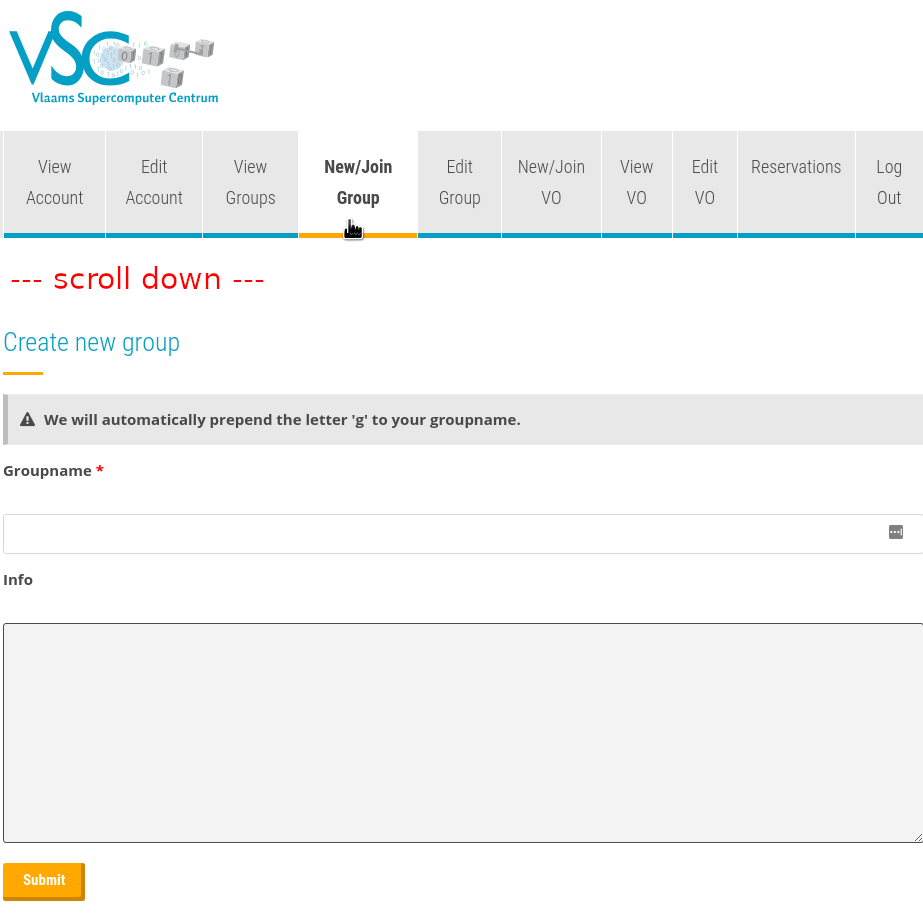
\includegraphics[width=\textwidth]{ch6-VO-new}
\end{figure}\label{fig:VO-new}

\subsection{Requesting more storage space}
\label{subsec:requesting-more-storage-space}

If you're a moderator of a VO, you can request additional quota for the VO and
its members.

\begin{enumerate}
    \item Go to \url{https://account.vscentrum.be/django/vo/edit} and scroll down
        to ``Request additional quota''. See \autoref{fig:VO-request-additional-quota} to see how this looks.
    \item Fill out how much \emph{additional} storage you want. In the screenshot below,
        we're asking for 500 GiB extra space for \lstinline|VSC_DATA|, and for 1 TiB extra
        space on \lstinline|VSC_SCRATCH_KYUKON|.
    \item Add a comment explaining why you need additional storage space and submit
        the form.
    \item An \hpc administrator will review your request and approve or deny it.
\end{enumerate}

\begin{figure}[!htbp]
  \caption{Requesting additional quota for the VO and its members.}
  \centering
    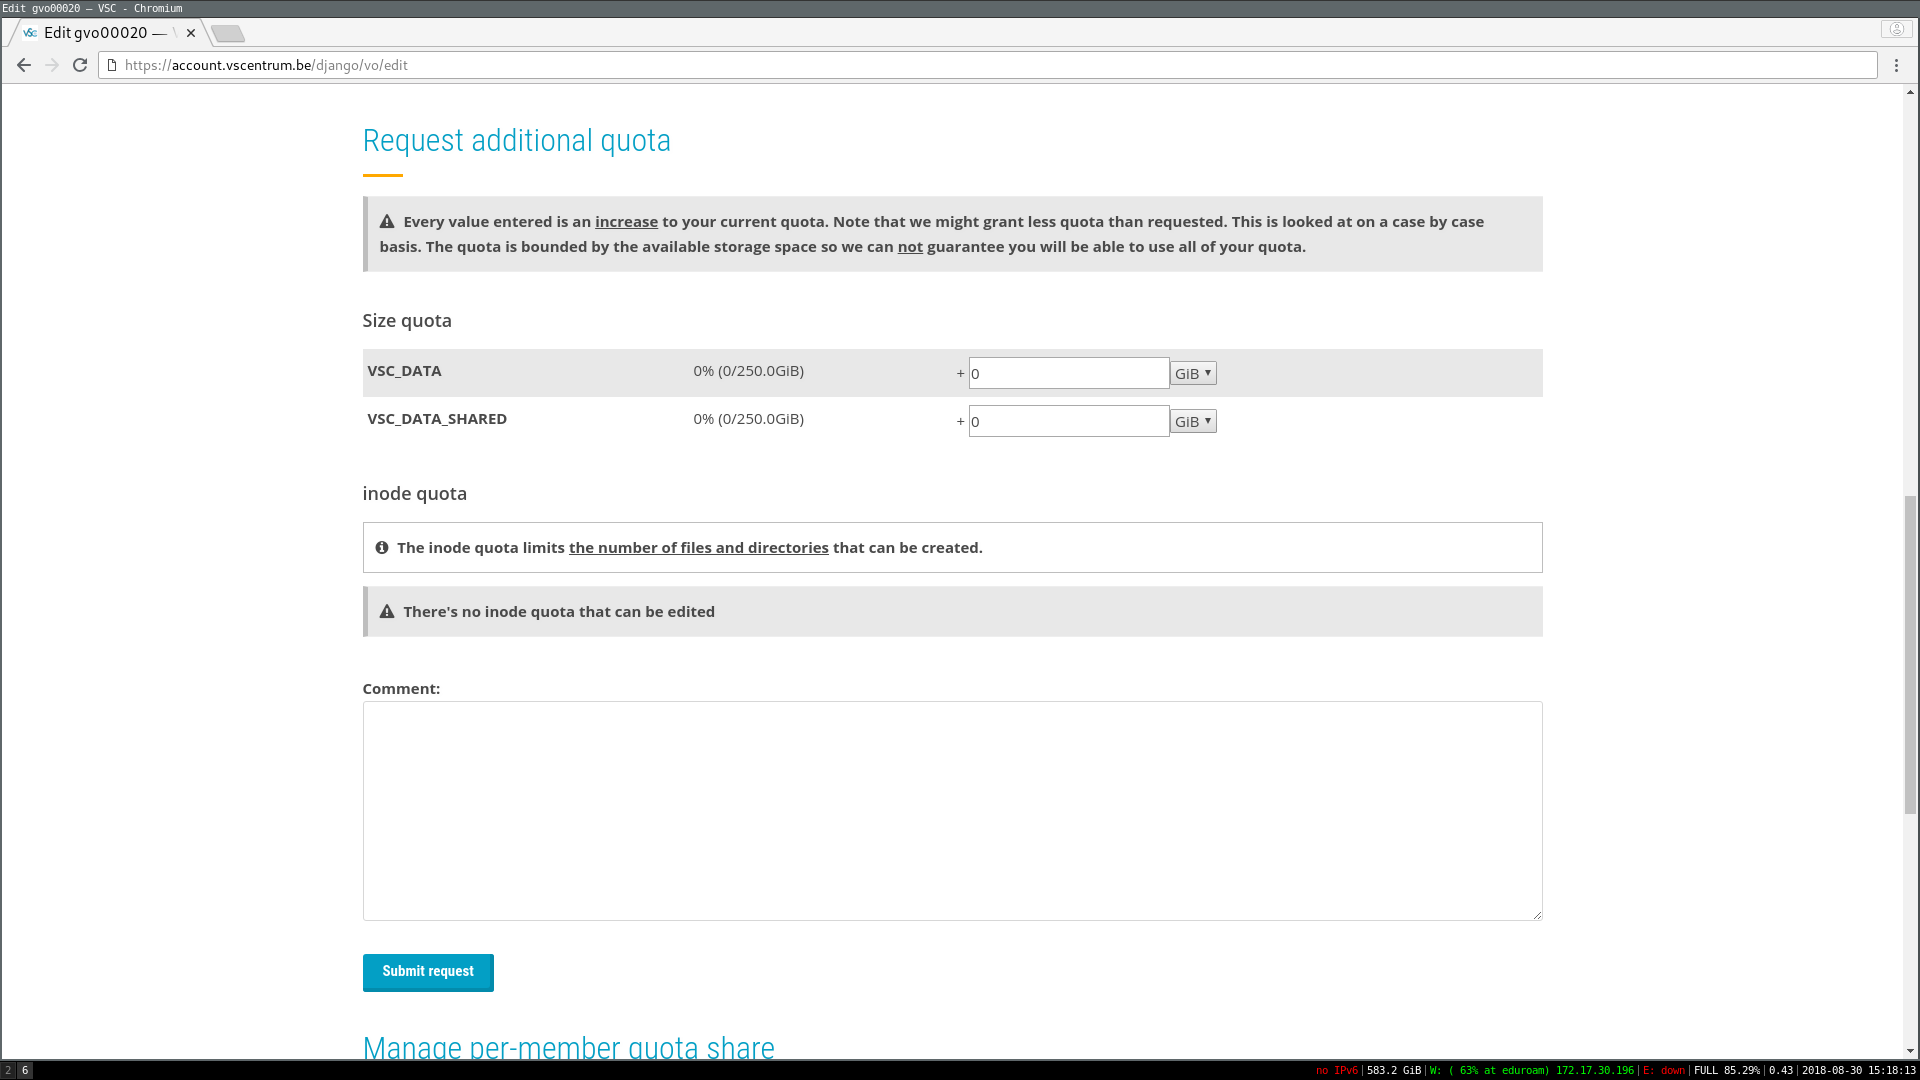
\includegraphics[width=\textwidth]{ch6-VO-request-additional-quota}
\end{figure}\label{fig:VO-request-additional-quota}

\subsection{Setting per-member VO quota}

VO moderators can tweak how much of the VO quota each member can use. By default,
this is set to 50\% for each user, but the moderator can change this: it is possible
to give a particular user more than half of the VO quota (for example 80\%), or
significantly less (for example 10\%).

Note that the total percentage can be above 100\%: the percentages the moderator
allocates per user are \emph{the maximum percentages} of storage users can use.

\begin{enumerate}
    \item Go to \url{https://account.vscentrum.be/django/vo/edit} and scroll down
        to ``Manage per-member quota share''. See \autoref{fig:VO-per-member-storage} to see how this looks.
    \item Fill out how much percent of the space you want each user to be able to use.
        Note that the total can be above 100\%. In the screenshot below, there are
        four users. Alice and Bob can use up to 50\% of the space, Carl
        can use up to 75\% of the space, and Dave can only use 10\% of the space.
        So in total, 185\% of the space has been assigned, but of course only
        100\% can actually be used.
\end{enumerate}

\begin{figure}[!htbp]
  \caption{Setting per-member quota.}
  \centering
    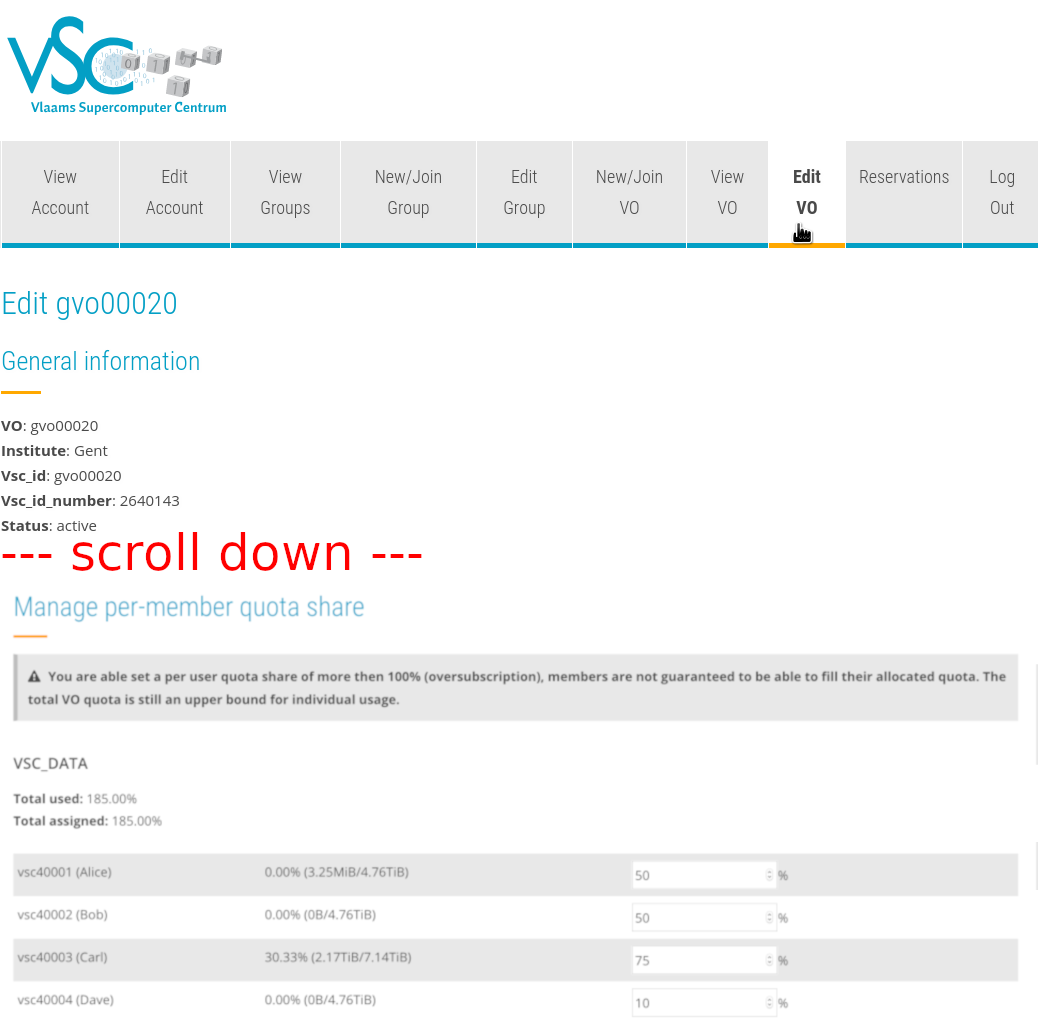
\includegraphics[width=\textwidth]{ch6-VO-per-member-storage}
\end{figure}\label{fig:VO-per-member-storage}

\subsection{VO directories}
\label{subsec:vo-directories}

When you're a member of a VO, there will be some additional directories
on each of the shared filesystems available:

\begin{description}
    \item[VO scratch (\texttt{\$VSC\_SCRATCH\_VO})]
        A directory on the shared \emph{scratch} filesystem shared by the members of your
        VO, where additional storage quota can be provided (see \autoref{subsec:requesting-more-storage-space}).
        You can use this as an alternative to your personal \lstinline|$VSC_SCRATCH|
        directory (see \autoref{subsec:scratch-directory}).

    \item[VO data (\texttt{\$VSC\_DATA\_VO})]
        A directory on the shared \emph{data} filesystem shared by the members of your
        VO, where additional storage quota can be provided (see \autoref{subsec:requesting-more-storage-space}).
        You can use this as an alternative to your personal \lstinline|$VSC_DATA|
        directory (see \autoref{subsec:data-directory}).

\end{description}

If you put \lstinline|_USER| after each of these variable names, you can see your
personal folder in these filesystems. For example: \lstinline|$VSC_DATA_VO_USER|
is your personal folder in your VO data filesystem (this is equivalent to
\lstinline|$VSC_DATA_VO/$USER|), and analogous for \lstinline|$VSC_SCRATCH_VO_USER|.

\fi


\chapter{Multi core jobs / Parallel Computing}

\section{Why Parallel Programming?}

There are two important motivations to engage in parallel programming.

\begin{enumerate}

\item  Firstly, the need to decrease the time to solution: distributing your
  code over \emph{C} cores holds the promise of speeding up execution times
  by a factor \emph{C}. All modern computers (and probably even your
  smartphone) are equipped with multi-core processors capable of parallel
  processing.
\item  The second reason is problem size: distributing your code over
  \emph{N} nodes increases the available memory by a factor \emph{N}, and
  thus holds the promise of being able to tackle problems which are \emph{N}
  times bigger.
\end{enumerate}

On a desktop computer, this enables a user to run multiple programs and the
operating system simultaneously. For scientific computing, this means you have
th ability in principle of splitting up your computations into groups and
running each group on its own core.

There are multiple different ways to achieve parallel programming. The table
below gives a (non-exhaustive) overview of problem independent approaches to
parallel programming. In addition there are many problem specific libraries
that incorporate parallel capabilities. The next three sections explore some
common approaches: (raw) threads, OpenMP and MPI.

\begin{tabular}{|p{0.15\textwidth}|p{0.3\textwidth}|p{0.55\textwidth}|} \hline
\multicolumn{3}{|c|}{\strong{Parallel programming approaches}} \\ \hline
\strong{Tool}                                                          & \strong{Available language bindings}                                   & \strong{Limitations} \\ \hline
Raw threads\newline pthreads, boost::\newline threading, \dots         & Threading libraries are available for all common programming languages & Threads are limited to a shared memory systems. They are more often used on single node systems rather than for UA-HPC. Thread management is hard. \\ \hline
OpenMP                                                                 & Fortran/C/C++                                                      & Limited to shared memory systems, but large shared memory systems for UA-HPC are not uncommon (e.g. SGI UV). Loops and task can be parallelized by simple insertion of compiler directives. Under the hood threads are used. Hybrid approaches exist which use OpenMP to parallelize the work load on each node and MPI (see below) for communication between nodes. \\ \hline
Lightweight threads with clever scheduling, Intel TBB, Intel Cilk Plus & C/C++                                                                & Limited to shared memory systems, but may be combined with MPI. Thread management is taken care of by a very clever scheduler enabling the programmer to focus on parallelization itself. Hybrid approaches exist which use TBB and/or Cilk Plus to parallelize the work load on each node and MPI (see below) for communication between nodes. \\ \hline
MPI                                                                    & Fortran/C/C++ Python                                             & Applies to both distributed and shared memory systems. Cooperation between different nodes or cores is managed by explicit calls to library routines handling communication routines. \\ \hline
Global Arrays library                                                  & C/C++ Python                                                       & Mimics a global address space on distributed memory systems, by distributing arrays over many nodes and one sided communication. This library is used a lot for chemical structure calculation codes and was used in one of the first applications that broke the PetaFlop barrier. \\ \hline
Scoop                                                                  & Python                                                                 & Applies to both shared and distributed memory system. Not extremely advanced, but may present a quick road to parallelization of python code.  \\ \hline
\end{tabular}

\section{Parallel Computing with threads}

Multi-threading is a widespread programming and execution model that allows
multiple threads to exist within the context of a single process. These threads
share the process' resources, but are able to execute independently. The
threaded programming model provides developers with a useful abstraction of
concurrent execution. Multi-threading can also be applied to a single process
to enable parallel execution on a multiprocessing system.

\includegraphics*[width=5.75in, height=2.39in, keepaspectratio=false]{img0700}

This advantage of a multithreaded program allows it to operate faster on
computer systems that have multiple CPUs or across a cluster of machines ---
because the threads of the program naturally lend themselves to truly
concurrent execution. In such a case, the programmer needs to be careful to
avoid race conditions, and other non-intuitive behaviors. In order for data to
be correctly manipulated, threads will often need to synchronize in time in
order to process the data in the correct order. Threads may also require
mutually exclusive operations (often implemented using semaphores) in order to
prevent common data from being simultaneously modified, or read while in the
process of being modified. Careless use of such primitives can lead to
deadlocks.

Threads are a way that a program can spawn concurrent units of processing that
can then be delegated by the operating system to multiple processing cores.
Clearly the advantage of a multithreaded program (one that uses multiple
threads that are assigned to multiple processing cores) is that you can achieve
big speedups, as all cores of your CPU (and all CPUs if you have more than one)
are used at the same time.

Here is a simple example program that spawns 7 threads, where each one runs a
simple function that only prints ``Hello from thread''.

Go to the example directory:

\begin{prompt}
%\shellcmd{cd \tilde/\exampledir}%
\end{prompt}

Study the example first:

\examplecode{C}{T_hello.c}

And compile it (whilst including the thread library) and run and test it on the login-node:

\begin{prompt}
%\shellcmd{module load GCC}%
%\shellcmd{gcc -o T\_hello T\_hello.c -lpthread}%
%\shellcmd{./T\_hello}%
spawning thread 0
spawning thread 1
spawning thread 2
Hello from thread 0!
Hello from thread 1!
Hello from thread 2!
spawning thread 3
spawning thread 4
Hello from thread 3!
Hello from thread 4!
\end{prompt}

Now, run it on the cluster and check the output:

\begin{prompt}
%\shellcmd{qsub T\_hello.pbs}%
%\jobid%
%\shellcmd{more T\_hello.pbs.o\jobnumber}%
spawning thread 0
spawning thread 1
spawning thread 2
Hello from thread 0!
Hello from thread 1!
Hello from thread 2!
spawning thread 3
spawning thread 4
Hello from thread 3!
Hello from thread 4!
\end{prompt}

% FIXME: Refer to Hager & co insted of this.
\underbar{Tip:} If you plan engaging in parallel programming using threads,
this book may prove useful: \emph{Professional Multicore Programming: Design
and Implementation for C++ Developers. Cameron Hughes and Tracey Hughes. Wrox
2008.}

\section{Parallel Computing with OpenMP}

\strong{\emph{OpenMP}} is an API that implements a multi-threaded, shared
memory form of parallelism. It uses a set of compiler directives (statements
that you add to your code and that are recognized by your Fortran/C/C++
compiler if OpenMP is enabled or otherwise ignored) that are incorporated at
compile-time to generate a multi-threaded version of your code. You can think
of Pthreads (above) as doing multi-threaded programming "by hand", and OpenMP
as a slightly more automated, higher-level API to make your program
multithreaded. OpenMP takes care of many of the low-level details that you
would normally have to implement yourself, if you were using Pthreads from the
ground up.

An important advantage of OpenMP is that, because it uses compiler directives,
the original serial version stays intact, and minimal changes (in the form of
compiler directives) are necessary to turn a working serial code into a working
parallel code.

Here is the general code structure of an OpenMP program:

\begin{code}{C}
#include <omp.h>
main ()  {
int var1, var2, var3;
Serial code
%\dots%
Beginning of parallel section. Fork a team of threads.
Specify variable scoping

#pragma omp parallel private(var1, var2) shared(var3)
  {
  Parallel section executed by all threads
  All threads join master thread and disband
  }
Resume serial code
}
\end{code}

\subsection{Private versus Shared variables}

By using the private() and shared() clauses, you can specify variables within
the parallel region as being \strong{shared}, i.e. visible and accessible by
all threads simultaneously, or \strong{private}, i.e. private to each thread,
meaning each thread will have its own local copy. In the code example below for
parallelizing a for loop, you can see that we specify the thread\_id and nloops
variables as private.

\subsection{Parallelizing for loops with OpenMP}

Parallelizing for loops is really simple (see code below). By default, loop
iteration counters in OpenMP loop constructs (in this case the i variable) in
the for loop are set to private variables.

\examplecode{C}{omp1.c}

And compile it (whilst including the ``\emph{openmp}'' library) and run and test it on the login-node:

\begin{prompt}
%\shellcmd{module load GCC}%
%\shellcmd{gcc -fopenmp -o omp1 omp1.c}%
%\shellcmd{./omp1}%
Thread 6 performed 125 iterations of the loop.
Thread 7 performed 125 iterations of the loop.
Thread 5 performed 125 iterations of the loop.
Thread 4 performed 125 iterations of the loop.
Thread 0 performed 125 iterations of the loop.
Thread 2 performed 125 iterations of the loop.
Thread 3 performed 125 iterations of the loop.
Thread 1 performed 125 iterations of the loop.
\end{prompt}

Now run it in the cluster and check the result again.

\begin{prompt}
%\shellcmd{qsub omp1.pbs}%
%\shellcmd{cat omp1.pbs.o*}%
Thread 1 performed 125 iterations of the loop.
Thread 4 performed 125 iterations of the loop.
Thread 3 performed 125 iterations of the loop.
Thread 0 performed 125 iterations of the loop.
Thread 5 performed 125 iterations of the loop.
Thread 7 performed 125 iterations of the loop.
Thread 2 performed 125 iterations of the loop.
Thread 6 performed 125 iterations of the loop.
\end{prompt}

\subsection{Critical Code}

Using OpenMP you can specify something called a "critical" section of code.
This is code that is performed by all threads, but is only performed
\strong{one thread at a time} (i.e. in serial). This provides a convenient way
of letting you do things like updating a global variable with local results
from each thread, and you don't have to worry about things like other threads
writing to that global variable at the same time (a collision).

\examplecode{C}{omp2.c}

And compile it (whilst including the ``\emph{openmp}'' library) and run and test it on the login-node:

\begin{prompt}
%\shellcmd{module load GCC}%
%\shellcmd{gcc -fopenmp -o  omp2   omp2.c}%
%\shellcmd{./omp2}%
Thread 3 is adding its iterations (12500) to sum (0), total is now 12500.
Thread 7 is adding its iterations (12500) to sum (12500), total is now 25000.
Thread 5 is adding its iterations (12500) to sum (25000), total is now 37500.
Thread 6 is adding its iterations (12500) to sum (37500), total is now 50000.
Thread 2 is adding its iterations (12500) to sum (50000), total is now 62500.
Thread 4 is adding its iterations (12500) to sum (62500), total is now 75000.
Thread 1 is adding its iterations (12500) to sum (75000), total is now 87500.
Thread 0 is adding its iterations (12500) to sum (87500), total is now 100000.
Total # loop iterations is 100000
\end{prompt}

Now run it in the cluster and check the result again.

\begin{prompt}
%\shellcmd{qsub omp2.pbs}%
%\shellcmd{cat omp2.pbs.o*}%
Thread 2 is adding its iterations (12500) to sum (0), total is now 12500.
Thread 0 is adding its iterations (12500) to sum (12500), total is now 25000.
Thread 1 is adding its iterations (12500) to sum (25000), total is now 37500.
Thread 4 is adding its iterations (12500) to sum (37500), total is now 50000.
Thread 7 is adding its iterations (12500) to sum (50000), total is now 62500.
Thread 3 is adding its iterations (12500) to sum (62500), total is now 75000.
Thread 5 is adding its iterations (12500) to sum (75000), total is now 87500.
Thread 6 is adding its iterations (12500) to sum (87500), total is now 100000.
Total # loop iterations is 100000
\end{prompt}

\subsection{Reduction}

Reduction refers to the process of combining the results of several
sub-calculations into a final result. This is a very common paradigm (and
indeed the so-called "map-reduce" framework used by Google and others is very
popular). Indeed we used this paradigm in the code example above, where we used
the "critical code" directive to accomplish this. The map-reduce paradigm is so
common that OpenMP has a specific directive that allows you to more easily
implement this.

\examplecode{C}{omp3.c}

And compile it (whilst including the ``\emph{openmp}'' library) and run and
test it on the login-node:

\begin{prompt}
%\shellcmd{gcc -fopenmp -o omp3 omp3.c}%
%\shellcmd{./omp3}%
Total # loop iterations is 100000
\end{prompt}

Now run it in the cluster and check the result again.

\begin{prompt}
%\shellcmd{qsub omp3.pbs}%
%\shellcmd{cat omp3.pbs.o*}%
Total # loop iterations is 100000
\end{prompt}

\subsection{Other OpenMP directives}

There are a host of other directives you can issue using OpenMP.

Some other clauses of interest are:

\begin{enumerate}
\item  barrier: each thread will wait until all threads have reached this point in the code, before proceeding
\item  nowait: threads will not wait until everybody is finished
\item  schedule(type, chunk) allows you to specify how tasks are spawned out to threads in a for loop. There are three types of scheduling you can specify
\item  if: allows you to parallelize only if a certain condition is met
\item  \dots  and a host of others
\end{enumerate}

\underbar{Tip:} If you plan engaging in parallel programming using OpenMP, this
book may prove useful: \textit{Using OpenMP - Portable Shared Memory Parallel
Programming}. By Barbara Chapman Gabriele Jost and Ruud van der Pas Scientific
and Engineering Computation. 2005.

\section{Parallel Computing with MPI }

The Message Passing Interface (MPI) is a standard defining core syntax and
semantics of library routines that can be used to implement parallel
programming in C (and in other languages as well). There are several
implementations of MPI such as Open MPI, Intel MPI, M(VA)PICH(2) and LAM/MPI.

In the context of this tutorial, you can think of MPI, in terms of its
complexity, scope and control, as sitting in between programming with Pthreads,
and using a high-level API such as OpenMP. For a Message Passing Interface
(MPI) application, a parallel task usually consists of a single executable
running concurrently on multiple processors, with communication between the
processes.  This is shown in the following diagram:

\includegraphics*[width=1.50in, height=1.59in, keepaspectratio=false]{img0701}

The process numbers 0, 1 and 2 represent the process rank and have greater or
less significance depending on the processing paradigm. At the minimum, Process
0 handles the input/output and determines what other processes are running.

The MPI interface allows you to manage allocation, communication, and
synchronization of a set of processes that are mapped onto multiple nodes,
where each node can be a core within a single CPU, or CPUs within a single
machine, or even across multiple machines (as long as they are networked
together).

One context where MPI shines in particular is the ability to easily take
advantage not just of multiple cores on a single machine, but to run programs
on clusters of several machines. Even if you don't have a dedicated cluster,
you could still write a program using MPI that could run your program in
parallel, across any collection of computers, as long as they are networked
together. Just make sure to ask permission before you load up your lab-mate's
computer's CPU(s) with your computational tasks!

Here is a "Hello World" program in MPI written in C. In this example, we send a
"Hello" message to each processor, manipulate it trivially, return the results
to the main process, and print the messages.

Study the MPI-programme and the PBS-file:

\examplecode{C}{mpi_hello.c}
\examplecode{bash}{mpi_hello.pbs}

mpiicc is a wrapper of the Intel C++ compiler icc to compile MPI programs (see
the chapter on compilation for details).

Run the parallel program:

\begin{prompt}
%\shellcmd{qsub mpi\_hello.pbs}%
%\shellcmd{ls -l}%
total 1024
-rwxrwxr-x 1 %\userid% 8746 Sep 16 14:19 mpi_hello*
-rw-r--r-- 1 %\userid% 1626 Sep 16 14:18 mpi_hello.c
-rw------- 1 %\userid%    0 Sep 16 14:22 mpi_hello.o%\jobnumber%
-rw------- 1 %\userid%  697 Sep 16 14:22 mpi_hello.o%\jobnumber%
-rw-r--r-- 1 %\userid%  304 Sep 16 14:22 mpi_hello.pbs
%\shellcmd{cat mpi\_hello.o\jobnumber}%
0: We have 16 processors
0: Hello 1! Processor 1 reporting for duty
0: Hello 2! Processor 2 reporting for duty
0: Hello 3! Processor 3 reporting for duty
0: Hello 4! Processor 4 reporting for duty
0: Hello 5! Processor 5 reporting for duty
0: Hello 6! Processor 6 reporting for duty
0: Hello 7! Processor 7 reporting for duty
0: Hello 8! Processor 8 reporting for duty
0: Hello 9! Processor 9 reporting for duty
0: Hello 10! Processor 10 reporting for duty
0: Hello 11! Processor 11 reporting for duty
0: Hello 12! Processor 12 reporting for duty
0: Hello 13! Processor 13 reporting for duty
0: Hello 14! Processor 14 reporting for duty
0: Hello 15! Processor 15 reporting for duty
\end{prompt}

The runtime environment for the MPI implementation used (often called mpirun or
mpiexec) spawns multiple copies of the program, with the total number of copies
determining the number of process \emph{ranks} in MPI\_COMM\_WORLD, which is
an opaque descriptor for communication between the set of processes. A single
process, multiple data (SPMD = Single Program, Multiple Data) programming model
is thereby facilitated, but not required; many MPI implementations allow
multiple, different, executable's to be started in the same MPI job. Each
process has its own rank, the total number of processes in the world, and the
ability to communicate between them either with point-to-point (send/receive)
communication, or by collective communication among the group. It is enough for
MPI to provide an SPMD-style program with MPI\_COMM\_WORLD, its own rank, and
the size of the world to allow algorithms to decide what to do. In more
realistic situations, I/O is more carefully managed than in this example. MPI
does not guarantee how POSIX I/O would actually work on a given system, but it
commonly does work, at least from rank 0.

MPI uses the notion of process rather than processor. Program copies are
\emph{mapped} to processors by the MPI runtime. In that sense, the parallel
machine can map to 1 physical processor, or N where N is the total number of
processors available, or something in between. For maximum parallel speedup,
more physical processors are used. This example adjusts its behavior to the
size of the world N, so it also seeks to scale to the runtime configuration
without compilation for each size variation, although runtime decisions might
vary depending on that absolute amount of concurrency available.


\underbar{Tip:} If you plan engaging in parallel programming using MPI, this
book may prove useful: \emph{Parallel Programming with MPI. Peter Pacheo.
Morgan Kaufmann. 1996.}


\chapter{Troubleshooting}
\label{ch:troubleshooting}



\section{Walltime issues}
If you get from your job output an error message similar to this:

\begin{prompt}
 =>> PBS: job killed: walltime %\emph{<value in seconds>}% exceeded limit %\emph{<value in seconds>}%
\end{prompt}

This occurs when your job did not complete within the requested walltime.
See section~\ref{sec:specifying-walltime-requirements} for more information about how to request the walltime.
It is recommended to use \emph{checkpointing} if the job requires \strong{72 hours} of walltime or more to be executed.
% FIXME: Refer to Checkpointing section.



\section{Out of quota issues}

Sometimes a job hangs at some point or it stops writing in the disk. These errors are usually
related to the quota usage. You may have reached your quota limit at some storage endpoint.
You should move (or remove) the data to a different storage endpoint (or request more quota) to be able to write to the disk and then resubmit the jobs.
\ifgent
Another option is to request extra quota for your VO to the VO moderator/s.
See section~\ref{subsec:predefined-user-directories} and section~\ref{subsec:predfined-quotas} for more information about
quotas and how to use the storage endpoints in an efficient way.
\fi
% FIXME: Add how to request quota section

\section{Issues connecting to login node}
\label{sec:connecting-issues}

If you are confused about the SSH public/private key pair concept, maybe the
key/lock analogy in \autoref{subsec:how-do-ssh-keys-work} can help.

If you have errors that look like:

\begin{prompt}
%\userid{}%@%\loginnode{}%: Permission denied
\end{prompt}

or you are experiencing problems with connecting, here is a list of things to do
that should help:

\begin{enumerate}
    \item Keep in mind that it an take up to an hour for your VSC account to become
        active after it has been \emph{approved}; until then, logging in to your VSC
        account will not work.
    \item Make sure you are connecting from an IP address that is allowed to access the VSC login nodes,
          see section~\ref{sec:connection-restrictions} for more information.
\ifmacORlinux
    \item Your SSH private key may not be in the default location (\lstinline|$HOME/.ssh/id_rsa|).
        There are several ways to deal with this (using one of these is sufficient):
\begin{enumerate}
            \item Use the \lstinline|ssh -i| (see section~\ref{sec:connect}) \emph{OR;}
            \item Use \lstinline|ssh-add| (see section~\ref{sec:using-ssh-agent-with-openssh}) \emph{OR;}
            \item Specify the location of the key in \lstinline|$HOME/.ssh/config|. You will
                need to replace the VSC login id in the \lstinline|User| field with your own:

            \begin{prompt}
Host %\hpcname{}%
    Hostname %\loginnode{}%
    IdentityFile %\emph{/path/to/private/key}%
    User %\emph{\userid{}}%\end{prompt}

    Now you can just connect with \texttt{ssh \hpcname}.
\end{enumerate}
\fi
        \item Please double/triple check your VSC login ID. It should look
            something like \emph{\userid}: the letters \lstinline|vsc|, followed
            by exactly 5 digits. Make sure it's the same one as the one on
            \url{https://account.vscentrum.be/}.
        \item You previously connected to the \hpc from another machine, but now
            have another machine? Please follow the procedure for adding additional
            keys in section~\ref{sec:adding-multiple-keys}. You may need to wait
            for 15-20 minutes until the SSH public key(s) you added become active.
        \item \ifwindows Make sure you are using the private key (not the public key) when trying to connect:
            If you followed the manual, the private key filename should end in
            \lstinline|.ppk| (not in \lstinline|.pub|).
            \else
            When using an SSH key in a non-default location, make sure you supply
            the path of the private key (and not the path of the public key)
            to \lstinline|ssh|. \lstinline|id_rsa.pub| is the usual filename of the public
            key, \lstinline|id_rsa| is the usual filename of the private key.
            (See also section~\ref{sec:connect})
            \fi
        \item If you have multiple private keys on your machine, please make sure
            you are using the one that corresponds to (one of) the public key(s) you
            added on \url{https://account.vscentrum.be/}.
        \item Please do not use someone else's private keys. You must never
            share your private key, they're called \emph{private} for a good reason.
\end{enumerate}

\ifwindows

If you are using PuTTY and get this error message:

\begin{prompt}
server unexpectedly closed network connection
\end{prompt}

it is possible that the PuTTY version you are using is too old and doesn't
support some required (security-related) features.

Make sure you are using the latest PuTTY version if you are encountering problems
connecting (see \autoref{sec:install-putty}). If that doesn't help, please contact \hpcinfo.

\fi

If you've tried all applicable items above and it doesn't solve your problem,
please contact \hpcinfo and include the following information:

\ifwindows
Please create a log file of your SSH session by following the steps
in \href{https://my.kualo.com/knowledgebase/?kbcat=0&article=888}{this article}
and include it in the email.

\subsection{Change PuTTY private key for a saved configuration}
\label{subsec:putty-change-key}

\newcounter{puttyenum}
\begin{enumerate}
    \item Open PuTTY

    \item Single click on the saved configuration

    \begin{center}
    \includegraphics*[width=2.49in, keepaspectratio=true]{831change01}
    \end{center}

    \item Then click \keys{Load} button

    \begin{center}
    \includegraphics*[width=2.49in, keepaspectratio=true]{831change02}
    \end{center}

    \item Expand SSH category (on the left panel) clicking on the "+" next to SSH

    \begin{center}
    \includegraphics*[width=2.49in, keepaspectratio=true]{831change03}
    \end{center}

    \item \label{item:putty-auth-ssh} \setcounter{puttyenum}{\value{enumi}} Click on Auth under the SSH category

    \begin{center}
    \includegraphics*[width=2.49in, keepaspectratio=true]{831change04}
    \end{center}

    \item On the right panel, click \keys{Browse} button

    \begin{center}
    \includegraphics*[width=2.49in, keepaspectratio=true]{831change05}
    \end{center}

    \item Then search your private key on your computer (with the extension ``.ppk'')

    \item Go back to the top of category, and click Session

    \begin{center}
    \includegraphics*[width=2.49in, keepaspectratio=true]{831change06}
    \end{center}

    \item On the right panel, click on \keys{Save} button

    \begin{center}
    \includegraphics*[width=2.49in, keepaspectratio=true]{831change07}
    \end{center}
\end{enumerate}

\subsection{Check whether your private key in PuTTY matches the public key on the accountpage}

Follow the instructions in \autoref{subsec:putty-change-key} util item \autoref{item:putty-auth-ssh}, then:
\begin{enumerate}
    \setcounter{enumi}{\value{puttyenum}}
    \item Single click on the textbox containig the path to your private key, then select all text
        (push \keys{Ctrl} + \keys{a}), then copy the location of the private key (push \keys{Ctrl} + \keys{c})

    \begin{center}
    \includegraphics*[width=2.49in, keepaspectratio=true]{832check05}
    \end{center}

    \item Open PuTTYgen

    \begin{center}
    \includegraphics*[width=2.49in, keepaspectratio=true]{832check06}
    \end{center}

    \item Enter menu item "File" and select "Load Private key"

    \begin{center}
    \includegraphics*[width=2.49in, keepaspectratio=true]{832check07}
    \end{center}

    \item On the "Load private key" popup, click in the textbox next to "File name:", then paste the location of
        your private key (push \keys{Ctrl} + \keys{v}), then click \keys{Open}

    \begin{center}
    \includegraphics*[width=5.21in, keepaspectratio=true]{832check08}
    \end{center}

    \item Make sure that your Public key from the "Public key for pasting into OpenSSH authorized\_keys file"
        textbox is in your "Public keys" section on the accountpage \url{https://account.vscentrum.be}.
        (Scroll down to the bottom of "View Account" tab, you will find there the "Public keys" section)

    \begin{center}
    \includegraphics*[width=2.49in,  keepaspectratio=true]{832check09}
    \end{center}
\end{enumerate}

\else
Please add \lstinline|-vvv| as a flag to \lstinline|ssh| like:

\begin{prompt}
%\shellcmd{ssh -vvv \userid{}@\loginnode{}}%
\end{prompt}

and include the output of that command in the message.
\fi

\section{Security warning about invalid host key}
\label{sec:security-warning-invald-host-key}

If you get a warning that looks like the one below, it is possible
that someone is trying to intercept the connection between you and the system you are connecting to.
Another possibility is that the host key of the system you are connecting to has changed.

\ifmacORlinux

\begin{prompt}
@@@@@@@@@@@@@@@@@@@@@@@@@@@@@@@@@@@@@@@@@@@@@@@@@@@@@@@@@@@
@    WARNING: REMOTE HOST IDENTIFICATION HAS CHANGED!     @
@@@@@@@@@@@@@@@@@@@@@@@@@@@@@@@@@@@@@@@@@@@@@@@@@@@@@@@@@@@
IT IS POSSIBLE THAT SOMEONE IS DOING SOMETHING NASTY!
Someone could be eavesdropping on you right now (man-in-the-middle attack)!
It is also possible that a host key has just been changed.
The fingerprint for the ECDSA key sent by the remote host is
SHA256:C8TVx0w8UjGgCQfCmEUaOPxJGNMqv2PXLyBNODe5eOQ.
Please contact your system administrator.
Add correct host key in ~/.ssh/known_hosts to get rid of this message.
Offending ECDSA key in ~/.ssh/known_hosts:%\strong{21}%
ECDSA host key for %\loginnode{}% has changed and you have requested strict checking.
Host key verification failed.
\end{prompt}

You will need to remove the line it's complaining about (in the example, line 21).
To do that, open \lstinline|~/.ssh/config| in an editor, and remove the line. This
results in \lstinline|ssh| ``forgetting'' the system you are connecting to.

After you've done that, you'll need to connect to the \hpc again.
See \autoref{sec:warning-message-new-host} to verify the fingerprints.
\strong{It's important to verify the fingerprints. If they don't match,
do \emph{not} connect and contact \hpcinfo instead.}

\else

You will need to verify that the fingerprint shown in the dialog matches one of the
following fingerprints:

\puttyFirstConnect

\strong{Do not click ``Yes'' until you verified the fingerprint. Do not press ``No'' in any case.}.

If it the fingerprint matches, click ``Yes''.

If it doesn't (like in the example) or you are in doubt, take a screenshot, press ``Cancel'' and contact \hpcinfo.

\sshedfingerprintnote

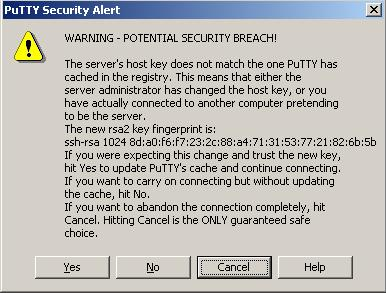
\includegraphics[width=0.5\textwidth]{putty_security_alert}


\fi


\section{DOS/Windows text format}

If you get errors like:

\begin{prompt}
%\shellcmd{qsub fibo.pbs}%
qsub:  script is written in DOS/Windows text format
\end{prompt}

It's probably because you transferred the files from a Windows computer.
Please go to the section about \lstinline|dos2unix| in \href{\LinuxManualURL#sec:dos2unix}{chapter 5 of the intro to Linux}
to fix this error.

\section{Warning message when first connecting to new host}
\label{sec:warning-message-new-host}

\ifmacORlinux
\begin{prompt}
%\shellcmd{ssh \userid{}@\loginnode{}}%
The authenticity of host %\loginnode{}% (<IP-adress>) can't be established.
%\underline{<algorithm> key fingerprint is <hash>}%
Are you sure you want to continue connecting (yes/no)?
\end{prompt}

Now you can check the authenticity by checking if the line that is at the place
of the underlined piece of text matches one of the following lines:
\begin{prompt}
%\opensshFirstConnect{}%
\end{prompt}

If it does, type  \strong{\emph{yes}}. If it doesn't, please contact support: \hpcinfo.

\else
\firsttimeconnection
\fi

\section{Memory limits}

To avoid jobs allocating too much memory, there are memory limits in place by default.
It is possible to specify higher memory limits if your jobs require this.

\subsection{How will I know if memory limits are the cause of my problem?}

If your program fails with a memory-related issue, there is a good chance it failed
because of the memory limits and you should increase the memory limits for your job.

Examples of these error messages are: \lstinline|malloc failed|, \lstinline|Out of memory|,
\lstinline|Could not allocate memory|
or in Java: \lstinline|Could not reserve enough space for object heap|. Your program can
also run into a \lstinline|Segmentation fault| (or \lstinline|segfault|) or crash due to bus errors.

You can check the amount of virtual memory (in Kb) that is available to you via the
\lstinline|ulimit -v| command \emph{in your job script}.

\subsection{How do I specify the amount of memory I need?}

See \autoref{subsec:generic-resource-requirements} to set memory and other requirements,
see \autoref{sec:specifying-memory-requirements} to finetune the amount of memory you request.
% See issue #248 to fix Java. This is software specific.
% See issue #196 to fix MATLAB. This is software specific.

\ifgent

\section{Module conflicts}
\label{sec:module-conflicts}

Modules that are loaded together must use the same toolchain version:
it is impossible to load two versions of the same module. In the following
example, we try to load a module that uses the \lstinline|intel-2018a| toolchain
together with one that uses the \lstinline|intel-2017a| toolchain:

\begin{prompt}
%\shellcmd{module load Python/2.7.14-intel-2018a}%
%\shellcmd{module load  HMMER/3.1b2-intel-2017a}%
Lmod has detected the following error:  A different version of the 'intel' module is already loaded (see output of 'ml').
You should load another 'HMMER' module for that is compatible with the currently loaded version of 'intel'.
Use 'ml avail HMMER' to get an overview of the available versions.

If you don't understand the warning or error, contact the helpdesk at hpc@ugent.be
While processing the following module(s):

    Module fullname          Module Filename
    ---------------          ---------------
    HMMER/3.1b2-intel-2017a  /apps/gent/CO7/haswell-ib/modules/all/HMMER/3.1b2-intel-2017a.lua
\end{prompt}

This resulted in an error because we tried to load two different versions of the
\lstinline|intel| module.

To fix this, check if there are other versions of the modules you want to load
that have the same version of common dependencies. You can list all versions of
a module with \lstinline|module avail|: for \lstinline|HMMER|, this command is \lstinline|module avail HMMER|.

Another common error is:

\begin{prompt}
%\shellcmd{module load cluster/\othercluster{}}%
Lmod has detected the following error:  A different version of the 'cluster' module is already loaded (see output of 'ml').

If you don't understand the warning or error, contact the helpdesk at hpc@ugent.be
\end{prompt}

This is because there can only be one \lstinline|cluster| module active at a time.
The correct command is \texttt{module \emph{swap} cluster/\othercluster}. See
also \autoref{subsec:specifying-the-cluster-on-which-to-run}.
\fi

\ifgent

\section{Running software that is incompatible with host}
\label{sec:running-software-incompatible-with-host}

When running software provided through modules (see \autoref{sec:modules}),
you may run into errors like:

\begin{prompt}
%\shellcmd{module swap cluster/kirlia}%

The following have been reloaded with a version change:
  1) cluster/victini => cluster/kirlia

%\shellcmd{module load Python/2.7.14-intel-2018a}%
%\shellcmd{python}%

Please verify that both the operating system and the processor support Intel(R) MOVBE, F16C, FMA, BMI, LZCNT and AVX2 instructions.

\end{prompt}

or errors like:

\begin{prompt}
%\shellcmd{module swap cluster/doduo}%

The following have been reloaded with a version change:
  1) cluster/victini => cluster/doduo

%\shellcmd{module load Python/2.7.14-foss-2018a}%
%\shellcmd{python}%
Illegal instruction
\end{prompt}


When we swap to a different cluster, the available modules change so they work for that cluster.
That means that if the cluster and the login nodes have a different CPU architecture,
software loaded using modules might not work.

If you want to test software on the login nodes, make sure the \texttt{cluster/\defaultcluster}
module is loaded (with \texttt{module swap cluster/\defaultcluster}, see
\autoref{subsec:specifying-the-cluster-on-which-to-run}),
since the login nodes and \defaultcluster have the same CPU architecture.

If modules are already loaded, and then we swap to a different cluster,
all our modules will get reloaded. This means that all current modules will be
unloaded and then loaded again, so they'll work on the newly loaded cluster.
Here's an example of how that would look like:

\begin{prompt}
%\shellcmd{module load Python/2.7.14-intel-2018a}%
%\shellcmd{module swap cluster/swalot}%

Due to MODULEPATH changes, the following have been reloaded:
  1) GCCcore/6.4.0                   5) Tcl/8.6.8-GCCcore-6.4.0           9) iccifort/2018.1.163-GCC-6.4.0-2.28    13) impi/2018.1.163-iccifort-2018.1.163-GCC-6.4.0-2.28    17) ncurses/6.0-GCCcore-6.4.0
  2) GMP/6.1.2-GCCcore-6.4.0         6) binutils/2.28-GCCcore-6.4.0      10) ifort/2018.1.163-GCC-6.4.0-2.28       14) intel/2018a                                           18) zlib/1.2.11-GCCcore-6.4.0
  3) Python/2.7.14-intel-2018a       7) bzip2/1.0.6-GCCcore-6.4.0        11) iimpi/2018a                           15) libffi/3.2.1-GCCcore-6.4.0
  4) SQLite/3.21.0-GCCcore-6.4.0     8) icc/2018.1.163-GCC-6.4.0-2.28    12) imkl/2018.1.163-iimpi-2018a           16) libreadline/7.0-GCCcore-6.4.0

The following have been reloaded with a version change:
  1) cluster/victini => cluster/swalot
\end{prompt}

This might result in the same problems as mentioned above. When swapping to a
different cluster, you can run \lstinline|module purge| to unload all modules to avoid problems
(see \autoref{subsec:purging-modules}).

\fi


\inputsite{ch_hpc_policies}

\chapter{Frequently Asked Questions}
\label{ch:faq}

\section{When will my job start?}

The clusters use a fair-share sheduling policy. There is no guarantee on when a
job will start, since it depends on a number of factors. One of these factors is
the priority of the job, which is determined by
\begin{itemize}
    \item historical use: the aim is to balance usage over users, so
        infrequent users get a highter priority

    \item requested resources (amount of cores, walltime, memory, ...): the larger
        the resource request is, the lower the priority will be

    \item time waiting in queue: queued jobs get a higher priority over time

    \item user limits: this avoids having a single user hog the entire cluster

\end{itemize}

\section{Can I share my account with someone else?}

\strong{NO!}
\ifgent
According to \href{https://helpdesk.ugent.be/account/en/regels.php}{the rules},
this is not allowed.
\fi % TODO: url of other institutions
If you want to share data, there are alternatives (like a shared
directories in VO space).

\section{Can I share my data with other \hpc users?}
% TODO: show chmod usage

\section{I no longer work for \university, can I transfer my data to another researcher working at \univerity}


\part{Advanced Guide}

%Objective:
%
%to assist the end-user in running their own software on the \hpc

\chapter{Fine-tuning Job Specifications}
\label{ch:fine-tuning-job-specifications}

As \hpc system administrators, we often observe that the \hpc resources are
not optimally (or wisely) used. For example, we regularly notice that several
cores on a computing node are not utilised, due to the fact that one sequential
program uses only one core on the node. Or users run I/O intensive applications
on nodes with ``slow'' network connections.

Users often tend to run their jobs without specifying specific PBS Job
parameters.  As such, their job will automatically use the default parameters,
which are not necessarily (or rarely) the optimal ones.  This can slow down the
run time of your application, but also block \hpc resources for other users.

Specifying the ``optimal'' Job Parameters requires some knowledge of your
application (e.g., how many parallel threads does my application uses, is there
a lot of inter-process communication, how much memory does my application need)
and also some knowledge about the \hpc infrastructure (e.g., what kind of
multi-core processors are available, which nodes have Infiniband).

There are plenty of monitoring tools on Linux available to the user, which are
useful to analyse your individual application. The \hpc environment as a
whole often requires different techniques, metrics and time goals, which are
not discussed here. We will focus on tools that can help to optimise your Job
Specifications.

Determining the optimal computer resource specifications can be broken down
into different parts. The first is actually determining which metrics are
needed and then collecting that data from the hosts. Some of the most commonly
tracked metrics are CPU usage, memory consumption, network bandwidth, and disk
I/O stats. These provide different indications of how well a system is
performing, and may indicate where there are potential problems or performance
bottlenecks. Once the data have actually been acquired, the second task is
analysing the data and adapting your PBS Job Specifications.

Another different task is to monitor the behaviour of an application at run time and
detect anomalies or unexpected behaviour. Linux provides a large number of
utilities to monitor the performance of its components.

This chapter shows you how to measure:

\begin{enumerate}
\item  Walltime
\item  Memory usage
\item  CPU usage
\item  Disk (storage) needs
\item  Network bottlenecks
\end{enumerate}

First, we allocate a compute node and move to our relevant directory:
\begin{prompt}
%\shellcmd{qsub -I}%
%\shellcmd{cd ~/\exampledir}%
\end{prompt}

\section{Specifying Walltime}

One of the most important and also easiest parameters to measure is the
duration of your program. This information is needed to specify the
\emph{walltime}.

The \emph{time} utility \strong{executes} and \strong{times} your application.
You can just add the time command in front of your normal command line,
including your command line options. After your executable has finished,
\strong{time} writes the total time elapsed, the time consumed by system
overhead, and the time used to execute your executable to the standard error
stream. The calculated times are reported in seconds.


Test the time command:
\begin{prompt}
%\shellcmd{time sleep 75}%
real 1m15.005s
user 0m0.001s
sys 0m0.002s
\end{prompt}

It is a good practice to correctly estimate and specify the run time (duration)
of an application. Of course, a margin of 10\% to 20\% can be taken to be on
the safe side.

It is also wise to check the walltime on different compute nodes or to select
the ``slowest'' compute node for your walltime tests. Your estimate should
appropriate in case your application will run on the ``slowest'' (oldest)
compute nodes.

The walltime can be specified in a job scripts as:
\begin{prompt}
#PBS -l walltime=3:00:00:00
\end{prompt}

or on the command line
\begin{prompt}
%\shellcmd{qsub -l walltime=3:00:00:00}%
\end{prompt}

It is recommended to always specify the walltime for a job.

\section{Specifying memory requirements}

In many situations, it is useful to monitor the amount of memory an application
is using. You need this information to determine the characteristics of the
required compute node, where that application should run on.  Estimating the
amount of memory an application will use during execution is often non-trivial,
especially when one uses third-party software.

\ifgent
  %% Since we don't have monitor at Gent, there is no real point in the eat_mem section
\else
  The ``eat\_mem'' application in the HPC examples directory just consumes and then releases memory, for the
  purpose of this test. It has one parameter, the amount of gigabytes of memory
  which needs to be allocated.
  
  First compile the program on your machine and then test it for 1 GB:
  \begin{prompt}
  %\shellcmd{gcc -o eat\_mem eat\_mem.c}%
  %\shellcmd{./eat\_mem 1}%
  Consuming 1 gigabyte of memory.
  \end{prompt}
\fi


\subsection{Available Memory on the machine}

The first point is to be aware of the available free memory in your computer.
The ``\emph{free}'' command displays the total amount of free and used
physical and swap memory in the system, as well as the buffers used by the
kernel. We also use the options ``-m'' to see the results expressed in
Mega-Bytes and the ``-t'' option to get totals.

\begin{prompt}
%\shellcmd{free -m -t}%
                total   used   free  shared  buffers  cached
Mem:            16049   4772  11277       0      107     161
-/+ buffers/cache:      4503  11546
Swap:           16002   4185  11816
Total:          32052   8957  23094
\end{prompt}

Important is to note the total amount of memory available in the machine (i.e.,
16 GB in this example) and the amount of used and free memory (i.e., 4.7 GB is
used and another 11.2 GB is free here).

It is not a good practice to use swap-space for your computational
applications. A lot of ``swapping'' can increase the execution time of your
application tremendously.

\subsection{Checking the memory consumption}

\ifgent
  %% We don't have monitor at Gent
\else
The ``Monitor'' tool monitors applications in terms of memory and CPU usage, as
well as the size of temporary files. Note that currently only single node jobs
are supported, MPI support may be added in a future release.

To start using monitor, first load the appropriate module. Then we study the
``eat\_mem.c'' program and compile it:

\begin{prompt}
%\shellcmd{module load monitor}%
%\shellcmd{cat eat\_mem.c}%
%\shellcmd{gcc -o eat\_mem eat\_mem.c}%
\end{prompt}


Starting a program to monitor is very straightforward; you just add the
``monitor'' command before the regular command line.

\begin{prompt}
%\shellcmd{monitor ./eat\_mem 3}%
time (s) size (kb) %\%%mem %\%%cpu
Consuming 3 gigabyte of memory.
5  252900 1.4 0.6
10  498592 2.9 0.3
15  743256 4.4 0.3
20  988948 5.9 0.3
25  1233612 7.4 0.3
30  1479304 8.9 0.2
35  1723968 10.4 0.2
40  1969660 11.9 0.2
45  2214324 13.4 0.2
50  2460016 14.9 0.2
55  2704680 16.4 0.2
60  2950372 17.9 0.2
65  3167280 19.2 0.2
70  3167280 19.2 0.2
75  9264  0 0.5
80  9264  0 0.4
\end{prompt}

Whereby:

\begin{enumerate}
\item  The first column shows you the elapsed time in seconds. By default, all
  values will be displayed every 5 seconds.
\item  The second column shows you the used memory in kb. We note that the
  memory slowly increases up to 3 GB (= 3072 KB), and is released again.
\item  The third column shows the memory utilisation, expressed in percentages
  of the full available memory.  At full memory consumption, 19.2\% of the
  memory was being used by our application. With the \emph{``free''} command,
  we have previously seen that we had a node of 16 GB in this example. 3 GB is
  indeed more or less 19.2\% of the full available memory.
\item  The fourth column shows you the CPU utilisation, expressed in
  percentages of a full CPU load. As there are no computations done in our
  exercise, the value remains very low (i.e., 0.2\%).
\end{enumerate}

Monitor will write the CPU usage and memory consumption of simulation to standard error.

This is the rate at which monitor samples the program's metrics. Since
monitor's output may interfere with that of the program to monitor, it is often
convenient to use a log file. The latter can be specified as follows:

\begin{prompt}
%\shellcmd{monitor -l test1.log eat\_mem 2}%
Consuming 2 gigabyte of memory.
%\shellcmd{cat test1.log}%
\end{prompt}

For long running programs, it may be convenient to limit the output to, e.g.,
the last minute of the programs execution. Since monitor provides metrics every
5 seconds, this implies we want to limit the output to the last 12 values to
cover a minute:

\begin{prompt}
%\shellcmd{monitor -l test2.log -n 12 eat\_mem 4}%
Consuming 4 gigabyte of memory.
\end{prompt}

Note that this option is only available when monitor writes its metrics to a
log file, not when standard error is used.

The interval at which monitor will show the metrics can be modified by
specifying delta, the sample rate:

\begin{prompt}
%\shellcmd{monitor -d 1 ./eat\_mem}%
Consuming 3 gigabyte of memory.
\end{prompt}

Monitor will now print the program's metrics every second. Note that the
minimum delta value is 1 second.
\fi

\ifgent
To monitor the memory consumption of a running application, you can use the ``\emph{top}''
or the ``\emph{htop}'' command.
\else
  Alternative options to monitor the memory consumption are the ``\emph{top}''
  or the ``\emph{htop}'' command.
\fi

\begin{description}
  \item[top] provides an ongoing look at processor activity in real time. It displays a listing of the most CPU-intensive tasks on the system, and can provide an interactive interface for manipulating processes. It can sort the tasks by memory usage, CPU usage and run time.
  \item[htop] is similar to top, but shows the CPU-utilisation for all the CPUs in the machine and allows to scroll the list vertically and horizontally to see all processes and their full command lines.
\end{description}

\begin{prompt}
%\shellcmd{top}%
%\shellcmd{htop}%
\end{prompt}

\subsection{Setting the memory parameter}

Once you gathered a good idea of the overall memory consumption of your
application, you can define it in your job script.  It is wise to foresee a
margin of about 10\%.

\underbar{Sequential or single-node applications:}

The maximum amount of physical memory used by the job can be specified in a job
script as:

\begin{prompt}
#PBS -l mem=4gb
\end{prompt}

or on the command line
\begin{prompt}
%\shellcmd{qsub -l mem=4gb}%
\end{prompt}

This setting is ignored if the number of nodes is not 1.

\underbar{Parallel or multi-node applications:}

When you are running a parallel application over multiple cores, you can also
specify the memory requirements per processor (pmem). This directive specifies
the maximum amount of physical memory used by any process in the job.

For example, if the job would run four processes and each would use up to 2 GB
(gigabytes) of memory, then the directive would read:

\begin{prompt}
#PBS -l pmem=2gb
\end{prompt}

or on the command line
\begin{prompt}
%\shellcmd{qsub -l pmem=2gb}%
\end{prompt}

In this example, you request 8 GB of memory in total on the node.

\section{Specifying processors requirements}

Users are encouraged to fully utilise all the available cores on a certain
compute node. Once the required numbers of cores and nodes are decently
specified, it is also good practice to monitor the CPU utilisation on these
cores and to make sure that all the assigned nodes are working at full load.

\subsection{Number of processors}

The number of core and nodes that a user shall request fully depends on the
architecture of the application. Developers design their applications with a
strategy for parallelisation in mind. The application can be designed for a
certain fixed number or for a configurable number of nodes and cores. It is
wise to target a specific set of compute nodes (e.g., Westmere, Harpertown) for
your computing work and then to configure your software to nicely fill up all
processors on these compute nodes.

The \emph{/proc/cpuinfo} stores info about your CPU architecture like number of
CPUs, threads, cores, information about CPU caches, CPU family, model and much
more.  So, if you want to detect how many cores are available on a specific
machine:

\begin{prompt}
%\shellcmd{less /proc/cpuinfo}%
processor       : 0
vendor_id       : GenuineIntel
cpu family      : 6
model           : 23
model name      : Intel(R) Xeon(R) CPU  E5420  @ 2.50GHz
stepping        : 10
cpu MHz         : 2500.088
cache size      : 6144 KB
%\dots%
\end{prompt}

Or if you want to see it in a more readable format, execute:

\begin{prompt}
%\shellcmd{grep processor /proc/cpuinfo}%
processor : 0
processor : 1
processor : 2
processor : 3
processor : 4
processor : 5
processor : 6
processor : 7
\end{prompt}

\underbar{Remark}: Unless you want information of the login nodes, you'll have to issue these commands
on one of the workernodes. This is most easily achieved in an interactive job, see the chapter on
Running interactive jobs.

In order to specify the number of nodes and the number of processors per node in your job script, use:

\begin{prompt}
#PBS -l nodes=N:ppn=M
\end{prompt}

or with equivalent parameters on the command line

\begin{prompt}
%\shellcmd{qsub -l nodes=N:ppn=M}%
\end{prompt}

This specifies the number of nodes (nodes=N) and the number of processors per
node (ppn=M) that the job should use. PBS treats a processor core as a
processor, so a system with eight cores per compute node can have ppn=8 as its
maximum ppn request.
You can also use this statement in your job script:

\begin{prompt}
#PBS -l nodes=N:ppn=all
\end{prompt}

to request all cores of a node, or

\begin{prompt}
#PBS -l nodes=N:ppn=half
\end{prompt}

to request half of them.

% KULeuven, UAntwerpen, VUB: please check whether the ppn=all/ppn=half directives also work at your site

Note that unless a job has some inherent parallelism of
its own through something like MPI or OpenMP, requesting more than a single
processor on a single node is usually wasteful and can impact the job start
time.

\subsection{Monitoring the CPU-utilisation}

\ifgent
  %% We don't have monitor tool.
\else
  The previously used ``monitor'' tool also shows the overall CPU-load. The
  ``eat\_cpu'' program performs a multiplication of 2 randomly filled a $1500 \times 1500$
  matrices and is just written to consumes a lot of ``\emph{cpu}''.
  
  We first load the monitor modules, study the ``eat\_cpu.c'' program and compile it:
  \begin{prompt}
  %\shellcmd{module load monitor}%
  %\shellcmd{cat eat\_cpu.c}%
  %\shellcmd{gcc -o eat\_cpu eat\_cpu.c}%
  \end{prompt}
  
  And then start to monitor the \emph{eat\_cpu} program:
  \begin{prompt}
  %\shellcmd{monitor -d 1 ./eat\_cpu}%
  time  (s) size (kb) %\%%mem %\%%cpu
  1  52852  0.3 100
  2  52852  0.3 100
  3  52852  0.3 100
  4  52852  0.3 100
  5  52852  0.3  99
  6  52852  0.3 100
  7  52852  0.3 100
  8  52852  0.3 100
  \end{prompt}
  
  We notice that it the program keeps its CPU nicely busy at 100\%.
  
  Some processes spawn one or more sub-processes. In that case, the metrics shown
  by monitor are aggregated over the process and all of its sub-processes
  (recursively). The reported CPU usage is the sum of all these processes, and
  can thus exceed 100\%.
  
  Some (well, since this is a \hpc Cluster, we hope most) programs use more
  than one core to perform their computations. Hence, it should not come as a
  surprise that the CPU usage is reported as larger than 100\%. When programs of
  this type are running on a computer with n cores, the CPU usage can go up to $\text{n}
  \times 100\%$.
\fi

This could also be monitored with the \strong{\emph{htop}} command:
%TODO: The \exampleoutput may be split over multiple pages...
%It may be better to simply put the contents fo htop-output in the prompt
% environment?
% temp fix: use a \vbox
\begin{prompt}
%\shellcmd{htop}%
\end{prompt}

\vbox{\exampleoutput{htop-output}}


The advantage of htop is that it shows you the cpu utilisation for all
processors as well as the details per application.  A nice exercise is to start
4 instances of the ``cpu\_eat'' program in 4 different terminals, and inspect
the cpu utilisation per processor with monitor and htop.

If \strong{\emph{htop}} reports that your program is taking 75\% CPU on a
certain processor, it means that 75\% of the samples taken by top found your
process active on the CPU. The rest of the time your application was in a wait.
(It is important to remember that a CPU is a discrete state machine. It really
can be at only 100\%, executing an instruction, or at 0\%, waiting for
something to do. There is no such thing as using 45\% of a CPU. The CPU
percentage is a function of time.) However, it is likely that your
application's rest periods include waiting to be dispatched on a CPU and not on
external devices. That part of the wait percentage is then very relevant to
understanding your overall CPU usage pattern.

\subsection{Fine-tuning your executable and/or job-script}

It is good practice to perform a number of run time stress tests, and to check
the CPU utilisation of your nodes. We (and all other users of the \hpc) would
appreciate that you use the maximum of the CPU resources that are assigned to
you and make sure that there are no CPUs in your node who are not utilised
without reasons.

But how can you maximise?

\begin{enumerate}
\item  Configure your software. (e.g., to exactly use the available amount of processors in a node)
\item  Develop your parallel program in a smart way.
\item  Demand a specific type of compute node (e.g., Harpertown, Westmere), which have a specific number of cores.
\item  Correct your request for CPUs in your job-script.
\end{enumerate}

\section{The system load}

On top of the CPU utilisation, it is also important to check the \strong{system
load}.  The system \strong{load} is a measure of the amount of computational
work that a computer system performs.

The system load is the number of applications running or waiting to run on the
compute node.  In a system with for example four CPUs, a load average of 3.61
would indicate that there were, on average, 3.61 processes ready to run, and
each one could be scheduled into a CPU.

The load averages differ from CPU percentage in two significant ways:

\begin{enumerate}
\item  ``\emph{load averages}'' measure the trend in CPU utilisation (and not only an instantaneous snapshot, as does CPU percentage); and
\item  ``\emph{load averages}'' include all demand for the CPU (and not only how much was active at the time of measurement).
\end{enumerate}

\subsection{Optimal load}

What is the ``\emph{optimal load}'' rule of thumb?

The load averages tell us whether our physical CPUs are over- or
under-utilised. The \strong{point of perfect utilisation}, meaning that the
CPUs are always busy and, yet, no process ever waits for one, is \strong{the
average matching the number of CPUs}.  Your load should not exceed the number
of cores available.  E.g., if there are four CPUs on a machine and the reported
one-minute load average is 4.00, the machine has been utilising its processors
perfectly for the last 60 seconds. The ``100\% utilisation'' mark is 1.0 on a
single-core system, 2.0 on a dual-core, 4.0 on a quad-core, etc. The optimal
load shall be between 0.7 and 1.0 per processor.

In general, the intuitive idea of load averages is the higher they rise above
the number of processors, the more demand there is for the CPUs, and the lower
they fall below the number of processors, the more untapped CPU capacity there
is.

\emph{Load averages} do not include any processes or threads waiting on I/O,
networking, databases or anything else not demanding the CPU. It narrowly
focuses on what is actively demanding CPU time. This means that the optimal
\emph{number of applications} running on a system at the same time, might be
more than one per processor.

The ``\strong{optimal number of applications}'' running on one machine at the
same time depends on the type of the applications that you are running.

\begin{enumerate}
\item  When you are running \strong{computational intensive applications}, one
  application per processor will generate the optimal load.
\item  For \strong{I/O intensive applications} (e.g., applications which perform
  a lot of disk-I/O), a higher number of applications can generate the optimal
  load. While some applications are reading or writing data on disks, the
  processors can serve other applications.
\end{enumerate}

The optimal number of applications on a machine could be empirically calculated
by performing a number of stress tests, whilst checking the highest throughput.
There is however no manner in the \hpc at the moment to specify the maximum
number of applications that shall run per core dynamically. The \hpc scheduler
will not launch more than one process per core.

The manner how the cores are spread out over CPUs does not matter for what
regards the load. Two quad-cores perform similar to four dual-cores, and again
perform similar to eight single-cores. It's all eight cores for these purposes.

\subsection{Monitoring the load}

The \strong{load average} represents the average system load over a period of
time. It conventionally appears in the form of three numbers, which represent
the system load during the last \strong{one}-, \strong{five}-, and
\strong{fifteen}-minute periods.

The \strong{uptime} command will show us the average load
\begin{prompt}
%\shellcmd{uptime}%
10:14:05 up 86 days, 12:01, 11 users, load average: 0.60, 0.41, 0.41
\end{prompt}

Now, start a few instances of the ``\emph{eat\_cpu}'' program in the
background, and check the effect on the load again:

\begin{prompt}
%\shellcmd{./eat\_cpu\&}%
%\shellcmd{./eat\_cpu\&}%
%\shellcmd{./eat\_cpu\&}%
%\shellcmd{uptime}%
10:14:42 up 86 days, 12:02, 11 users, load average: 2.60, 0.93, 0.58
\end{prompt}

You can also read it in the \strong{htop} command.
\subsection{Fine-tuning your executable and/or job-script}

It is good practice to perform a number of run time stress tests, and to check
the system load of your nodes. We (and all other users of the \hpc) would
appreciate that you use the maximum of the CPU resources that are assigned to
you and make sure that there are no CPUs in your node who are not utilised
without reasons.

But how can you maximise?

\begin{enumerate}
\item  Profile your software to improve its performance.
\item  Configure your software (e.g., to exactly use the available amount of processors in a node).
\item  Develop your parallel program in a smart way, so that it fully utilises the available processors.
\item  Demand a specific type of compute node (e.g., Harpertown, Westmere), which have a specific number of cores.
\item  Correct your request for CPUs in your job-script.
\end{enumerate}

And then check again.

\section{Checking File sizes \& Disk I/O}

\subsection{Monitoring File sizes during execution}

Some programs generate intermediate or output files, the size of which may also
be a useful metric.

Remember that your available disk space on the \hpc online storage is limited,
and that you have environment variables which point to these directories available
(i.e., \emph{\$VSC\_DATA}, \emph{\$VSC\_SCRATCH} and \emph{\$VSC\_DATA}).
On top of those, you can also access some temporary storage (i.e., the /tmp
directory) on the compute node, which is defined by the
\emph{\$VSC\_SCRATCH\_LOCAL} environment variable.

\ifgent
  % We don't use monitor in Gent
\else
  We first load the monitor modules, study the ``eat\_disk.c'' program and
  compile it:
  
  \begin{prompt}
  %\shellcmd{module load monitor}%
  %\shellcmd{cat eat\_disk.c}%
  %\shellcmd{gcc -o eat\_disk eat\_disk.c}%
  \end{prompt}
  
  The \emph{monitor} tool provides an option (-f) to display the size of one or
  more files:
  
  \begin{prompt}
  %\shellcmd{monitor -f \$VSC\_SCRATCH/test.txt ./eat\_disk}%
  time (s) size (kb) %\%%mem %\%%cpu
  5  1276  0 38.6 168820736
  10  1276  0 24.8 238026752
  15  1276  0 22.8 318767104
  20  1276  0 25 456130560
  25  1276  0 26.9 614465536
  30  1276  0 27.7 760217600
  %\dots%
  \end{prompt}
  
  Here, the size of the file ``\emph{test.txt}'' in directory \$VSC\_SCRATCH will
  be monitored. Files can be specified by absolute as well as relative path, and
  multiple files are separated by ``,''.
\fi

It is important to be aware of the sizes of the file that will be generated, as
the available disk space for each user is limited.  We refer to \autoref{sect:how-much-disk-space-do-i-get} on
``Quotas'' to check your quota and tools to find which files consumed the
``quota''.

Several actions can be taken, to avoid storage problems:

\begin{enumerate}
\item  Be aware of all the files that are generated by your program. Also check out the hidden files.
\item  Check your quota consumption regularly.
\item  Clean up your files regularly.
\item  First work (i.e., read and write) with your big files in the local /tmp directory. Once finished, you can move your files once to the VSC\_DATA directories.
\item  Make sure your programs clean up their temporary files after execution.
\item  Move your output results to your own computer regularly.
\item  Anyone can request more disk space to the \hpc staff, but you will have to duly justify your request.
\end{enumerate}


%% Given that iotop is unsafe to use (security issue CVE-2011-2494), I propose we kill this section.
%\subsection{Monitoring Disk I/O}
%
%If your Linux system gets slow down due to heavy disk I/O activities, you
%probably want to know which processes or users (in case of multi-user systems)
%are the culprit for such activities.
%
%If you want to monitor disk I/O activities of individual Linux processes, you
%can try \emph{iotop}. This tool shows a sorted list of the most I/O intensive
%processes in real time via a \emph{top}-like interface.
%
%\begin{prompt}
%%\shellcmd{iotop}%
%\end{prompt}
%
%Running \emph{iotop} without any argument like above shows a list of \emph{all}
%existing processes regardless of their disk I/O activities. If you want
%\emph{iotop} to only show processes that are actually doing disk I/O, run the
%following instead.
%
%\begin{prompt}
%%\shellcmd{iotop -o}%
%\end{prompt}
%
%\underbar{Remark}: The iotop tool is not available on all compute nodes.
%
%If you are interested in monitoring disk read/write rates of individual disks,
%you can use \emph{iostat}.
%
%\begin{prompt}
%%\shellcmd{iostat}%
%Linux 2.6.18-164.6.1.el5 (r1e2cn12)  11/04/2013
%
%avg-cpu:  %\%%user   %\%%nice %\%%system %\%%iowait  %\%%steal   %\%%idle
%          69.33    0.00   13.02    0.08    0.00   17.57
%
%Device:    tps   Blk_read/s   Blk_wrtn/s   Blk_read   Blk_wrtn
%sda       3.05         0.27       450.05    2037907 3366173632
%sda1      3.05         0.27       450.05    2036637 3366173632
%sda2      0.00         0.00         0.00        851          0
%\end{prompt}

\section{Specifying network requirements}

Users can examine their network activities with the htop command. When your
processors are 100\% busy, but you see a lot of red bars and only limited green
bars in the htop screen, it is mostly an indication that they loose a lot of
time with inter-process communication.

Whenever your application utilises a lot of inter-process communication (as is
the case in most parallel programs), we strongly recommend to request nodes
with an ``Infiniband'' network. The Infiniband is a specialised high bandwidth,
low latency network that enables large parallel jobs to run as efficiently as
possible.

The parameter to add in your job-script would be:
\begin{prompt}
#PBS -l ib
\end{prompt}

If for some other reasons, a user is fine with the gigabit Ethernet network, he
can specify:

\begin{prompt}
#PBS -l gbe
\end{prompt}

\ifgent
  % We don't use monitor in Gent.
\else
  \section{Some more tips on the Monitor tool}
  
  \subsection{Command Lines arguments}
  
  Many programs, e.g., MATLAB, take command line options. To make sure these do
  not interfere with those of monitor and vice versa, the program can for
  instance be started in the following way:
  
  \begin{prompt}
  %\shellcmd{monitor -delta 60 -- matlab -nojvm -nodisplay computation.m}%
  \end{prompt}
  
  The use of ``--'' will ensure that monitor does not get confused by MATLAB's '-nojvm' and '-nodisplay' options.
  
  \subsection{Exit Code}
  
  Monitor will propagate the exit code of the program it is watching. Suppose the
  latter ends normally, then monitor's exit code will be 0. On the other hand,
  when the program terminates abnormally with a non-zero exit code, e.g., 3, then
  this will be monitor's exit code as well.
  
  When monitor terminates in an abnormal state, for instance if it can't
  create the log file, its exit code will be 65. If this interferes with an exit
  code of the program to be monitored, it can be modified by setting the
  environment variable MONITOR\_EXIT\_ERROR to a more suitable value.
  
  \subsection{Monitoring a running process}
  
  It is also possible to ``attach'' monitor to a program or process that is already
  running. One simply determines the relevant process ID using the ps command,
  e.g., 18749, and starts monitor:
  
  \begin{prompt}
  %\shellcmd{monitor -p 18749}%
  \end{prompt}
  
  Note that this feature can be (ab)used to monitor specific sub-processes.
\fi


\chapter{Multi-job submission}
\label{ch:multi-job-submission}

A frequent occurring characteristic of scientific computation is their focus on
data intensive processing. A typical example is the iterative evaluation of a
program over different input parameter values, often referred to as a
``\emph{parameter sweep}''.  A \strong{Parameter Sweep} runs a job a
specified number of times, as if we sweep the parameter values through a user
defined range.

Users then often want to submit a large numbers of jobs based on the same job
script but with (i) slightly different parameters settings or with (ii)
different input files.

These parameter values can have many forms, we can think about a range (e.g.,
from 1 to 100), or the parameters can be stored line by line in a
comma-separated file. The users want to run their job once for each instance of
the parameter values.

One option could be to launch a lot of separate individual small jobs (one for
each parameter) on the cluster, but this is not a good idea. The cluster
scheduler isn't meant to deal with tons of small jobs. Those huge amounts of
small jobs will create a lot of overhead, and can slow down the whole cluster.
It would be better to bundle those jobs in larger sets.  In TORQUE, an
experimental feature known as ``\emph{job arrays}'' existed to allow the
creation of multiple jobs with one \emph{qsub} command, but is was not
supported by Moab, the current scheduler.

The ``\strong{Worker framework}'' has been developed to address this issue.

It can handle many small jobs determined by:

\begin{description}
  \item[parameter variations] i.e., many small jobs determined by a specific parameter set which is stored in a .csv (comma separated value) input file.
  \item[job arrays] i.e., each individual job got a unique numeric identifier.
\end{description}

Both use cases often have a common root: the user wants to run a program with a
large number of parameter settings, and the program does not allow for
aggregation, i.e., it has to be run once for each instance of the parameter
values.

However, the Worker Framework's scope is wider: it can be used for any scenario
that can be reduced to a \strong{MapReduce} approach.\footnote{MapReduce:
`Map' refers to the map pattern in which every item in a collection is mapped
onto a new value by applying a given function, while ``reduce'' refers to the
reduction pattern which condenses or reduces a collection of previously
computed results to a single value.}

\section{The worker Framework: Parameter Sweeps}

First go to the right directory:

\begin{prompt}
%\shellcmd{cd ~/\exampledir/par\_sweep}%
\end{prompt}

Suppose the program the user wishes to run the ``\emph{weather}'' program,
which takes three parameters: a temperature, a pressure and a volume. A typical
call of the program looks like:

\begin{prompt}
%\shellcmd{./weather -t 20 -p 1.05 -v 4.3}%
T: 20  P: 1.05  V: 4.3
\end{prompt}

For the purpose of this exercise, the weather program is just a simple bash
script, which prints the 3 variables to the standard output and waits a bit:

\examplecode{bash}{par_sweep/weather}

A job script that would run this as a job for the first parameters (p01) would
then look like:

\examplecode{bash}{par_sweep/weather_p01.pbs}

When submitting this job, the calculation is performed or this particular
instance of the parameters, i.e., temperature = 20, pressure = 1.05, and volume
= 4.3.

To submit the job, the user would use:

\begin{prompt}
%\shellcmd{qsub weather\_p01.pbs}%
\end{prompt}

However, the user wants to run this program for many parameter instances, e.g.,
he wants to run the program on 100 instances of temperature, pressure and
volume.  The 100 parameter instances can be stored in a comma separated value
file (.csv) that can be generated using a spreadsheet program such as Microsoft
Excel or RDBMS or just by hand using any text editor (do \strong{not} use a
word processor such as Microsoft Word). The first few lines of the file
``\emph{data.csv}'' would look like:

\begin{prompt}
%\shellcmd{more data.csv}%
temperature, pressure, volume
293, 1.0e5, 107
294, 1.0e5, 106
295, 1.0e5, 105
296, 1.0e5, 104
297, 1.0e5, 103
%\dots%
\end{prompt}

It has to contain the names of the variables on the first line, followed by 100
parameter instances in the current example.

In order to make our PBS generic, the PBS file can be modified as follows:

\examplecode{bash}{par_sweep/weather.pbs}

Note that:

\begin{enumerate}
  \item  the parameter values 20, 1.05, 4.3 have been replaced by variables
    \$temperature, \$pressure and \$volume respectively, which were being specified
    on the first line of the ``\emph{data.csv}'' file;
  \item  the number of processors per node has been increased to 8 (i.e., ppn=1 is replaced by
    ppn=8);
  \item  the walltime has been increased to 4 hours (i.e.,
    walltime=00:15:00 is replaced by walltime=04:00:00).
\end{enumerate}

The walltime is calculated as follows: one calculation takes 15 minutes, so 100
calculations take 1500 minutes on one CPU. However, this job will use 8 CPUs,
so the 100 calculations will be done in 1500/8 = 187.5 minutes, i.e., 4 hours
to be on the safe side.

The job can now be submitted as follows (to check what \verb|worker| version to use,
see \autoref{subsec:explicit-version-numbers}):

\begin{prompt}
%\shellcmd{module load worker/1.6.8-intel-2018a}%
%\shellcmd{wsub -batch weather.pbs -data data.csv}%
total number of work items: 41
%\jobid%
\end{prompt}

Note that the PBS file is the value of the -batch option. The weather program
will now be run for all 100 parameter instances -- 8 concurrently -- until
all computations are done. A computation for such a parameter instance is
called a work item in Worker parlance.

\section{The Worker framework: Job arrays}

First go to the right directory:

\begin{prompt}
%\shellcmd{cd ~/\exampledir/job\_array}%
\end{prompt}

As a simple example, assume you have a serial program called \emph{myprog} that you
want to run on various input files \textit{input[1-100]}.

\begin{center}
\includegraphics*[width=3.22in, height=2.36in, keepaspectratio=false]{img0702}
\end{center}

The following bash script would submit these jobs all one by one:
\begin{code}{bash}
#!/bin/bash
for i in `seq 1 100`; do
   qsub -o output $i -i input $i myprog.pbs
done
\end{code}

This, as said before, could be disturbing for the job scheduler.

Alternatively, TORQUE provides a feature known as \emph{job arrays} which
allows the creation of multiple, similar jobs with only \strong{one qsub}
command. This feature introduced a new job naming convention that allows users
either to reference the entire set of jobs as a unit or to reference one
particular job from the set.

Under TORQUE, the \emph{-t range} option is used with qsub to specify a job
array, where \emph{range} is a range of numbers (e.g., \emph{1-100} or
\emph{2,4-5,7}).

The details are

\begin{enumerate}
\item  a job is submitted for each \emph{number} in the range;
\item  individuals jobs are referenced as \emph{jobid-number}, and the entire array can be referenced as \emph{jobid} for easy killing etc.; and
\item  each jobs has \emph{PBS\_ARRAYID} set to its \emph{number} which allows the script/program to specialise for that job
\end{enumerate}

The job could have been submitted using:

\begin{prompt}
%\shellcmd{qsub -t 1-100  my\_prog.pbs}%
\end{prompt}

The effect was that rather than 1 job, the user would actually submit 100 jobs
to the queue system. This was a popular feature of TORQUE, but as this
technique puts quite a burden on the scheduler, it is not supported by Moab
(the current job scheduler).

To support those users who used the feature and since it offers a convenient
workflow, the ``worker framework'' implements the idea of ``job arrays'' in its
own way.

A typical job script for use with job arrays would look like this:

\examplecode{bash}{job_array/job_array.pbs}

In our specific example, we have prefabricated 100 input files in the
``./input'' subdirectory. Each of those files contains a number of parameters
for the ``test\_set'' program, which will perform some tests with those
parameters.

Input for the program is stored in files with names such as input\_1.dat,
input\_2.dat, \ldots, input\_100.dat in the ./input subdirectory.

\begin{prompt}
%\shellcmd{ls ./input}%
%\dots%
%\shellcmd{more ./input/input\_99.dat}%
This is input file \#99
Parameter #1 = 99
Parameter #2 = 25.67
Parameter #3 = Batch
Parameter #4 = 0x562867
\end{prompt}

For the sole purpose of this exercise, we have provided a short ``test\_set''
program, which reads the ``input'' files and just copies them into a
corresponding output file.  We even add a few lines to each output file. The
corresponding output computed by our ``\textit{test\_set}'' program will be
written to the \textit{``./output}'' directory in output\_1.dat, output\_2.dat,
\ldots, output\_100.dat. files.

\examplecode{bash}{job_array/test_set}

Using the ``worker framework'', a feature akin to job arrays can be used with
minimal modifications to the job script:

\examplecode{bash}{job_array/test_set.pbs}

Note that

\begin{enumerate}
\item  the number of CPUs is increased to 8 (ppn=1 is replaced by ppn=8); and
\item  the walltime has been modified (walltime=00:15:00 is replaced by walltime=04:00:00).
\end{enumerate}

The job is now submitted as follows:

\begin{prompt}
%\shellcmd{module load worker/1.6.8-intel-2018a}%
%\shellcmd{wsub -t 1-100 -batch test\_set.pbs}%
total number of work items: 100
%\jobid%
\end{prompt}

The ``\textit{test\_set}'' program will now be run for all 100 input files --
8 concurrently -- until all computations are done. Again, a computation for an
individual input file, or, equivalently, an array id, is called a work item in
Worker speak.

Note that in contrast to TORQUE job arrays, a worker job array only submits a
single job.

\begin{prompt}
%\shellcmd{qstat}%
Job id          Name          User      Time   Use S Queue
--------------- ------------- --------- ---- ----- - -----
%\jobid%  test_set.pbs  %\userid%          0 Q

And you can now check the generated output files:
%\shellcmd{more ./output/output\_99.dat}%
This is output file #99
Calculations done, no results
\end{prompt}

\section{MapReduce: prologues and epilogue}

Often, an embarrassingly parallel computation can be abstracted to three simple
steps:

\begin{enumerate}
\item  a preparation phase in which the data is split up into smaller, more manageable chunks;
\item  on these chunks, the same algorithm is applied independently (these are the work items); and
\item  the results of the computations on those chunks are aggregated into, e.g., a statistical description of some sort.
\end{enumerate}

\begin{center}
\includegraphics*[width=2.40in, height=2.78in, keepaspectratio=false]{img0703}
\end{center}

The Worker framework directly supports this scenario by using a prologue
(pre-processing) and an epilogue (post-processing). The former is executed just
once before work is started on the work items, the latter is executed just once
after the work on all work items has finished. Technically, the master, i.e.,
the process that is responsible for dispatching work and logging progress,
executes the prologue and epilogue.

\begin{prompt}
%\shellcmd{cd ~/\exampledir/map\_reduce}%
\end{prompt}

The script ``pre.sh'' prepares the data by creating 100 different input-files,
and the script ``post.sh'' aggregates (concatenates) the data.


First study the scripts:

\examplecode{bash}{map_reduce/pre.sh}
\examplecode{bash}{map_reduce/post.sh}

Then one can submit a MapReduce style job as follows:

\begin{prompt}
%\shellcmd{wsub}% -prolog pre.sh -batch test_set.pbs -epilog post.sh -t 1-100
total number of work items: 100
%\jobid%
%\shellcmd{cat all\_output.txt}%
%\dots%
%\shellcmd{rm -r -f ./output/}%
\end{prompt}

Note that the time taken for executing the prologue and the epilogue should be
added to the job's total walltime.

\section{Some more on the Worker Framework}

\subsection{Using Worker efficiently}

The ``Worker Framework'' is implemented using MPI, so it is not restricted to a
single compute nodes, it scales well to multiple nodes. However, remember that
jobs requesting a large number of nodes typically spend quite some time in the
queue.

The ``Worker Framework'' will be effective when

\begin{enumerate}
\item  work items, i.e., individual computations, are neither too short, nor too long (i.e., from a few minutes to a few hours); and,
\item  when the number of work items is larger than the number of CPUs involved in the job (e.g., more than 30 for 8 CPUs).
\end{enumerate}

\subsection{Monitoring a worker job}

Since a Worker job will typically run for several hours, it may be reassuring
to monitor its progress. Worker keeps a log of its activity in the directory
where the job was submitted. The log's name is derived from the job's name and
the job's ID, i.e., it has the form $<$jobname$>$.log$<$jobid$>$. For the
running example, this could be ``run.pbs.log\jobnumber'', assuming the job's ID is
\jobnumber. To keep an eye on the progress, one can use:

\begin{prompt}
%\shellcmd{tail -f run.pbs.log\jobnumber}%
\end{prompt}

Alternatively, ``wsummarize'', a Worker command that summarises a log file, can be used:

\begin{prompt}
%\shellcmd{watch -n 60 wsummarize run.pbs.log\jobnumber}%
\end{prompt}

This will summarise the log file every 60 seconds.

\subsection{Time limits for work items}

Sometimes, the execution of a work item takes long than expected, or worse,
some work items get stuck in an infinite loop. This situation is unfortunate,
since it implies that work items that could successfully execute are not even
started. Again, the Worker framework offers a simple and yet versatile
solution. If we want to limit the execution of each work item to at most 20
minutes, this can be accomplished by modifying the script of the running
example.

\begin{code}{bash}
#!/bin/bash -l
#PBS -l nodes=1:ppn=8
#PBS -l walltime=04:00:00
module load timedrun/1.0
cd $PBS_O_WORKDIR
timedrun -t 00:20:00 weather -t $temperature  -p $pressure  -v $volume
\end{code}

Note that it is trivial to set individual time constraints for work items by
introducing a parameter, and including the values of the latter in the CSV
file, along with those for the temperature, pressure and volume.

Also note that ``timedrun'' is in fact offered in a module of its own, so it can
be used outside the Worker framework as well.

\subsection{Resuming a Worker job}

Unfortunately, it is not always easy to estimate the walltime for a job, and
consequently, sometimes the latter is underestimated. When using the Worker
framework, this implies that not all work items will have been processed.
Worker makes it very easy to resume such a job without having to figure out
which work items did complete successfully, and which remain to be computed.
Suppose the job that did not complete all its work items had ID ``445948''.

\begin{prompt}
%\shellcmd{wresume -jobid \jobnumber}%
\end{prompt}

This will submit a new job that will start to work on the work items that were
not done yet. Note that it is possible to change almost all job parameters when
resuming, specifically the requested resources such as the number of cores and
the walltime.

\begin{prompt}
%\shellcmd{wresume -l walltime=1:30:00 -jobid \jobnumber}%
\end{prompt}

Work items may fail to complete successfully for a variety of reasons, e.g., a
data file that is missing, a (minor) programming error, etc. Upon resuming a
job, the work items that failed are considered to be done, so resuming a job
will only execute work items that did not terminate either successfully, or
reporting a failure. It is also possible to retry work items that failed
(preferably after the glitch why they failed was fixed).

\begin{prompt}
%\shellcmd{wresume -jobid \jobnumber -retry}%
\end{prompt}

By default, a job's prologue is not executed when it is resumed, while its
epilogue is. ``wresume'' has options to modify this default behaviour.

\subsection{Further information}

This how-to introduces only Worker's basic features. The wsub command has some
usage information that is printed when the -help option is specified:

\begin{prompt}
%\shellcmd{wsub -help}%
### usage: wsub  -batch <batch-file>          \
#                [-data <data-files>]         \
#                [-prolog <prolog-file>]      \
#                [-epilog <epilog-file>]      \
#                [-log <log-file>]            \
#                [-mpiverbose]                \
#                [-dryrun] [-verbose]         \
#                [-quiet] [-help]             \
#                [-t <array-req>]             \
#                [<pbs-qsub-options>]
#
#   -batch <batch-file>   : batch file template, containing variables to be
#                           replaced with data from the data file(s) or the
#                           PBS array request option
#   -data <data-files>    : comma-separated list of data files (default CSV
#                           files) used to provide the data for the work
#                           items
#   -prolog <prolog-file> : prolog script to be executed before any of the
#                           work items are executed
#   -epilog <epilog-file> : epilog script to be executed after all the work
#                           items are executed
#   -mpiverbose           : pass verbose flag to the underlying MPI program
#   -verbose              : feedback information is written to standard error
#   -dryrun               : run without actually submitting the job, useful
#   -quiet                : don't show information
#   -help                 : print this help message
#   -t <array-req>        : qsub's PBS array request options, e.g., 1-10
#   <pbs-qsub-options>    : options passed on to the queue submission
#                           command
\end{prompt}


\chapter{Compiling and testing your software on the HPC}
\label{ch:compiling-and-testing-your-software-on-the-hpc}

All nodes in the \hpc cluster are running the ``\operatingsystem'' Operating
system, which is a specific version of \operatingsystembase. This means that all the
software programs (executable) that the end-user wants to run on the \hpc first
must be compiled for \operatingsystem.  It also means that you first have to
install all the required external software packages on the \hpc.

Most commonly used compilers are already pre-installed on the \hpc and can
be used straight away. Also many popular external software packages, which are
regularly used in the scientific community, are also pre-installed.

\section{Check the pre-installed software on the \hpc}

In order to check all the available modules and their version numbers, which
are pre-installed on the \hpc enter:

\inputsite{available-modules}

When your required application is not available on the \hpc please contact any
\hpc member. Be aware of potential ``License Costs''.  ``Open Source'' software
is often preferred.

\section{Porting your code}

To \strong{port} a software-program is to translate it from the operating
system in which it was developed (e.g., Windows 7) to another operating system
(e.g., \operatingsystembase on our \hpc) so that it can be used there. Porting
implies some degree of effort, but not nearly as much as redeveloping the
program in the new environment.  It all depends on how ``portable'' you wrote
your code.

In the simplest case the file or files may simply be copied from one machine to
the other. However, in many cases the software is installed on a computer in a
way, which depends upon its detailed hardware, software, and setup, with device
drivers for particular devices, using installed operating system and supporting
software components, and using different directories.

In some cases software, usually described as ``portable software'' is
specifically designed to run on different computers with compatible operating
systems and processors without any machine-dependent installation; it is
sufficient to transfer specified directories and their contents. Hardware- and
software-specific information is often stored in configuration files in
specified locations (e.g., the registry on machines running MS Windows).

Software, which is not portable in this sense, will have to be transferred with
modifications to support the environment on the destination machine.

Whilst programming, it would be wise to stick to certain standards (e.g.,
ISO/ANSI/POSIX).  This will ease the porting of your code to other platforms.

Porting your code to the \operatingsystem platform is the responsibility of the
end-user.

\section{Compiling and building on the \hpc}

Compiling refers to the process of translating code written in some programming
language, e.g., Fortran, C, or C++, to machine code. Building is similar, but
includes gluing together the machine code resulting from different source files
into an executable (or library). The text below guides you through some basic
problems typical for small software projects. For larger projects it is more
appropriate to use makefiles or even an advanced build system like CMake.

All the \hpc nodes run the same version of the Operating System, i.e.
\operatingsystem. So, it is sufficient to compile your program on any compute
node.  Once you have generated an executable with your compiler, this
executable should be able to run on any other compute-node.

A typical process looks like:

\begin{enumerate}
\item  Copy your software to the login-node of the \hpc
\item  Start an interactive session on a compute node;
\item  Compile it;
\item  Test it locally;
\item  Generate your job scripts;
\item  Test it on the \hpc
\item  Run it (in parallel);
\end{enumerate}

We assume you've copied your software to the \hpc The next step is to request your private compute node.

\begin{prompt}
%\shellcmd{qsub -I}%
qsub: waiting for job %\jobid% to start
\end{prompt}

\subsection{Compiling a sequential program in C}

Go to the examples for
\autoref{ch:compiling-and-testing-your-software-on-the-hpc} and load the foss
module:

\begin{prompt}
%\shellcmd{cd ~/\exampledir}%
%\shellcmd{module load foss}%
\end{prompt}

We now list the directory and explore the contents of the ``\emph{hello.c}''
program:

\begin{prompt}
%\shellcmd{ls -l}%
total 512
-rw-r--r-- 1 %\userid% 214 Sep 16 09:42 hello.c
-rw-r--r-- 1 %\userid% 130 Sep 16 11:39 hello.pbs*
-rw-r--r-- 1 %\userid% 359 Sep 16 13:55 mpihello.c
-rw-r--r-- 1 %\userid% 304 Sep 16 13:55 mpihello.pbs
\end{prompt}

\examplecode{C}{hello.c}

The ``hello.c'' program is a simple source file, written in C. It'll print 500
times ``Hello \#$<$num$>$'', and waits one second between 2 printouts.

We first need to compile this C-file into an executable with the gcc-compiler.

First, check the command line options for \emph{``gcc'' (GNU C-Compiler)},
then we compile and list the contents of the directory again:

\begin{prompt}
%\shellcmd{gcc --help}%
%\shellcmd{gcc -o hello hello.c}%
%\shellcmd{ls -l}%
total 512
-rwxrwxr-x 1 %\userid% 7116 Sep 16 11:43 hello*
-rw-r--r-- 1 %\userid%  214 Sep 16 09:42 hello.c
-rwxr-xr-x 1 %\userid%  130 Sep 16 11:39 hello.pbs*
\end{prompt}

A new file ``hello'' has been created. Note that this file has ``execute''
rights, i.e., it is an executable. More often than not, calling gcc -- or any
other compiler for that matter -- will provide you with a list of errors and
warnings referring to mistakes the programmer made, such as typos, syntax
errors. You will have to correct them first in order to make the code compile.
Warnings pinpoint less crucial issues that may relate to performance problems,
using unsafe or obsolete language features, etc. It is good practice to remove
all warnings from a compilation process, even if they seem unimportant so that
a code change that produces a warning does not go unnoticed.

Let's test this program on the local compute node, which is at your disposal
after the ``qsub --I'' command:

\begin{prompt}
%\shellcmd{./hello}%
Hello #0
Hello #1
Hello #2
Hello #3
Hello #4
%\dots%
\end{prompt}


It seems to work, now run it on the \hpc

\begin{prompt}
%\shellcmd{qsub hello.pbs}%
\end{prompt}

\subsection{Compiling a parallel program in C/MPI}

\begin{prompt}
%\shellcmd{cd ~/\exampledir}%
\end{prompt}

List the directory and explore the contents of the ``\textit{mpihello.c}'' program:

\begin{prompt}
%\shellcmd{ls -l}%
total 512
total 512
-rw-r--r-- 1 %\userid% 214 Sep 16 09:42 hello.c
-rw-r--r-- 1 %\userid% 130 Sep 16 11:39 hello.pbs*
-rw-r--r-- 1 %\userid% 359 Sep 16 13:55 mpihello.c
-rw-r--r-- 1 %\userid% 304 Sep 16 13:55 mpihello.pbs
\end{prompt}

\examplecode{C}{mpihello.c}

The ``mpi\_hello.c'' program is a simple source file, written in C with MPI library calls.

Then, check the command line options for \emph{``mpicc'' (GNU C-Compiler with
MPI extensions)}, then we compile and list the contents of the directory again:

\begin{prompt}
%\shellcmd{mpicc --help}%
%\shellcmd{mpicc -o mpihello mpihello.c}%
%\shellcmd{ls -l}%
\end{prompt}

A new file ``hello'' has been created. Note that this program has ``execute''
rights.

Let's test this program on the ``login''-node first:

\begin{prompt}
%\shellcmd{./mpihello}%
Hello World from Node 0.
\end{prompt}

It seems to work, now run it on the \hpc.

\begin{prompt}
%\shellcmd{qsub mpihello.pbs}%
\end{prompt}

\subsection{Compiling a parallel program in Intel Parallel Studio Cluster Edition}

We will now compile the same program, but using the Intel Parallel Studio
Cluster Edition compilers. We stay in the examples directory for this chapter:

\begin{prompt}
%\shellcmd{cd \tilde/\exampledir}%
\end{prompt}

We will compile this C/MPI -file into an executable with the Intel Parallel Studio
Cluster Edition. First, clear the modules (purge) and then load the latest
``intel'' module:

\begin{prompt}
%\shellcmd{module purge}%
%\shellcmd{module load intel}%
\end{prompt}

Then, compile and list the contents of the directory again. The Intel
equivalent of mpicc is mpiicc.

\begin{prompt}
%\shellcmd{mpiicc -o mpihello mpihello.c}%
%\shellcmd{ls -l}%
\end{prompt}

Note that the old ``mpihello'' file has been overwritten.
Let's test this program on the ``login''-node first:

\begin{prompt}
%\shellcmd{./mpihello}%
Hello World from Node 0.
\end{prompt}

It seems to work, now run it on the \hpc.

\begin{prompt}
%\shellcmd{qsub mpihello.pbs}%
\end{prompt}

Note: The \association only has a license for the Intel Parallel Studio Cluster Edition for a
fixed number of users. As such, it might happen that you have to wait a few
minutes before a floating license becomes available for your use.

Note: The Intel Parallel Studio Cluster Edition contains equivalent compilers for all GNU
compilers. Hereafter the overview for C, C++ and Fortran compilers.

\begin{tabular}{|p{0.15\textwidth}|p{0.15\textwidth}|p{0.15\textwidth}|p{0.15\textwidth}|p{0.15\textwidth}|} \hline
& \multicolumn{2}{p{0.3\textwidth}|}{\strong{Sequential Program}} & \multicolumn{2}{p{0.3\textwidth}|}{\strong{Parallel Program (with MPI)}} \\ \hline
                 & {\strong{GNU}} & \strong{Intel} & \strong{GNU} & \strong{Intel} \\ \hline
\strong{C}       & gcc            & icc            & mpicc        & mpiicc \\ \hline
\strong{C++}     & g++            & icpc           & mpicxx       & mpiicpc \\ \hline
\strong{Fortran} & gfortran       & ifort          & mpif90       & mpiifort \\ \hline
\end{tabular}


%TODO Write this chapter for each site!
%\inputsite{ch_monitoring_utilization}


% csub is only available to users in UGent & VUB clusters
\ifthenelse{\boolean{gent} \OR \boolean{brussel}}
{
\chapter{Checkpointing}
\label{ch:checkpointing}

\section{Why checkpointing?}
If you want to run jobs that require more than 3 days (72 hours) of wall time,
and/or want to avoid you lose work because of power outages or system crashes,
you need to resort to checkpointing.

It is highly unlikely that we will offer a queue for jobs that require more
than 3 days to run, as this makes maintaining the infrastructure more painful.


\section{What is checkpointing?}

Checkpointing allows for running jobs that run for weeks or months, by splitting
the job into smaller parts (called subjobs) which are executed consecutively.
Each time a subjob is running out of requested wall time, a snapshot of the
application memory (and much more) is taken and stored, after which a subsequent
subjob will pick up the checkpoint and continue.

\section{How to use checkpointing?}

Using checkpointing is very simple: just use \lstinline|csub| instead of \lstinline|qsub| to submit a job.

The csub command creates a wrapper around your job script, to take care
of all the checkpointing stuff.

In practice, you (usually) don't need to adjust anything, except for the command used to submit your job.

Checkpointing does not require any changes to the application you are running, and should support most software.

\section{Usage and parameters}

An overview of the usage and various command line parameters is given here.

\subsection{Submitting a job}

Typically, a job script is submitting with checkpointing support enabled by running:

\begin{prompt}
csub -s job_script.sh
\end{prompt}

The  \lstinline|-s| flag specifies the job script to run.

\subsection{Caveat: don't create local directories}

One important caveat is that the job script (or the applications run in the script)
should not create its own local temporary directories, because those will not (always)
be restored when the job is restarted from checkpoint.

\subsection{PBS directives}

Most PBS directives (\texttt{\#PBS \ldots} specified in the job script will be ignored.
There are a few exceptions however, i.e. \lstinline|# PBS -N <name>| (job name)
and all \lstinline|-l| directives (\lstinline|# PBS -l|), e.g. \lstinline|nodes|,
\lstinline|ppn|, \lstinline|vmem| (virtual memory limit), etc.
Controlling other job parameters, like requested walltime and job queue should be
specified on the \lstinline|csub| command line.

\subsection{Getting help}

Help on the various command line parameters supported by \lstinline|csub| can be
obtained using \lstinline|-h| or \lstinline|--help|.


\subsection{Array jobs (\texttt{-t})}

\lstinline|csub| has support for checkpointing array jobs with the \lstinline|-t <spec>|
flag on the csub command line. This behaves the same as \lstinline|qsub|, see \autoref{sec:worker-framework-job-arrays}.

\subsection{Local files (\texttt{--pre} / \texttt{--post})}

The \lstinline|--pre| and \lstinline|--post| parameters control whether local files
are copied or not. The job submitted using \lstinline|csub| is (by default) run on the local
storage provided by a particular workernode. Thus, no changes will be made to the
files on the shared storage.

If the job script needs (local) access to the files of the directory where csub
is executed, \lstinline|--pre| flag should be used. This will copy all the files in the job
script directory to the location where the job script will execute.

If the output of the job (\lstinline|stdout|/\lstinline|stderr|) that was run,
or additional output files created by the job in its working directory are required,
the \lstinline|--post| flag should be used. This will copy the entire job working directory
to the location where \lstinline|csub| was executed, in a directory named \lstinline|result.<jobname>|.
An alternative is to copy the interesting files to the shared storage at the end of the job script.


\subsection{Running on shared storage (\texttt{--shared})}

If the job needs to be run on the shared storage, \lstinline|--shared| should be specified.
You should enable this option by default, because it makes the execution of the
underlying \lstinline|csub| script more robust: it doesn't have to copy from/to
the local storage on the workernode. When enabled, the job will be run in a
subdirectory of \lstinline|$VSC_SCRATCH/chkpt|. All files produced by the job will
be in \lstinline|$VSC_SCRATCH/chkpt/<jobid>/| while the job is running.

Note that if files in the directory where the job script is located are required to
run the job, you should also use \lstinline|--pre|.

\subsection{Pro/epilogue mimicing (\texttt{--no\_mimic\_pro\_epi})}

The option \lstinline|--no_mimic_pro_epi| disables the workaround currently required to resolve
a permissions problem when using actual Torque prologue/epilogue scripts. Don't use
this option unless you really know what you're doing.

\subsection{Job wall time (\texttt{--job\_time}, \texttt{--chkpt\_time})}

To specify the requested wall time per subjob, use the \lstinline|--job-time| parameter.
The default setting is 10 hours per (sub)job. Lowering this will result in more
frequent checkpointing, and thus more (sub)jobs.

To specify the time that is reserved for checkpointing the job, use \lstinline|--chkpt_time|.
By default, this is set to 15 minutes which should be enough for most applications/jobs.
\emph{Don't change this unless you really need to}.

The total requested wall time per subjob is the sum of both \lstinline|job_time| and \lstinline|chkpt_time|.
This should be taken into account when submitting to a specific job queue
(e.g. \lstinline|debug| which only support jobs of up to 1 hour).

If you would like to time how long the job executes, just prepend the main command in your job script with
the time command \lstinline|time|, e.g.:

\begin{prompt}
time main_command
\end{prompt}

The \lstinline|real| time will not make sense, as it will also include the time
passed between two checkpointed subjobs. However, the \lstinline|user| time should give a good
indication of the actual time it took to run your command, even if multiple checkpoints were performed.

\subsection{Cleanup checkpoints (\texttt{--cleanup\_after\_restart})}

Specifying this option will make the wrapper script remove the checkpoint files after
a successful job restart. This may be desirable in cause you're short on storage space.

Note that we don't recommend setting this option, because this way you won't be able
to resume from the last checkpoint when something goes wrong. It may also prevent
the wrapper script from reattempting to resubmit a new job in case an infrequent known
failure occurs. So, don't set this unless you really need to.

\subsection{No cleanup after job completion (\texttt{--no\_cleanup\_chkpt})}

Specifying this option will prevent the wrapper script from cleaning up the
checkpoints and related information once the job has finished. This may be useful
for debugging, since this also preserves the \lstinline|stdout|/\lstinline|stderr|
of the wrapper script.

\subsection{Resuming from last checkpoint (\texttt{--resume})}

The \lstinline|--resume| option allows you to resume a job from the
last available checkpoint in case something went wrong
(e.g. accidentally deleting a (sub)job using \lstinline|qdel|, a power outage or other system failure, \ldots).

Specify the job name as returned after submission (and as listed in \texttt{\$VSC\_SCRATCH/chkpt}).
The full job name consists of the specified job name (or the script name if no job name was specified),
a timestamp and two random characters at the end, for example \lstinline|my_job_name.20110131_133755.Hk|
or \lstinline|script.sh.20110131_133755.Hk|.

Note: When resuming from checkpoint, you can change the wall time resources for your job using the \lstinline{--job_time} and
\lstinline|--chkpt_time| options. This should allow you to continue from the last checkpoint
in case your job crashed due to an excessively long checkpointing time.

In case resuming fails for you, please contact \hpcinfo, and include the output
of the \lstinline|csub --resume| command in your message.

\subsection{Specifying what to checkpoint (\texttt{--chkpt\_save\_opt})}

Using \lstinline|--chkpt_save_opt|, you can specify what BLCR should include in
the checkpoint, i.e. it controls the \lstinline|--save-X| option of \lstinline|cr_checkpoint|.
The default setting is \lstinline|exe|, which causes the program binary to be included in the
checkpoint. Specifying \lstinline|none| instead will result in slightly smaller checkpoints,
however this shouldn't be set if you notice failures to resume from checkpoint
for example. You can also specify \lstinline|all|, which will significantly increase the size
of the checkpoints, but may resolve some problems with resuming from checkpoint.

\emph{Don't set this unless you know what you're doing}.

}{}

\chapter{Program examples}

Go to our examples:
\begin{prompt}
%\shellcmd{cd \tilde/\exampledir}%
\end{prompt}

Here, we just have put together a number of examples for your convenience.  We
did an effort to put comments inside the source files, so the source code files
are (should be) self-explanatory.

\begin{enumerate}
\item  01\_Python
\item  02\_C\_C++
\item  03\_Matlab
\item  04\_MPI\_C
\item  05a\_OMP\_C
\item  05b\_OMP\_FORTRAN
\item  06\_NWChem
\item  07\_Wien2k
\item  08\_Gaussian
\item  09\_Fortran
\item  10\_PQS
\end{enumerate}

The above 2 OMP directories contain the following examples:

\begin{tabular}{|p{0.25\textwidth}|p{0.25\textwidth}|p{0.3\textwidth}|} \hline
\textbf{C Files} & \textbf{Fortran Files} & \textbf{Description} \\ \hline
omp\_hello.c & omp\_hello.f & Hello world \\ \hline
omp\_workshare1.c & omp\_workshare1.f & Loop work-sharing \\ \hline
omp\_workshare2.c & omp\_workshare2.f & Sections work-sharing \\ \hline
omp\_reduction.c & omp\_reduction.f & Combined parallel loop reduction \\ \hline
omp\_orphan.c & omp\_orphan.f & Orphaned parallel loop reduction \\ \hline
omp\_mm.c & omp\_mm.f & Matrix multiply \\ \hline
omp\_getEnvInfo.c & omp\_getEnvInfo.f & Get and print environment information \\ \hline
omp\_bug1.c omp\_bug1fix.c omp\_bug2.c  omp\_bug3.c  omp\_bug4.c  omp\_bug4fix  omp\_bug5.c  omp\_bug5fix.c omp\_bug6.c & omp\_bug1.f  omp\_bug1fix.f  omp\_bug2.f  omp\_bug3.f  omp\_bug4.f  omp\_bug4fix  omp\_bug5.f  omp\_bug5fix.f  omp\_bug6.f & Programs with bugs and their solution \\ \hline
\end{tabular}

Compile by any of the following commands:

\begin{tabular}{|p{0.15\textwidth}|p{0.6\textwidth}|} \hline
\textbf{C:} & icc -openmp omp\_hello.c -o hello\newline pgcc -mp omp\_hello.c -o hello\newline gcc -fopenmp omp\_hello.c -o hello \\ \hline
\textbf{Fortran:} & ifort -openmp omp\_hello.f -o hello\newline pgf90 -mp omp\_hello.f -o hello\newline gfortran -fopenmp omp\_hello.f -o hello \\ \hline
\end{tabular}

Be invited to explore the examples.


\chapter{Jobscript examples}
\label{ch:jobscript-examples}

\section{Single-core job}

Here's an example of a single-core job script:

\examplecode{bash}{single_core.sh}

\section{Multi-core job}

Here's an example of a multi-core job script that uses \lstinline|mympirun|:

\examplecode{bash}{multi_core.sh}

\section{Running a command with a maximum time limit}
\label{sec:maximum-timelimit-timeout-jobscript}

If we want to run a job, but we're not sure it will finish before the job runs
out of walltime and we want to copy data back before, we have to stop the main
command before the walltime runs out and copy the data back.

This can be done with the \lstinline|timeout| command. This command sets a limit
of time a program can run for, and when this limit is exceeded, it kills the program.
Here's an example jobscript using \lstinline|timeout|:

\examplecode{bash}{timeout.sh}

For the curious, here is the program used:

\examplecode{bash}{example_program.sh}


\chapter{Best Practices}
\label{ch:best-practices}

\section{General Best Practices}
\label{sec:general-best-practices}
\begin{enumerate}

  \item  Before starting you should always check:
  \begin{enumerate}
    \item  Are there any errors in the script?
    \item  Are the required modules loaded?
    \item  Is the correct executable used?
  \end{enumerate}

  \item  Check your computer requirements upfront, and request the correct resources in your PBS configuration script.
  \begin{enumerate}
    \item  Number of requested cores
    \item  Amount of requested memory
    \item  Requested network type
  \end{enumerate}

  \item  Check your jobs at runtime. You could login to the node and check the
    proper execution of your jobs with, e.g., ``top'' or ''vmstat''.
    Alternatively you could run an interactive job (``qsub -I'').

  \item  Try to benchmark the software for scaling issues when using MPI or for
    I/O issues.

  \item  Use the scratch file system (\$VSC\_SCRATCH\_NODE which is mapped to the
    local /tmp) whenever possible. Local disk I/O is always much faster as it
    does not have to use the network.

  \item  When your job starts, it will log on to the compute node(s) and start
    executing the commands in the job script. It will start in your home
    directory (\$VSC\_HOME), so going to the current directory with the ``cd
    \$PBS\_O\_WORKDIR'' is the first thing which needs to be done.  You will
    have your default environment, so don't forget to load the software with
    ``module load''.

  \item  In case your job not running, use ``checkjob''.  It will show why your
    job is not yet running. Sometimes commands might timeout with an overloaded
    scheduler.

  \item  Submit your job and wait (be patient) \ldots

  \item  Submit small jobs by grouping them together. The ``Worker Framework''
    has been designed for these purposes.

  \item  The runtime is limited by the maximum walltime of the queues. For
    longer walltimes, use checkpointing.

  \item  Requesting many processors could imply long queue times.

  \item  For all parallel computing, request to use ``Infiniband''.

  \item  And above all \dots\ do not hesitate to contact the \hpc staff. We're
    here to help you.
\end{enumerate}

\section{Windows / Unix}

Important note: the PBS file on the \hpc has to be in UNIX format, if it is
not, your job will fail and generate rather weird error messages.

If necessary, you can convert it using

\begin{prompt}
%\shellcmd{dos2unix file.pbs}%
\end{prompt}


\section{Software-Specific Best Practices: Tools}
\label{sec:software-specific-best-practices-tools}

\subsection{EasyBuild}
\label{sec:best-practices-easybuild}

\textit{(coming soon)}

\section{Software-Specific Best Practices: Scientific Software}
\label{sec:software-specific-best-practices-scientific-software}

\subsection{OpenFOAM}
\label{sec:best-practices-openfoam}

\textit{(coming soon)}


% VNC setup in antwerpen is different: do not show it for antwerpen
\ifthenelse{\NOT \boolean{antwerpen}}{%
\chapter{Graphical applications with VNC}
\label{ch:vnc}

It's important to remember that VNC sessions are permanent. They survive network
problems and (unintended) connection loss. This means you can logout and go home
without a problem (like the terminal equivalent \lstinline|screen| or \lstinline|tmux|).
This also means you don't have to start \lstinline|vncserver| each time you want to connect.

\section{Start the VNC server}
\label{sec:start-vnc}

First login on the login node (see \autoref{sec:first-time-connection-to-the-hpc})
or to the worker node where your job has started. % TODO: where is this described?

Now start \lstinline|vcnserver| with:

\begin{prompt}
%\shellcmd{vncserver -geometry 1920x1080}%
You will require a password to access your desktops.

Password:%\emph{<{}enter a secure password>{}}%
Verify:%\emph{<{}enter the same password>{}}%
Would you like to enter a view-only password (y/n)? %\emph{n}%
A view-only password is not used

New '%\strong{gligar02}%.gligar.os:%\strong{6}% (%\userid{}%)' desktop is gligar02.gligar.os:6

Creating default startup script /user/home/gent/vsc000/%\userid{}%/.vnc/xstartup
Creating default config /user/home/gent/vsc000/%\userid{}%/.vnc/config
Starting applications specified in /user/home/gent/vsc000/%\userid{}%/.vnc/xstartup
Log file is /user/home/gent/vsc000/%\userid{}%/.vnc/gligar02.gligar.os:6.log

\end{prompt}

When prompted for a password, make sure to enter a secure password: if someone
can guess your password, they will be able to do anything with your account you can.

Note down the details in bold: the hostname (in the example \lstinline|gligar02|)
and the port number (in the example \lstinline|6|).

\section{Connecting to the VNC server}

\subsection{VNC on the login nodes}

The VNC server runs on a \strong{specific login node} (in this example \lstinline|gligar02|).
Make sure you connect to this login node: the domain should be like \lstinline|gligar02.ugent.be|,
but the number can be different. If you're not sure how to do this, please follow the steps
in \autoref{sec:first-time-connection-to-the-hpc}, but replace \loginnode with your specific
domain (here \lstinline|gligar02.ugent.be|).

Login nodes are rebooted from time to time. You can check that the VNC server is still
running in the same note by executing `vncserver -list`. If you get an empty list,
it means that \lstinline|vncserver| is not running. You will need to start it again,
see \autoref{sec:start-vnc}.

You will now need to portforward the VNC port. The source port is the sum of \lstinline|5900|
and the number we noted down earlier. In this case, it would be \lstinline|5906|.
The destination port is the same as the source port. The host is \lstinline|localhost|.

\ifwindows
See \autoref{par:ssh-tunnel-windows}. Use the details specified here (host, destination port,
source port).
\else

Execute the following command. Make sure to replace the port numbers, userid and login node
with your own.

\begin{prompt}
%shellcmd{ssh -L 5906:localhost:5906 \userid{}@gligar02.ugent.be}
\end{prompt}
\fi

\ifwindows

You can download a free VNC client from \url{https://sourceforge.net/projects/turbovnc/files/}.
You can download the latest version by clicking the top-most folder that has a version number
in it that doesn't also have \lstinline|beta| in the version. Then download a file that looks like
\lstinline|TurboVNC64-2.1.2.exe| (the version number can be different, but the \lstinline|64|
should be in the filename) and execute it.
\fi
\ifmac
You can download a free VNC client from \url{https://sourceforge.net/projects/turbovnc/files/}.
You can download the latest version by clicking the top-most folder that has a version number
in it that doesn't also have \lstinline|beta| in the version. Then download a file ending in
\lstinline|TurboVNC64-2.1.2.dmg| (the version number can be different) and execute it.
\fi
\iflinux
Download and setup a VNC client. A good choice is \lstinline|tigervnc|. You can start
it with the \lstinline|vncviewer| command.
\fi

Now start your VNC client and connect to \lstinline|localhost:5906|, again replacing
the port with your own.

When promted for a password, use the password you used to setup the VNC server.
When prompted for default or empty panel, choose default.

If you have an empty panel, you can reset your settings with the following commands:

\begin{prompt}
%\shellcmd{xfce4-panel --quit ; pkill xfconfd}%
%\shellcmd{mkdir ~/.oldxfcesettings}%
%\shellcmd{mv ~/.config/xfce4 ~/.oldxfcesettings}%
%\shellcmd{xfce4-panel}%
\end{prompt}

\subsection{VNC on the worker nodes}

Connecting to a VNC server on the worker nodes is exactly the same as connecting
to a login node, except that you need to use the hostname of the worker node instead of
\lstinline|localhost| when setting up the SSH tunnel. A hostname of a worker node looks like
\texttt{\computenode{}}.

Note that you still need to use \lstinline|localhost| when connecting to the VNC server
with your VNC client.
%
}{}


\ifgent
\part{Software-specific Best Practices}

\chapter{MATLAB}
\label{ch:matlab}

\section{Why is the MATLAB compiler required?}

The main reason behind this alternative way of using MATLAB is licensing: only
a limited number of MATLAB sessions can be active at the same time. However, once
the MATLAB program is compiled using the MATLAB compiler, the resulting stand-alone
executable can be run without needing to contact the license server.

Note that a license is required for the MATLAB Compiler,
see \url{https://nl.mathworks.com/help/compiler/index.html}. If the \lstinline|mcc|
command is provided by the MATLAB installation you are using, the MATLAB compiler
can be used as explained below.

\ifgent
Only a limited amount of MATLAB sessions can be active at the same time because
there are only a limited amount of MATLAB research licenses available on
the \university MATLAB license server. If each job would need a license,
licenses would quickly run out.
\fi

\section{How to compile MATLAB code}

Compiling MATLAB code can only be done from the login nodes, because only login
nodes can access the MATLAB license server, workernodes on clusters can not.

To access the MATLAB compiler, the \lstinline|MATLAB| module should be loaded first. Make sure
you are using the same \lstinline|MATLAB| version to compile and to run the compiled MATLAB
program.

\begin{prompt}
%\shellcmd{module avail MATLAB}%
----------------------%\modulelocation{}%----------------------
   MATLAB/2016b    MATLAB/2017b    MATLAB/2018a (D)
%\shellcmd{module load MATLAB/2018a}
\end{prompt}

After loading the \lstinline|MATLAB| module, the \lstinline|mcc| command can be used. To get help on
\lstinline|mcc|, you can run \lstinline|mcc -?|.

To compile a standalone application, the \lstinline|-m|
flag is used (the \lstinline|-v| flag means verbose output).
To show how \lstinline|mcc| can be used, we use the \lstinline|magicsquare| example
that comes with MATLAB.

First, we copy the \lstinline|magicsquare.m| example that comes with MATLAB to \lstinline|example.m|:

\begin{prompt}
%\shellcmd{cp \$EBROOTMATLAB/extern/examples/compiler/magicsquare.m example.m}%
\end{prompt}

To compile a MATLAB program, use \lstinline|mcc -mv|:

\begin{prompt}
%\shellcmd{mcc -mv example.m}%
Opening log file:  %\homedir{}/java.log.34090%
Compiler version: 6.6 (R2018a)
Dependency analysis by REQUIREMENTS.
Parsing file "%\homedir{}/example.m%"
	(Referenced from: "Compiler Command Line").
Deleting 0 temporary MEX authorization files.
Generating file "%\homedir{}/readme.txt%".
Generating file "run\_example.sh".
\end{prompt}

\subsection{Libraries}

To compile a MATLAB program that \emph{needs a library}, you can use the
\texttt{-I \emph{library\_path}} flag. This will tell the compiler to also
look for files in \texttt{\emph{library\_path}}.

It's also possible to use the \texttt{-a \emph{path}} flag. That will result in
all files under the \texttt{\emph{path}} getting added to the final executable.

For example, the command \lstinline|mcc -mv example.m -I examplelib -a datafiles| will
compile \lstinline|example.m| with the MATLAB files in \lstinline|examplelib|, and will
include all files in the \lstinline|datafiles| directory in the binary it produces.

\subsection{Memory issues during compilation}

If you are seeing Java memory issues during the compilation of your MATLAB program
on the login nodes, consider tweaking the default maximum heap size (128M) of Java
using the \lstinline|_JAVA_OPTIONS| environment variable with:

\begin{prompt}
%\shellcmd{export \_JAVA\_OPTIONS="-Xmx64M"}%
\end{prompt}

The MATLAB compiler spawns multiple Java processes, and because of the default memory
limits that are in effect on the login nodes, this might lead to a crash of the compiler
if it's trying to create to many Java processes. If we lower the heap size, more
Java processes will be able to fit in memory.

Another possible issue is that the heap size is too small. This could result
in errors like:

\begin{prompt}
Error: Out of memory
\end{prompt}

A possible solution to this is by setting the maximum heap size to be bigger:

\begin{prompt}
%\shellcmd{export \_JAVA\_OPTIONS="-Xmx512M"}%
\end{prompt}

\section{Multithreading}

MATLAB can only use the cores in a single
workernode (unless the Distributed Computing toolbox is used, see
\url{https://nl.mathworks.com/products/distriben.html}).


The amount of workers used by MATLAB for the parallel toolbox can be controlled
via the \lstinline|parpool| function: \lstinline|parpool(16)| will use 16 workers.
It's best to specify the amount of workers,
because otherwise you might not harness the full compute power available (if you have
too few workers), or you might negatively impact performance (if you have too much workers).
By default, MATLAB uses a fixed number of workers (12).

You should use a number of workers that is equal to the number of cores you requested
when submitting your job script (the \lstinline|ppn| value, see \autoref{subsec:generic-resource-requirements}).
You can determine the right number of workers to use via the following code snippet in your MATLAB program:

\examplecode{MATLAB}{parpool.m}


See also \href{https://nl.mathworks.com/help/distcomp/parpool.html}{the parpool documentation}.


\section{Java output logs}

Each time MATLAB is executed, it generates a Java log file in the users home directory.
The output log directory can be changed using:

\begin{prompt}
%\shellcmd{MATLAB\_LOG\_DIR=\emph{<OUTPUT\_DIR>}}%
\end{prompt}

where \lstinline|<OUTPUT_DIR>| is the name of the desired output directory. To create
and use a temporary directory for these logs:

\begin{prompt}
# create unique temporary directory in $TMPDIR (or /tmp/$USER if $TMPDIR is not defined)
# instruct MATLAB to use this directory for log files by setting $MATLAB_LOG_DIR
%\shellcmd{export MATLAB\_LOG\_DIR=\$(mktemp -d -p  \${TMPDIR:-/tmp/\$USER})}%
\end{prompt}

You should remove the directory at the end of your job script:
\begin{prompt}
%\shellcmd{rm -rf \$MATLAB\_LOG\_DIR}%
\end{prompt}

\section{Cache location}

When running, MATLAB will use a cache for performance reasons. This location
and size of this cache can be changed trough the \lstinline|MCR_CACHE_ROOT| and
\lstinline|MCR_CACHE_SIZE| environment variables.

The snippet below would set the maximum cache size to 1024MB and the
location to \lstinline|/tmp/testdirectory|.

\begin{prompt}
%\shellcmd{export MATLAB\_CACHE\_ROOT=/tmp/testdirectory}%
%\shellcmd{export MATLAB\_CACHE\_SIZE=1024M}%
\end{prompt}

So when MATLAB is running, it can fill up to 1024MB of cache in
\lstinline|/tmp/testdirectory|.

\section{MATLAB job script}

All of the tweaks needed to get MATLAB working have been implemented in an example
job script. This job script is also available on the HPC. %TODO: where?

\examplecode{bash}{jobscript.sh}


\chapter{OpenFOAM}
\label{ch:openfoam}

In this chapter, we outline best practices for using the centrally provided OpenFOAM installations
on the VSC \hpc infrastructure.

\begin{itemize}
    \item \emph{last update}: September 2017
    \item \emph{authors}: Kenneth Hoste (HPC-UGent), with feedback from Joris Degroote (UGent), Brecht Devolder (UGent),
        Pieter Reyniers (UGent), Laurien Vandewalle (UGent)
\end{itemize}



\section{Different OpenFOAM releases}
\label{sec:best-practices-openfoam-releases}

There are currently three different sets of versions of OpenFOAM available, each with its own versioning scheme:
\begin{itemize}
    \item OpenFOAM versions released via \url{http://openfoam.com}: \lstinline|v3.0+|, \lstinline|v1706|
    \begin{itemize}
        \item see also \url{http://openfoam.com/history/}
    \end{itemize}
    \item OpenFOAM versions released via \url{https://openfoam.org}: \lstinline|v4.1|, \lstinline|v5.0|
    \begin{itemize}
        \item see also \url{https://openfoam.org/download/history/}
    \end{itemize}
    \item OpenFOAM versions released via \url{http://wikki.gridcore.se/foam-extend}: \lstinline|v3.1|
\end{itemize}

Make sure you know which flavor of OpenFOAM you want to use, since there are important differences between
the different versions w.r.t. features.
If the OpenFOAM version you need is not available yet, see \autoref{sec:software-installation}.

\section{Documentation \& training material}
\label{sec:best-practices-openfoam-documentation}

The best practices outlined here focus specifically on the use of OpenFOAM on the VSC \hpc infrastructure.
As such, they are intented to augment the existing OpenFOAM documentation rather than replace it.
For more general information on using OpenFOAM, please refer to:
\begin{itemize}
\item OpenFOAM websites:
\begin{itemize}
    \item \url{https://openfoam.com}
    \item \url{https://openfoam.org}
    \item \url{http://wikki.gridcore.se/foam-extend}
\end{itemize}
\item OpenFOAM user guides:
    \begin{itemize}
    \item \url{https://www.openfoam.com/documentation/user-guide}
    \item \url{https://cfd.direct/openfoam/user-guide/}
    \end{itemize}
\item OpenFOAM C++ source code guide: \url{https://cpp.openfoam.org}
\item tutorials: \url{https://wiki.openfoam.com/Tutorials}
\item recordings of "\emph{Introduction to OpenFOAM}" training session at UGent (May 2016):\\
      \small{\url{https://www.youtube.com/playlist?list=PLqxhJj6bcnY9RoIgzeF6xDh5L9bbeK3BL}}
\end{itemize}
Other useful OpenFOAM documentation:
\begin{itemize}
\item {\small\url{https://github.com/ParticulateFlow/OSCCAR-doc/blob/master/openFoamUserManual_PFM.pdf}}
\item \url{http://www.dicat.unige.it/guerrero/openfoam.html}
\end{itemize}

\section{Preparing the environment}
\label{sec:best-practices-openfoam-environment}

To prepare the environment of your shell session or job for using OpenFOAM,
there are a couple of things to take into account.

\subsection{Picking and loading an \texttt{OpenFOAM} module}
First of all, you need to pick and load one of the available \lstinline|OpenFOAM| modules.
To get an overview of the available modules, run `\lstinline|module avail OpenFOAM|'. For example:

\begin{prompt}
%\shellcmd{module avail OpenFOAM}%

------------------ /apps/gent/CO7/sandybridge/modules/all ------------------
   OpenFOAM/2.4.0-intel-2017a     OpenFOAM/3.0.1-intel-2016b
   OpenFOAM/4.0-intel-2016b       OpenFOAM/4.1-intel-2017a
\end{prompt}

To pick a module, take into account the differences between the different OpenFOAM versions w.r.t. features and
API (see also \autoref{sec:best-practices-openfoam-releases}).
If multiple modules are available that fulfill your requirements, give preference to those providing a more recent
OpenFOAM version, and to the ones that were installed with a more recent compiler toolchain; for example, prefer
a module that includes \lstinline|intel-2017a| in its name over one that includes
\lstinline|intel-2016b|.

To prepare your environment for using OpenFOAM, load the \lstinline|OpenFOAM| module you have picked; for example:
\begin{prompt}
%\shellcmd{module load OpenFOAM/4.1-intel-2017a}%
\end{prompt}

\subsection{Sourcing the \texttt{\$FOAM\_BASH} script}

OpenFOAM provides a script that you should \lstinline|source| to further prepare the environment.
This script will define some additional environment variables that are required to use OpenFOAM.
The \lstinline|OpenFOAM| modules define an environment variable named \lstinline|FOAM_BASH|
that specifies the location to this script.
Assuming you are using \lstinline|bash| in your shell session or job script,
you should always run the following command after loading an \lstinline|OpenFOAM| module:

\begin{prompt}
%\shellcmd{source \$FOAM\_BASH}%
\end{prompt}

\subsection{Defining utility functions used in tutorial cases}

If you would like to use the \lstinline|getApplication|, \lstinline|runApplication|,
\lstinline|runParallel|, \lstinline|cloneCase| and/or \lstinline|compileApplication| functions that are
used in OpenFOAM tutorials, you also need to \lstinline|source| the \lstinline|RunFunctions| script:

\begin{prompt}
%\shellcmd{source \$WM\_PROJECT\_DIR/bin/tools/RunFunctions}%
\end{prompt}

Note that this needs to be done \strong{after} sourcing \lstinline|$FOAM_BASH| to make sure
\lstinline|$WM_PROJECT_DIR| is defined.

\subsection{Dealing with floating-point errors}

If you are seeing \lstinline|Floating Point Exception| errors, you can undefine the
\lstinline|$FOAM_SIGFPE| environment variable that is defined by the \lstinline|$FOAM_BASH| script
as follows:

\begin{prompt}
%\shellcmd{unset \$FOAM\_SIGFPE}%
\end{prompt}

Note that this only prevents OpenFOAM from propogating floating point exceptions, which then results in
terminating the simulation. However, it does not prevent that illegal operations (like a division by zero)
are being executed; if \lstinline|NaN| values appear in your results, floating point errors are occuring.

As such, \strong{you should \emph{not} use this in production runs}. Instead, you should track down the root cause
of the floating point errors, and try to prevent them from occuring at all.

\section{OpenFOAM workflow}
The general workflow for OpenFOAM consists of multiple steps.
Prior to running the actual simulation, some \emph{pre-processing} needs to be done:

\begin{itemize}
\item generate the mesh;
\item decompose the domain into subdomains using \lstinline|decomposePar| (only for parallel OpenFOAM simulations);
\end{itemize}

After running the simulation, some \emph{post-processing} steps are typically performed:

\begin{itemize}
\item reassemble the decomposed domain using \lstinline|reconstructPar| (only for parallel OpenFOAM simulations,
      and optional since some postprocessing can also be done on decomposed cases);
\item evaluate or further process the simulation results, either visually using ParaView
      (for example, via the \lstinline|paraFoam| tool; use \lstinline|paraFoam -builtin| for decomposed cases)
      or using command-line tools like \lstinline|postProcess|;
      see also \url{https://cfd.direct/openfoam/user-guide/postprocessing}.
\end{itemize}

Depending on the size of the domain and the desired format of the results, these pre- and post-processing
steps can be run either before/after the job running the actual simulation, either on the HPC infrastructure
or elsewhere, or as a part of the job that runs the OpenFOAM simulation itself.

Do make sure you are using the same OpenFOAM version in each of the steps.
Meshing can be done sequentially (i.e., on a single core) using for example \lstinline|blockMesh|,
or in parallel using more advanced meshing tools like \lstinline|snappyHexMesh|, which is highly recommended
for large cases. For more details, see \url{https://cfd.direct/openfoam/user-guide/mesh/}.

One important aspect to keep in mind for `offline' pre-processing is that the domain decomposition needs to match
the number of processor cores that are used for the actual simulation,
see also \autoref{sec:best-practices-openfoam-domain-decomposition-processor-cores}.

For post-processing you can either download the simulation results to a local workstation,
or do the post-processing (interactively) on the HPC infrastructure, for example on the login nodes
or using an interactive session on a workernode. This may be interesting to avoid the overhead of
downloading the results locally.

\section{Running OpenFOAM in parallel}

For general information on running OpenFOAM in parallel,
see \url{https://cfd.direct/openfoam/user-guide/running-applications-parallel/}.

\subsection{The \texttt{-parallel} option}

When running OpenFOAM in parallel, \strong{do not forget to specify the \texttt{\small{-parallel}} option},
to avoid running the same OpenFOAM simulation $N$ times, rather than running it once using $N$ processor cores.

You can check whether OpenFOAM was run in parallel in the output of the main command:
the OpenFOAM header text should only be included \emph{once} in the output, and it should specify a value different
than `\lstinline|1|' in the \lstinline|nProcs| field. Note that most pre- and post-processing utilities like
\lstinline|blockMesh|, \lstinline|decomposePar| and \lstinline|reconstructPar| can not be run in parallel.

\subsection{Using \texttt{mympirun}}

It is highly recommended to use the \lstinline|mympirun| command when running parallel OpenFOAM simulations
rather than the standard \lstinline|mpirun| command;
see \autoref{sec:best-practices-mympirun} for more information on \lstinline|mympirun|.

To use \lstinline|mympirun|, make sure that the \lstinline|vsc-mympirun| module is loaded.

\begin{prompt}
%\shellcmd{module load vsc-mympirun}%
\end{prompt}

Note that you should \emph{not} specify a specific version here,
see also \autoref{sec:best-practices-mympirun-module}.

To pass down the environment variables required to run OpenFOAM (which were defined by the
\lstinline|$FOAM_BASH| script, see \autoref{sec:best-practices-openfoam-environment})
to each of the MPI processes used in a parallel OpenFOAM execution,
the \lstinline|$MYMPIRUN_VARIABLESPREFIX| environment variable must be defined as follows,
prior to running the OpenFOAM simulation with \lstinline|mympirun|:

\begin{prompt}
%\shellcmd{export MYMPIRUN\_VARIABLESPREFIX=WM\_PROJECT,FOAM,MPI}%
\end{prompt}

Whenever you are instructed to use a command like \lstinline|mpirun -np <N>| ...,
use \lstinline|mympirun| ... instead; \lstinline|mympirun| will automatically detect the number of
processor cores that are available (see also \autoref{sec:best-practices-mympirun-cores}).

\subsection{Domain decomposition and number of processor cores}
\label{sec:best-practices-openfoam-domain-decomposition-processor-cores}

To run OpenFOAM in parallel, you must decompose the domain into multiple subdomains.
Each subdomain will be processed by OpenFOAM on one processor core.

Since \lstinline|mympirun| will automatically use all available cores, you need to make sure
that the number of subdomains matches the number of processor cores that will be used by \lstinline|mympirun|.
If not, you may run into an error message like:

\begin{prompt}
number of processor directories = 4 is not equal to the number of processors = 16
\end{prompt}

In this case, the case was decomposed in 4 subdomains, while the OpenFOAM simulation was started with 16 processes
through \lstinline|mympirun|.
To match the number of subdomains and the number of processor cores used by \lstinline|mympirun|,
you should either:

\begin{itemize}
\item adjust the value for \lstinline|numberOfSubdomains| in \lstinline|system/decomposeParDict|
    (and adjust the value for \lstinline|n| accordingly in the domain decomposition coefficients),
    and run \lstinline|decomposePar| again; or
\item submit your job requesting exactly the same number of processor cores as there are subdomains (see the
    number of \lstinline|processor*| directories that were created by \lstinline|decomposePar|)
\end{itemize}

Alternatively you can specify to \texttt{mympirun} that it should only start a certain number of MPI processes,
via \lstinline|--hybrid| (see \autoref{sec:best-practices-mympirun-hybrid}),
taking into account the number of requested workernodes,
or \lstinline|--universe| (see \autoref{sec:best-practices-mympirun-universe}).

This is interesting if you require more memory per core than is available by default.
Note that the decomposition method being used (which is specified in \lstinline|system/decomposeParDict|)
has significant impact on the performance of a parallel OpenFOAM simulation. Good decomposition methods (like
\lstinline|metis| or \lstinline|scotch|) try to limit communication overhead by minimising the number
of processor boundaries; see also \autoref{sec:best-practices-openfoam-scaling}.

To visualise the processor domains, use the following command:

\begin{prompt}
%\shellcmd{mympirun foamToVTK -parallel -constant -time 0 -excludePatches '(".*.")'}%
\end{prompt}

and then load the VTK files generated in the \lstinline|VTK| folder into ParaView.

\section{Running OpenFOAM on a shared filesystem}
\label{sec:best-practices-openfoam-shared-filesystems}

OpenFOAM is known to significantly stress shared filesystems, since a lot of (small) files are generated
during an OpenFOAM simulation. Shared filesystems are typically optimised for dealing with (a small number of)
large files, and are usually a poor match for workloads that involve a (very) large number of small files
(see also \url{http://www.prace-ri.eu/IMG/pdf/IO-profiling_with_Darshan-2.pdf}).

Take into account the following guidelines for your OpenFOAM jobs, which all relate to input parameters
for the OpenFOAM simulation that you can specify in \lstinline|system/controlDict|
(see also \url{https://cfd.direct/openfoam/user-guide/controldict}).

\begin{itemize}
\item instruct OpenFOAM to write out results at a reasonable frequency, \strong{certainly \emph{not}
    for every single time step}; you can control this using the \lstinline|writeControl|,
    \lstinline|writeInterval|, etc.\ keywords;
\item consider only retaining results for the last couple of time steps, see the \lstinline|purgeWrite| keyword;
\item consider writing results for only part of the domain (e.g., a line of plane) rather than the entire domain;
\item if you do not plan to change the parameters of the OpenFOAM simulation while it is running,
      \strong{set \texttt{runTimeModifiable} to \texttt{false}} to avoid that OpenFOAM re-reads
      each of the \lstinline|system/*Dict| files at every time step;
\item if the results per individual time step are large, consider setting \lstinline|writeCompression| to
      \lstinline|true|;
\end{itemize}

For modest OpenFOAM simulations where a single workernode suffices, consider using the local disk of the
workernode as working directory (accessible via \lstinline|$VSC_SCRATCH_NODE|),
rather than the shared \lstinline|$VSC_SCRATCH| filesystem. \strong{Certainly
do not use a subdirectory in \lstinline|$VSC_HOME| or \lstinline|$VSC_DATA| as working directory for
OpenFOAM simulations}, since these shared filesystems are too slow for these type of workloads.

\ifgent
For large parallel OpenFOAM simulations on the \university Tier-2 clusters, consider using the
alternative shared scratch filesystem \lstinline|$VSC_SCRATCH_PHANPY| that is powered by
solid-state drives (SSDs) and is significantly faster than the standard scratch
shared filesystem, especially for workloads involving lots of (small) files. Note that fast access to
\lstinline|$VSC_SCRATCH_PHANPY| is available on each of the \university Tier-2 clusters, not only on \lstinline|phanpy|.
\fi

These guidelines are especially important for large-scale OpenFOAM simulations that involve
more than a couple of dozen of processor cores.


\section{Using own solvers with OpenFOAM}
\label{sec:best-practices-openfoam-own-solvers-libraries}

See \url{https://cfd.direct/openfoam/user-guide/compiling-applications/}.

\section{Example OpenFOAM job script}
\label{sec:best-practices-openfoam-example-script}

Example job script for \lstinline|damBreak| OpenFOAM tutorial
(see also \url{https://cfd.direct/openfoam/user-guide/dambreak}):

\examplecode{bash}{OpenFOAM_damBreak.sh}


\chapter{Mympirun}
\label{ch:mympirun}

\lstinline|mympirun| is a tool to make it easier for users of HPC clusters to run
MPI programs with good performance. We strongly recommend to use \lstinline|mympirun|
instead of \lstinline|impirun|.

In this chapter, we give a high-level overview. For a more detailed description of all
options, see the
\href{https://github.com/hpcugent/vsc-mympirun/blob/master/README.md}{vsc-mympirun README}.

\section{Basic usage}
\label{sec:myrun-basic-usage}

Before using \lstinline|mympirun|, we first need to load its module:

\begin{prompt}
%\shellcmd{module load mympirun}%
\end{prompt}

As an exception, we don't specify a version here. The reason is that we want to ensure
that the latest version of the \lstinline|mympirun| script is always used, since it may
include important bug fixes or improvements.

The most basic form of using \lstinline|mympirun| is \lstinline|mympirun [mympirun options] your_program [your_program options]|.

For example, to run a program named \lstinline|example| and give it a single argument (\lstinline|5|),
we can run it with \lstinline|mympirun example 5|.


\section{Controlling number of processes}

There are four options you can choose from to control the number of processes
\lstinline|mympirun| will start. In the following example, the program \lstinline|mpi_hello|
prints a single line: \lstinline|Hello world from processor <node> ...| (the sourcecode of
\lstinline|mpi_hello| is \href{https://github.com/hpcugent/vsc-mympirun/blob/7bb2b70c4db4d780e72cb05014fc505c6f215b26/testscripts/mpi_helloworld.c}{available in the vsc-mympirun repository}).

\lstinline|mympirun| normally starts one process per \emph{core} on every node you assigned.
So if you assigned 2 nodes with 16 cores each, \lstinline|mympirun| will
start $2\cdot16=32$ test processes in total.

\subsection{\texttt{-{}-hybrid}/\texttt{-h}}

This is the most commonly used option for controlling the number of processing.

The \lstinline|--hybrid| option requires a positive number. This number specifies
the number of processes started on each available physical \emph{node}. It will ignore
the number of available \emph{cores} per node.

\begin{prompt}
%\shellcmd{echo \$PBS\_NUM\_NODES}%
2
%\shellcmd{mympirun --hybrid 2 ./mpi\_hello}%
Hello world from processor node2157.delcatty.os, rank 1 out of 4 processors
Hello world from processor node2158.delcatty.os, rank 3 out of 4 processors
Hello world from processor node2158.delcatty.os, rank 2 out of 4 processors
Hello world from processor node2157.delcatty.os, rank 0 out of 4 processors
\end{prompt}

\subsection{Other options}

There's also \lstinline|--universe|, which sets the exact amount of processes started by \lstinline|mympirun|;
\lstinline|--double|, which uses double the amount of processes it normally would;
and \lstinline|--multi| that does the same as \lstinline|--double|, but takes a multiplier
(instead of the implied factor 2 with \lstinline|--double|).

See \href{https://github.com/hpcugent/vsc-mympirun/blob/master/README.md}{vsc-mympirun README}
for a detailed explanation of these options.

\section{Dry run}

You can do a so-called ``dry run'', which doesn't have any side-effects, but just
prints the command that \lstinline|mympirun| would execute. You enable this with the \lstinline|--dry-run| flag:

\begin{prompt}
%\shellcmd{mympirun --dry-run ./mpi_hello}%
mpirun ... -genv I_MPI_FABRICS shm:dapl ... -np 16 ... ./mpi_hello
\end{prompt}

\section{FAQ}

\subsection{\texttt{mympirun} seems to ignore its arguments}

For example, we have a simple script (\lstinline|./hello.sh|):

\begin{code}{bash}
#!/bin/bash
echo "hello world"
\end{code}

And we run it like \lstinline|mympirun ./hello.sh --output output.txt|.

To our surprise, this doesn't output to the file \lstinline|output.txt|, but to standard out!
This is because \lstinline|mympirun| expects the program name and the arguments of the program to
be its last arguments. Here, the \lstinline|--output output.txt| arguments are passed to
\lstinline|./hello.sh| instead of to \lstinline|mympirun|. The correct way to run it is:

\begin{prompt}
%\shellcmd{mympirun --output output.txt ./hello.sh}%
\end{prompt}



\subsection{I have other problems/questions}

Please don't hesitate to contact \hpcinfo.


\chapter{Singularity}
\label{ch:singularity}

\section{What is Singularity?}

Singularity is an open-source computer program that performs operating-system-level virtualization (also known as containerization).

One of the main uses of Singularity is to bring containers and reproducibility to
scientific computing and the high-performance computing (HPC) world.
Using Singularity containers, developers can work in reproducible environments of their choosing and design,
and these complete environments can easily be copied and executed on other platforms.

For more general information about the use of Singularity, please see the official documentation at \url{https://www.sylabs.io/guides/2.6/user-guide/index.html}.

This documentation only covers aspects of using Singularity on the \hpcInfra infrastructure.

\section{Before using Singularity}

In order to use Singularity on the \hpcInfra infrastructure, you must be a member of the \lstinline|gsingularity| group.
See \autoref{subsec:joining-existing-group} for how join this group.

Please take into account that someone from the \hpcTeam will need to accept your request,
and it may take a couple of minutes for the accepted request gets trickled down into the
\hpcInfra systems.

\section{Restrictions on image location}

Some restrictions have been put in place on the use of Singularity. This is mainly done
for performance reasons and to avoid that the use of Singularity impacts other users on the system.

The Singularity image file must be located on either one of the scratch filesystems,
the local disk of the workernode you are using or \lstinline|/dev/shm|. The centrally provided \lstinline|singularity|
command will refuse to run using images that are located elsewhere, in particular on the \lstinline|$VSC_HOME|,
\lstinline|/apps| or \lstinline|$VSC_DATA| filesystems.

In addition, this implies that running containers images provided via a URL
(e.g., \lstinline|shub://...| or \lstinline|docker://...|) will not work.

If these limitations are a problem for you, please let us know via \hpcinfo.

\section{Available filesystems}

All HPC-UGent shared filesystems will be readily available in a Singularity container,
including the home, data and scratch filesystems, and they will be accessible via the
familiar \lstinline|$VSC_HOME|, \lstinline|$VSC_DATA*| and \lstinline|$VSC_SCRATCH*| environment variables.

\section{Usage of \texttt{irun}}

To make the use of Singularity easier, a wrapper command named \lstinline|irun|
is provided. It is strongly recommended to use \lstinline|irun| rather than using \lstinline|singularity| directly.

\subsection{Running a command in a Singularity container using irun}

To run a particular command in a specified Singularity container, just use \lstinline|irun| as follows:

\begin{prompt}
%\shellcmd{irun <image> <command>}%
\end{prompt}

In the background, this corresponds to \lstinline|singularity exec <image> <command>|,
but extra care is taken that the environment is set up correctly (among other things).

For example, to run the command \lstinline|cat /etc/debian_version| in a Singularity container
created using the \lstinline|debian.img| image file:

\begin{prompt}
%\shellcmd{irun debian.img cat /etc/debian\_version}%
vsc40000 belongs to gsingularity
8.6
\end{prompt}


\subsection{Starting a shell session in a Singularity container using irun}

To start a shell session in a Singularity container, simply run \lstinline|irun <image>|.
For example:

\begin{prompt}
%\shellcmd{irun debian.img}%
vsc40000 belongs to gsingularity
Singularity: Invoking an interactive shell within container...

{SINGULARITY} $
\end{prompt}

\lstinline|irun| will redefine \lstinline|$PS1| to include \lstinline|{SINGULARITY}|
to try to make it clear the session is running in a Singularity container.
This may get overwritten via your \lstinline|~/.bashrc| or by the container image itself, however.

\section{Singularity Images}

\subsection{Creating Singularity images}

Creating new Singularity images or converting Docker images requires admin privileges,
which is obviously not available on the \hpcInfra infrastructure.

As an alternative, you can either:

\begin{itemize}
    \item install Singularity on a local Linux system you have administrator privileges on,
        create you Singularity images there and upload them to the \hpcInfra infrastructure
    \item create Singularity images via Singularity Hub (\url{https://www.singularity-hub.org/}),
        and download them on the \hpcInfra infrastructure
\end{itemize}

We strongly recommend the use of Singularity Hub, see \url{https://singularity-hub.org/} for more information.

\subsection{Converting Docker images}

For more information on converting existing Docker images to Singularity images,
see \url{https://www.sylabs.io/guides/2.6/user-guide/singularity_and_docker.html}.
Note that this can also be done via Singularity Hub, see \url{https://singularity-hub.org/}.

\section{Execute our own script within our container}

Copy testing image from \lstinline|/apps/gent/tutorials/Singularity| to \lstinline|$VSC_SCRATCH|:

\begin{prompt}
%\shellcmd{cp /apps/gent/tutorials/Singularity/CentOS7\_EasyBuild.img \$VSC\_SCRATCH/singularity}%
\end{prompt}

Create a job script like:

\begin{code}{bash}
#!/bin/sh

#PBS -o singularity.output
#PBS -e singularity.error
#PBS -l nodes=1:ppn=1
#PBS -l walltime=12:00:00


irun $VSC_SCRATCH/singularity/CentOS7_EasyBuild.img ~/my_script.sh
\end{code}

Create an example \lstinline|myscript.sh|:

\begin{code}{bash}
#!/bin/bash

# prime factors
factor 1234567
\end{code}

\section{Tensorflow example}

We already have a Tensorflow example image, but you can also convert the Docker
image (see \url{https://hub.docker.com/r/tensorflow/tensorflow}) to a Singularity image yourself

Copy testing image from \lstinline|/apps/gent/tutorials| to \lstinline|$VSC_SCRATCH|:

\begin{prompt}
%\shellcmd{cp /apps/gent/tutorials/Singularity/Ubuntu14.04\_tensorflow.img \$VSC\_SCRATCH}%
\end{prompt}

\begin{code}{bash}
#!/bin/sh
#
#
#PBS -o tensorflow.output
#PBS -e tensorflow.error
#PBS -l nodes=1:ppn=4
#PBS -l walltime=12:00:00
#

irun $VSC_SCRATCH/Ubuntu14.04_tensorflow.img python ~/linear_regression.py
\end{code}

You can download \lstinline|linear_regression.py| from
\href{https://github.com/tensorflow/tensorflow/blob/master/tensorflow/examples/get_started/regression/linear_regression.py}{the official Tensorflow repository}.

\section{MPI example}

It is also possible to execute MPI jobs within a container, but the following requirements apply:

\begin{itemize}
    \item Mellanox IB libraries must be available from the container (install the \lstinline|infiniband-diags|, \lstinline|libmlx5-1| and \lstinline|libmlx4-1| OS packages)
    \item Use modules within the container (install the \lstinline|environment-modules| or \lstinline|lmod| package in your container)
    \item Load the required module(s) before \lstinline|irun| execution.
    \item Set \lstinline|C_INCLUDE_PATH| variable in your container if it is required during
        compilation time (\lstinline|export C_INCLUDE_PATH=/usr/include/x86_64-linux-gnu/:$C_INCLUDE_PATH| for Debian flavours)
\end{itemize}

Copy the testing image from \lstinline|/apps/gent/tutorials/Singularity| to \lstinline|$VSC_SCRATCH|

\begin{prompt}
%\shellcmd{cp /apps/gent/tutorials/Singularity/Debian8\_UGentMPI.img \$VSC\_SCRATCH/singularity}%
\end{prompt}

For example to compile an
\href{https://github.com/open-mpi/ompi/blob/master/examples/ring_c.c}{MPI example}:

\begin{prompt}
%\shellcmd{module load intel}%
%\shellcmd{irun \$VSC\_SCRATCH/singularity/Debian8\_UGentMPI.img}%
%\shellcmd{export LANG=C}%
%\shellcmd{export C\_INCLUDE\_PATH=/usr/include/x86\_64-linux-gnu/:\$C\_INCLUDE\_PATH}%
%\shellcmd{mpiicc ompi/examples/ring\_c.c -o ring\_debian}%
%\shellcmd{exit}%
\end{prompt}

Example MPI job script:

\begin{code}{bash}
#!/bin/sh

#PBS -N mpi
#PBS -o singularitympi.output
#PBS -e singularitympi.error
#PBS -l nodes=2:ppn=15
#PBS -l walltime=12:00:00

module load intel vsc-mympirun
mympirun --impi-fallback singularity exec $VSC_SCRATCH/singularity/Debian8_UGentMPI.img ~/ring_debian
\end{code}


\chapter{SCOOP}
\label{ch:scoop}

SCOOP (Scalable COncurrent Operations in Python) is a distributed task module allowing
concurrent parallel programming on various environments, from heterogeneous grids to supercomputers.
It is an alternative to the worker framework, see \autoref{ch:multi-job-submission}.


It can used for projects that require lots of (small) tasks to be executed.

The \lstinline|myscoop| script makes it very easy to use SCOOP, even in a multi-node setup.

\section{Loading the module}

Before using \lstinline|myscoop|, you first need to load the \lstinline|vsc-mympirun-scoop| module. We don't specify
a version here (this is an exception, for most other modules you should, see \autoref{subsec:explicit-version-numbers})
because newer versions might include important bug fixes or performance improvements.

\begin{prompt}
%\shellcmd{module load vsc-mympirun-scoop}%
\end{prompt}

\section{Write a worker script}

A Python worker script implements both the main program, and (typically) the small task
function that needs to be executed a large amount of times.

This is done using the functionality provided by the \lstinline|scoop| Python module,
for example \lstinline|futures.map| (see also \url{https://scoop.readthedocs.org/}).

First, the necessary imports need to be specified:

\begin{code}{Python}
import sys
from scoop import futures
\end{code}

A Python function must be implemented for the core task, for example to compute the square of a number:

\begin{code}{Python}
def square(x):
    return x*x
\end{code}

The main function then applies this simple function to a range of values specified as an argument.
Note that it should be guarded by a conditional (\lstinline|if __name__ == "=__main__"|) to make sure it is only executed
when executing the script (and not when importing from it):

\begin{code}{Python}
if __name__ == "__main__":

    # obtain n from first command line argument
    n = int(sys.argv[1])

    # compute the square of the first n numbers, in parallel using SCOOP functionality
    squares = futures.map(square, range(n))  # note: returns an iterator

    print("First %d squares: %s" % (n, list(squares)))
\end{code}

\section{Executing the program}

To execute the Python script implementing the task and main function in a SCOOP environment,
specify to the \lstinline|python| command to use the \lstinline|scoop| module:

\begin{prompt}
%\shellcmd{python -m scoop squares.py 10000}
\end{prompt}


\section{Using \texttt{myscoop}}

To execute the SCOOP program in an multi-node environment, where workers are spread
across multiple physical systems, simply use \lstinline|myscoop|: just specify the
name of the Python module in which the SCOOP program is implemented, and specify
further arguments on the command line.

You will need to make sure that the path to where the Python module is located is listed in \lstinline|$PYTHONPATH|.

This is an example of a complete job script executing the SCOOP program in parallel
in a multi-node job (i.e., 2 nodes with 8 cores each):

\examplecode{bash}{squares_jobscript.pbs}

Note that you don't need to specify how many workers need to be used; the \lstinline|myscoop|
command figures this out by itself. This is because \lstinline|myscoop| is a wrapper around
\lstinline|mympirun| (see \autoref{ch:mympirun}).
In this example, 16 workers (one per available core) will be
execute the 10000 tasks one by one until all squares are computed.

To run the same command on the local system (e.g., a login node for testing), add
the \lstinline|--sched=local| option to \lstinline|myscoop|.

\section{Example: calculating $\pi$}

A more practical example of a worker script is one to compute $\pi$ using a
Monte-Carlo method (see also \url{https://scoop.readthedocs.org/en/0.6/examples.html#computation-of}).

The \lstinline|test| function implements a tiny task that is be executed \lstinline|tries| number of times by
each worker.
Afterwards, the number of successful tests is determined using the Python \lstinline|sum| function,
and an approximate value of $\pi$ is computed and returned by \lstinline|calcPi| so the main function can print it out.

\examplecode{python}{picalc.py}

\examplecode{bash}{picalc_job_script.pbs}


\chapter{Easybuild}
\label{ch:easybuild}

\section{What is Easybuild?}

You can use EasyBuild to build and install supported software in your own VSC account,
rather than requesting a central installation by the HPC support team.

EasyBuild (\url{https://easybuilders.github.io/easybuild}) is the software build and installation framework that was created by the HPC-UGent
team, and has recently been picked up by HPC sites around the world. It allows you to manage
(scientific) software on High Performance Computing (HPC) systems in an efficient way.

\section{When should I use Easybuild?}

For general software installation requests, please see \autoref{sec:software-installation}. However,
there might be reasons to install the software yourself:

\begin{itemize}
    \item applying custom patches to the software that only you or your group are using
    \item evaluating new software versions prior to requesting a central software installation
    \item installing (very) old software versions that are no longer eligible for central installation (on new clusters)
\end{itemize}

\section{Configuring EasyBuild}

Before you use EasyBuild, you need to configure it:

\subsection{Path to sources}

This is where EasyBuild can find software sources:

\begin{prompt}
%\shellcmd{export EASYBUILD\_SOURCEPATH=\$VSC\_DATA/easybuild/sources:/apps/gent/source}%
\end{prompt}

\begin{itemize}
    \item \lstinline|$VSC_DATA/easybuild/sources| is where EasyBuild will (try to) automatically
        download sources if they're not available yet
    \item \lstinline|/apps/gent/source| is the central ``cache'' for already downloaded sources,
        and will be considered by EasyBuild before downloading anything
\end{itemize}




\subsection{Build directory}

This directory is where EasyBuild will build software in. To have good performance,
this needs to be on a fast filesystem.

\begin{prompt}
%\shellcmd{export EASYBUILD\_BUILDPATH=\${TMPDIR:-/tmp/\$USER}}%
\end{prompt}

On cluster nodes, you can use the fast, in-memory \lstinline|/dev/shm/$USER| location
as a build directory.

\subsection{Software install location}

This is where EasyBuild will install the software (and accompanying modules) to.

For example, to let it use \lstinline|$VSC_DATA/easybuild|, use:


% Don't put the whole command inside \shellcmd{} because it would show ugly white boxes

\begin{prompt}
%\shellcmd{export}% EASYBUILD_INSTALLPATH=$VSC_DATA/easybuild/$VSC_OS_LOCAL/$VSC_ARCH_LOCAL$VSC_ARCH_SUFFIX
\end{prompt}

Using the \lstinline|$VSC_OS_LOCAL|, \lstinline|$VSC_ARCH| and \lstinline|$VSC_ARCH_SUFFIX| environment variables
ensures that your install software to a location that is specific to the cluster you are
building for.

Make sure you \strong{do not build software on the login nodes}, since the loaded \lstinline|cluster|
module determines the location of the installed software. Software built on the login
nodes may not work on the cluster you want to use the software on (see also \autoref{sec:running-software-incompatible-with-host}).

To share custom software installations with members of your VO, replace \lstinline|$VSC_DATA|
with \lstinline|$VSC_DATA_VO| in the example above.

\section{Using EasyBuild}

Before using EasyBuild, you first need to load the \lstinline|EasyBuild| module. We don't specify
a version here (this is an exception, for most other modules you should, see \autoref{subsec:explicit-version-numbers}) because newer versions
might include important bug fixes.

\begin{prompt}
module load EasyBuild
\end{prompt}

\subsection{Installing supported software}

EasyBuild provides a large collection of readily available software versions,
combined with a particular toolchain version. Use the \lstinline|--search|
(or \lstinline|-S|) functionality to see which different 'easyconfigs'
(build recipes, see \url{http://easybuild.readthedocs.org/en/latest/Concepts_and_Terminology.html#easyconfig-files}) are available:

\begin{prompt}
%\shellcmd{eb -S example-1.2}%
CFGS1=/apps/gent/CO7/sandybridge/software/EasyBuild/3.6.2/lib/python2.7/site-packages/easybuild_easyconfigs-3.6.2-py2.7.egg/easybuild/easyconfigs
 * $CFGS1/e/example/example-1.2.1-foss-%\the\year{}%a.eb
 * $CFGS1/e/example/example-1.2.3-foss-%\the\year{}%b.eb
 * $CFGS1/e/example/example-1.2.4_libexample.patch
 * $CFGS1/e/example/example-1.2.5-intel-%\the\year{}%a.eb
\end{prompt}

For readily available easyconfigs, just specify the name of the easyconfig file to build
and install the corresponding software package:

\begin{prompt}
%\shellcmd{eb example-1.2.1-foss-\the\year{}a.eb -{}-robot}%
\end{prompt}

\subsection{Installing variants on supported software}

To install small variants on supported software, e.g. a different software version,
or using a different compiler toolchain, use the corresponding \lstinline|--try-X| options:

To try to install \lstinline|example v1.2.6|, based on the easyconfig file for \lstinline|example v1.2.5|:

\begin{prompt}
%\shellcmd{eb example-1.2.5-intel-\the\year{}a.eb -{}-try-software-version=1.2.6}%
\end{prompt}

To try to install example v1.2.5 with a different compiler toolchain:

\begin{prompt}
%\shellcmd{eb example-1.2.5-intel-\the\year{}a.eb -{}-robot -{}-try-toolchain=intel,\the\year{}b}%
\end{prompt}

\subsection{Install other software}

To install other, not yet supported, software, you will need to provide the required
easyconfig files yourself. See \url{https://easybuild.readthedocs.org/en/latest/Writing_easyconfig_files.html}
for more information.

\section{Using the installed modules}

To use the modules you installed with EasyBuild, extend \lstinline|$MODULEPATH|
to make them accessible for loading:

\begin{prompt}
%\shellcmd{module use \$EASYBUILD\_INSTALLPATH/modules/all}%
\end{prompt}

It makes sense to put this \lstinline|module use| command and all \lstinline|export|
commands in your \lstinline|.bashrc| login script. That way you don't have to type
these commands every time you want to use EasyBuild or you want to load modules generated
with EasyBuild. See also
\href{\LinuxManualURL#sec:bashrc-login-script}{the section on \texttt{.bashrc} in the ``Beyond the basics'' chapter of the intro to Linux}.


\chapter{Hanythingondemand (HOD)}
\label{ch:hod}

Hanythingondemand (or HOD for short) is a tool to run a Hadoop (Yarn) cluster on
a traditional HPC system.

\section{Documentation}

The official documentation for HOD version 3.0.0 and newer is available at \url{https://hod.readthedocs.org/en/latest/}.
The slides of the 2016 HOD training session are available at \url{http://users.ugent.be/~kehoste/hod_20161024.pdf}.

\strong{This chapter only covers how HOD is installed on the \hpcInfra infrastructure.}

\section{Using HOD}

Before using HOD, you first need to load the \lstinline|hod| module. We don't specify
a version here (this is an exception, for most other modules you should, see \autoref{subsec:explicit-version-numbers}) because newer versions
might include important bug fixes.

\begin{prompt}
%\shellcmd{module load hod}%
\end{prompt}

\subsection{Compatibility with login nodes}

The \lstinline|hod| modules are constructed such that they can be used on the \hpcInfra login nodes,
regardless of which \lstinline|cluster| module is loaded (this is not the case for software installed
via modules in general, see \autoref{sec:running-software-incompatible-with-host}).

As such, you should experience no problems if you swap to a different cluster module
before loading the \lstinline|hod| module and subsequently running |hod|.

For example, this will work as expected:

\begin{prompt}
%\shellcmd{module swap cluster/\othercluster{}}%
%\shellcmd{module load hod}%
%\shellcmd{hod}%
hanythingondemand - Run services within an HPC cluster
usage: hod <subcommand> [subcommand options]
Available subcommands (one of these must be specified!):
    batch           Submit a job to spawn a cluster on a PBS job controller, run a job script, and tear down the cluster when it's done
    clean           Remove stale cluster info.
...
\end{prompt}

Note that also modules named \lstinline|hanythingondemand/*| are available. These should
however not be used directly, since they may not be compatible with the login nodes
(depending on which cluster they were installed for).

\subsection{Standard HOD configuration}

The \lstinline|hod| module will also put a basic configuration in place for HOD, by defining a couple of
\lstinline|$HOD_*| environment variables:

\begin{prompt}
%\shellcmd{module load hod}%
%\shellcmd{env | grep HOD | sort}%
HOD_BATCH_HOD_MODULE=hanythingondemand/3.2.2-intel-2016b-Python-2.7.12
HOD_BATCH_WORKDIR=$VSC_SCRATCH/hod
HOD_CREATE_HOD_MODULE=hanythingondemand/3.2.2-intel-2016b-Python-2.7.12
HOD_CREATE_WORKDIR=$VSC_SCRATCH/hod
\end{prompt}

By defining these environment variables, we avoid that you have to specify \lstinline|--hod-module|
and \lstinline|--workdir| when using \lstinline|hod batch| or \lstinline|hod create|, since they are strictly required.

If you want to use a different parent working directory for HOD, it suffices to
either redefine \lstinline|$HOD_BATCH_WORKDIR| and \lstinline|$HOD_CREATE_WORKDIR|,
or to specify \lstinline|--workdir| (which will override the corresponding environment variable).

Changing the HOD module that is used by the HOD backend (i.e., using \lstinline|--hod-module|
or redefining \lstinline|$HOD_*_HOD_MODULE|) is strongly discouraged.

\subsection{Cleaning up}

After HOD clusters terminate, their local working directory and cluster information
is typically not cleaned up automatically (for example, because the job hosting an
interactive HOD cluster submitted via \lstinline|hod create| runs out of walltime).

These HOD clusters will still show up in the output of \lstinline|hod list|, and will be marked as \lstinline|<job-not-found>|.

You should occasionally clean this up using \lstinline|hod clean|:

\begin{prompt}
%\shellcmd{module list}%
Currently Loaded Modulefiles:
  1) cluster/%\defaultcluster{}%(default)   2) pbs_python/4.6.0            3) vsc-base/2.4.2              4) hod/3.0.0-cli

%\shellcmd{hod list}%
Cluster label	Job ID				                State          	Hosts
example1		%\jobid{}%	<job-not-found>	<none>

%\shellcmd{hod clean}%
Removed cluster localworkdir directory /user/scratch/gent/vsc400/vsc40000/hod/hod/%\jobid{}% for cluster labeled example1
Removed cluster info directory /user/home/gent/vsc400/vsc40000/.config/hod.d/wordcount for cluster labeled example1

%\shellcmd{module swap cluster/\othercluster{}}%
$ hod list
Cluster label	Job ID				State          	Hosts
example2		98765.master19.%\othercluster{}%.gent.vsc	<job-not-found>	<none>

%\shellcmd{hod clean}%
Removed cluster localworkdir directory /user/scratch/gent/vsc400/vsc40000/hod/hod/98765.master19.%\othercluster{}%.gent.vsc for cluster labeled example2
Removed cluster info directory /user/home/gent/vsc400/vsc40000/.config/hod.d/wordcount for cluster labeled example2
\end{prompt}

Note that \strong{only HOD clusters that were submitted to the currently loaded \lstinline|cluster|
module will be cleaned up}.

\section{Getting help}

If you have any questions, or are experiencing problems using HOD, you have a couple of options:

\begin{itemize}
    \item Subscribe to the HOD mailing list via \url{https://lists.ugent.be/wws/info/hod},
        and contact the HOD users and developers at hod@lists.ugent.be.
    \item Contact the \hpcTeam via \hpcinfo
    \item Open an issue in the \lstinline|hanythingondemand| GitHub repository, via \url{https://github.com/hpcugent/hanythingondemand/issues}.
\end{itemize}


\fi

\appendix

\chapter{\hpc Quick Reference Guide}
\label{ch:quick-reference-guide}

Remember to subsitute the usernames, login nodes, file names, \ldots for your own.

\begin{tabular}{|l|l|} \hline
\multicolumn{2}{|c|}{\strong{Login}} \\ \hline
Login             & \texttt{ssh \userid{}@\loginnode{}}\\ \hline
Where am I?       & \texttt{hostname} \\ \hline
Copy to \hpc      & \texttt{scp foo.txt \userid{}@\loginnode{}:} \\ \hline
Copy from \hpc    & \texttt{scp \userid{}@\loginnode{}:foo.txt .} \\ \hline
Setup ftp session & \texttt{sftp \userid{}@\loginnode{}} \\ \hline
\end{tabular}

\begin{tabular}{|l|l|} \hline
\multicolumn{2}{|c|}{\strong{Modules}} \\ \hline
List all available modules & \texttt{module avail} \\ \hline
List loaded modules        & \texttt{module list} \\ \hline
Load module                & \texttt{module load example} \\ \hline
Unload module              & \texttt{module unloade example} \\ \hline
Unload all modules         & \texttt{module purge} \\ \hline
Help on use of module      & \texttt{module help} \\ \hline
\end{tabular}

\begin{tabular}{|l|l|} \hline
\multicolumn{2}{|c|}{\strong{Jobs}} \\ \hline
Submit Job              & \texttt{qsub script.pbs} \\ \hline
Status of the job       & \texttt{qstat jobid} \\ \hline
\ifgent\else % these are not enabled in ghent
Possible start time (not available everywhere)    & \texttt{showstart jobid} \\ \hline
Check job (not available everywhere)              & \texttt{checkjob jobid} \\ \hline
\fi
Show compute node       & \texttt{qstat -n jobid} \\ \hline
Delete job              & \texttt{qdel jobid} \\ \hline
Status of all your jobs & \texttt{qstat} \\ \hline
\ifgent\else % these are not enabled in ghent
Show all jobs on  queue (not available everywhere) & \texttt{showq} \\ \hline
\fi
%Show queue summary      & qstat -q \\ \hline
%Show some queue         & qstat -f -Q <{}queue>{} \\ \hline
Submit Interactive job  & \texttt{qsub -I} \\ \hline
\end{tabular}

\begin{tabular}{|l|l|} \hline
\multicolumn{2}{|c|}{\strong{Disk quota}} \\ \hline
\ifgent
Check your disk quota & See \url{https://account.vscentrum.be} \\ \hline
\else
Check your disk quota & \texttt{mmlsquota} \\ \hline
Check disk quota nice & \texttt{show\_quota.py} \\ \hline
\fi
Local disk usage      & \texttt{du -h} . \\ \hline
Overall disk usage    & \texttt{df -a} \\ \hline
\end{tabular}

\begin{tabular}{|p{0.3\textwidth}|p{0.6\textwidth}|} \hline
\multicolumn{2}{|c|}{\strong{Worker Framework}} \\ \hline
Load worker module                      & \texttt{module load worker/1.6.8-intel-2018a} Don't forget to specify a version.
                                          To list available versions, use \lstinline|module avail worker/| \\ \hline
Submit parameter sweep                  & \texttt{wsub   -batch  weather.pbs   -data  data.csv} \\ \hline
Submit job array                        & \texttt{wsub  -t  1-100  -batch  test\_set.pbs} \\ \hline
Submit job array with prolog and epilog & \texttt{wsub  -prolog pre.sh  -batch test\_set.pbs  -epilog post.sh -t 1-100} \\ \hline
\end{tabular}


\chapter{TORQUE options}
\label{ch:torque-options}

\section{TORQUE Submission Flags: common and useful directives}

Below is a list of the most common and useful directives.

\begin{longtable}{|p{\dimexpr 0.15\textwidth-2\tabcolsep}|p{\dimexpr 0.15\textwidth-2\tabcolsep}|p{\dimexpr 0.7\textwidth-2\tabcolsep}|} \hline
\strong{Option} & \strong{System type}  & \strong{Description} \\ \hline
-k              & All                   & Send ``stdout'' and/or ``stderr'' to your home directory when the job runs\newline \strong{\#PBS -k o} or \strong{\#PBS -k e} or \strong{\#PBS -koe}  \\ \hline
-l              & All                   & Precedes a resource request, e.g., processors, wallclock \\ \hline
-M              & All                   & Send an e-mail messages to an alternative e-mail address\newline \strong{\#PBS -M me@mymail.be} \\ \hline
-m              & All                   & Send an e-mail address when a job \strong{b}egins execution and/or \strong{e}nds or \strong{a}borts\newline \strong{\#PBS -m b} or \strong{\#PBS -m be} or \strong{\#PBS -m ba} \\ \hline
mem             & Shared\newline Memory & Specifies the amount of memory you need for a job.\newline \strong{\#PBS -l mem=80gb} \\ \hline
mpiprocs        & Clusters              & Number of processes per node on a cluster. This should equal number of processors on a node in most cases.\newline \strong{\#PBS -l mpiprocs=4} \\ \hline
-N              & All                   & Give your job a unique name\newline \strong{\#PBS -N galaxies1234} \\ \hline
-ncpus          & Shared\newline Memory & The number of processors to use for a shared memory job. \newline \strong{\#PBS ncpus=4} \\ \hline
-r              & All                   & Control whether or not jobs should automatically re-run from the start if the system crashes or is rebooted. Users with check points might not wish this to happen.\newline \strong{\#PBS -r n\newline \#PBS -r y} \\ \hline
select          & Clusters              & Number of compute nodes to use. Usually combined with the mpiprocs directive\newline \strong{\#PBS -l select=2} \\ \hline
-V              & All                   & Make sure that the environment in which the job \strong{runs} is the same as the environment in which it was \strong{submitted.\newline \#PBS -V} \\ \hline
Walltime        & All                   & The maximum time a job can run before being stopped. If not used a default of a few minutes is used. Use this flag to prevent jobs that go bad running for hundreds of hours. Format is HH:MM:SS\newline \strong{\#PBS -l walltime=12:00:00} \\ \hline
\end{longtable}

\section{Environment Variables in Batch Job Scripts}

TORQUE-related environment variables in batch job scripts.
\begin{code}{bash}
# Using PBS - Environment Variables:
# When a batch job starts execution, a number of environment variables are
# predefined, which include:
#
#      Variables defined on the execution host.
#      Variables exported from the submission host with
#                -v (selected variables) and -V (all variables).
#      Variables defined by PBS.
#
# The following reflect the environment where the user ran qsub:
# PBS_O_HOST    The host where you ran the qsub command.
# PBS_O_LOGNAME Your user ID where you ran qsub.
# PBS_O_HOME    Your home directory where you ran qsub.
# PBS_O_WORKDIR The working directory where you ran qsub.
#
# These reflect the environment where the job is executing:
# PBS_ENVIRONMENT       Set to PBS_BATCH to indicate the job is a batch job,
#         or to PBS_INTERACTIVE to indicate the job is a PBS interactive job.
# PBS_O_QUEUE   The original queue you submitted to.
# PBS_QUEUE     The queue the job is executing from.
# PBS_JOBID     The job's PBS identifier.
# PBS_JOBNAME   The job's name.
\end{code}

\strong{\emph{IMPORTANT!!}} All PBS directives MUST come before the first line
of executable code in your script, otherwise they will be ignored.

When a batch job is started, a number of environment variables are created that
can be used in the batch job script. A few of the most commonly used variables
are described here.

\begin{longtable}{|p{\dimexpr 0.3\textwidth-2\tabcolsep}|p{\dimexpr 0.7\textwidth-2\tabcolsep}|} \hline
\strong{Variable} & \strong{Description} \\ \hline
PBS\_ENVIRONMENT & set to PBS\_BATCH to indicate that the job is a batch job; otherwise, set to PBS\_INTERACTIVE to indicate that the job is a PBS interactive job. \\ \hline
PBS\_JOBID       & the job identifier assigned to the job by the batch system. This is the same number you see when you do \emph{qstat}. \\ \hline
PBS\_JOBNAME     & the job name supplied by the user \\ \hline
PBS\_NODEFILE    & the name of the file that contains the list of the nodes assigned to the job . Useful for Parallel jobs if you want to refer the node, count the node etc. \\ \hline
PBS\_QUEUE       & the name of the queue from which the job is executed \\ \hline
PBS\_O\_HOME     & value of the HOME variable in the environment in which \emph{qsub} was executed \\ \hline
PBS\_O\_LANG     & value of the LANG variable in the environment in which \emph{qsub} was executed \\ \hline
PBS\_O\_LOGNAME  & value of the LOGNAME variable in the environment in which \emph{qsub} was executed \\ \hline
PBS\_O\_PATH     & value of the PATH variable in the environment in which \emph{qsub} was executed \\ \hline
PBS\_O\_MAIL     & value of the MAIL variable in the environment in which \emph{qsub} was executed \\ \hline
PBS\_O\_SHELL    & value of the SHELL variable in the environment in which \emph{qsub} was executed \\ \hline
PBS\_O\_TZ       & value of the TZ variable in the environment in which \emph{qsub} was executed \\ \hline
PBS\_O\_HOST     & the name of the host upon which the \emph{qsub} command is running \\ \hline
PBS\_O\_QUEUE    & the name of the original queue to which the job was submitted \\ \hline
PBS\_O\_WORKDIR  & the absolute path of the current working directory of the \emph{qsub} command. This is the most useful. Use it in every job script. The first thing you do is, cd \$PBS\_O\_WORKDIR after defining the resource list. This is because, pbs throw you to your \$HOME directory. \\ \hline
PBS\_VERSION     & Version Number of TORQUE, e.g., TORQUE-2.5.1 \\ \hline
PBS\_MOMPORT     & active port for mom daemon \\ \hline
PBS\_TASKNUM     & number of tasks requested \\ \hline
PBS\_JOBCOOKIE   & job cookie \\ \hline
PBS\_SERVER      & Server Running TORQUE \\ \hline
\end{longtable}



\chapter{Useful Linux commands}

\section{Basic Linux Usage}

All the UA-HPC clusters run the ``Scientific Linux'' operating system:

This means that, when you connect to one of them, you get a command line interface, which looks something like this:
\begin{prompt}
vsc20167@ln01: \$
\end{prompt}

When you see this, we also say you are inside a "shell". The shell will accept your commands, and execute them.

\begin{tabular}{|p{0.3in}|p{2.5in}|} \hline
ls & Shows you a list of files in the current directory \\ \hline
cd & Change current working directory \\ \hline
rm & Remove file or directory \\ \hline
joe & Text editor \\ \hline
echo & Prints its parameters to the screen \\ \hline
\end{tabular}

Most commands will accept or even need parameters, which are placed after the command, separated by spaces. A simple example with the 'echo' command:

\begin{prompt}
$ %\textbf{echo This is a test}%
This is a test
\end{prompt}

Important here is the "\$" sign in front of the first line. This should not be typed, but is a convention meaning "the rest of this line should be typed at your shell prompt". The lines not starting with the "\$" sign are usually the feedback or output from the command.

More commands will be used in the rest of this text, and will be explained then if necessary. If not, you can usually get more information about a command, say the item or command 'ls', by trying either of the following:
\begin{prompt}
$ %\textbf{ls --help}%
$ %\textbf{man ls}%
$ %\textbf{info ls}%
\end{prompt}

(You can exit the last two "manuals" by using the 'q' key.)
For more exhaustive tutorials about Linux usage, please refer to the following sites:
http://www.linux.org/lessons/
http://linux.about.com/od/nwb\_guide/a/gdenwb06.htm


\section{How to get started with shell scripts}

In a shell script, you will put the commands you would normally type at your shell prompt in the same order. This will enable you to execute all those commands at any time by only issuing one command: starting the script.

Scripts are basically non-compiled pieces of code: they are just text files. Since they don't contain machine code, they are executed by what is called a "parser" or an "interpreter". This is another program that understands the command in the script, and converts them to machine code. There are many kinds of scripting languages, including Perl and Python.

Another very common scripting language is shell scripting. In a shell script, you will put the commands you would normally type at your shell prompt in the same order. This will enable you to execute all those commands at any time by only issuing one command: starting the script.

Typically in the following examples they'll have on each line the next command to be executed although it is possible to put multiple commands on one line. A very simple example of a script may be:

\begin{prog}
echo "Hello! This is my hostname:"
hostname
\end{prog}

You can type both lines at your shell prompt, and the result will be the following:
\begin{prompt}
$ %\textbf{echo "Hello! This is my hostname:"}%
Hello! This is my hostname:
$ %\textbf{hostname}%
login1
\end{prompt}

Suppose we want to call this script "foo". You open a new file for editing, and name it "foo", and edit it with your favorite editor
\begin{prompt}
$ %\textbf{vi foo}%
\end{prompt}

or use the following commando's:
\begin{prompt}
$ %\textbf{echo ``echo Hello! This is my hostname:" $>$ foo}%
$ %\textbf{echo hostname $>$$>$ foo }%
\end{prompt}

The easiest ways to run a script is by starting the interpreter and pass the script as parameter. In case of our script, the interpreter may either be 'sh' or 'bash' (which are the same on the cluster). So start the script:
\begin{prompt}
$ %\textbf{bash foo}%
Hello! This is my hostname:
ln01
\end{prompt}

Congratulations, you just created and started your first shell script!

A more advanced way of executing your shell scripts is by making them executable by their own, so without invoking the interpreter manually. The system can not automatically detect which interpreter you want, so you need to tell this in some way. The easiest way is by using the so called "shebang"-notation, explicitely created for this function: you put the following line on top of your shell script "\#!/path/to/your/interpreter".

You can find this path with the "which" command. In our case, since we use bash as an interpreter, we get the following path:
\begin{prompt}
$ %\textbf{which bash}%
/bin/bash
\end{prompt}

We edit our script and change it with this information:
\begin{prog}
\#!/bin/bash
echo "Hello! This is my hostname:"
hostname
\end{prog}

Note that the "shebang" must be the first line of your script! Now the operating system knows which program should be started to run the script.

Finally, we tell the operating system that this script is now executable. For this we change its file attributes:
\begin{prompt}
$ %\textbf{chmod +x foo}%
\end{prompt}

Now you can start your script by simply executing it:
\begin{prompt}
$ %\textbf{./foo}%
Hello! This is my hostname:
ln01
\end{prompt}

The same technique can be used for all other scripting languages, like Perl and Python.

Most scripting languages understand that lines beginning with "\#" are comments, and should be ignored. If the language you want to use does not ignore these lines, you may get strange results\ldots

\section{Linux Quick reference Guide}

\begin{tabular}{|p{0.6in}|p{0.7in}|p{2.9in}|} \hline
\textbf{Category} & \textbf{Command} & \textbf{Description} \\ \hline
Archive Commands & tar & An archiving program designed to store and extract files from an archive known as a tarfile.\newline tar  -cvf foo.tar   foo/ (compress the contents of foo folder to foo.tar)\newline tar  -xvf  foo.tar (extract foo.tar)\newline tar -xvzf  foo.tar.gz (extract gzipped foo.tar.gz) \\ \hline
Basic Commands & cd & Change the current directory \\ \hline
& echo & Display a line or text \\ \hline
& mkdir & Create directories \\ \hline
& pwd & Print working directory \\ \hline
& rmdir & Remove directories \\ \hline
Editor & emacs &  \\ \hline
& nano & Nano's ANOther editor, an enhanced free Pico clone \\ \hline
& vi & A programmers text editor \\ \hline
File Commands & cat & Read one or more files and print them to standard output \\ \hline
& cmp & Compare two files byte by byte \\ \hline
& cp & Copy files from a source to the same or different target(s) \\ \hline
& du & Estimate disk usage of each file and recursively for directories \\ \hline
& find & Search for files in directory hierarchy \\ \hline
& grep & Print lines matching a pattern \\ \hline
& ls & List directory contents \\ \hline
& mv & Move file to different targets \\ \hline
& rm & Remove files \\ \hline
& sort & Sort lines of text files \\ \hline
& wc & Print the number of new lines, words, and bytes in files \\ \hline
Help Commands & man & Displays the manual page of a command with its name, synopsis, description, author, copyright etc. \\ \hline
Network Commands & hostname & show or set  the system's host name \\ \hline
& ifconfig & Display the current configuration of the network interface. It is also useful to get the information about IP address, Subnet Mask,set remote IP address , Netmask etc. \\ \hline
& ping IP or host name & send ICMP ECHO\_REQUEST to network hosts, you will get back ICMP packet if the host responds.  This command is useful when you are in a doubt whether your computer is connected or not. \\ \hline
Other Commands & logname & Print user´s login name \\ \hline
& quota & Display disk usage and limits \\ \hline
& su & Switch to super user or change user ID \\ \hline
& which & Returns the pathnames of the files that would be executed in the current environment \\ \hline
& whoami & Displays the login name of the current effective user \\ \hline
Process Commands & \& & In order to execute a command in the background, place an ampersand(\&) on the command line at the end of the command. A user job number(placed in brackets) and a system process number are displayed. A system process number is the number by which the system identifies the job whereas a user job number is the number by which the user identifies the job \\ \hline
& at & executes commands at a specified time \\ \hline
& bg & Places a suspended job in the background \\ \hline
& cat  *.cpp  $>$ mytext &  \\ \hline
& crontab & crontab  is a file which contains the schedule of  entries to run at  specified times \\ \hline
& fg & A process running in the background will be processed in the foreground \\ \hline
& jobs & Lists the jobs being run at the background \\ \hline
& kill & Cancels a job running in the background, it takes argument either the user job number or the system process number \\ \hline
& ps & Reports a snapshot of the current processes \\ \hline
& sudo & Execute command as a superuser \\ \hline
& top & Displays Linux tasks \\ \hline
User Account & chgrp & Change group ownership \\ \hline
& chmod & Modify properties for users \\ \hline
& chown & Change file owner and group \\ \hline
& groupadd & Create a new group \\ \hline
& groupdel & Delete the group and entries referring to the group \\ \hline
& groupmod & Modify a group definition on the system \\ \hline
\end{tabular}

\includegraphics*[width=8.36in, height=6.46in, keepaspectratio=false]{img_cartoon}


\end{document}
